\chapter{Setup}
\label{chap:setup}

This chapter is about the first task at hand.
We want to find an archetypal model for the peculiar behavior of the original model.
For this, we first analyze the original model function and note the characteristics.
After that, we construct different models with different characteristics and analyze their behavior as outlined in \Cref{chap:approach}.

\section{Characteristics}
\label{sec:setup.char}

In this section, we will analyze the original model function and note the characteristics.
The first kind of characteristics is the shape of the function.
After that, we will examine the effects that the parameters have on the shape of the function.

\subsection{Function Shape}

\begin{figure}
	\centering
	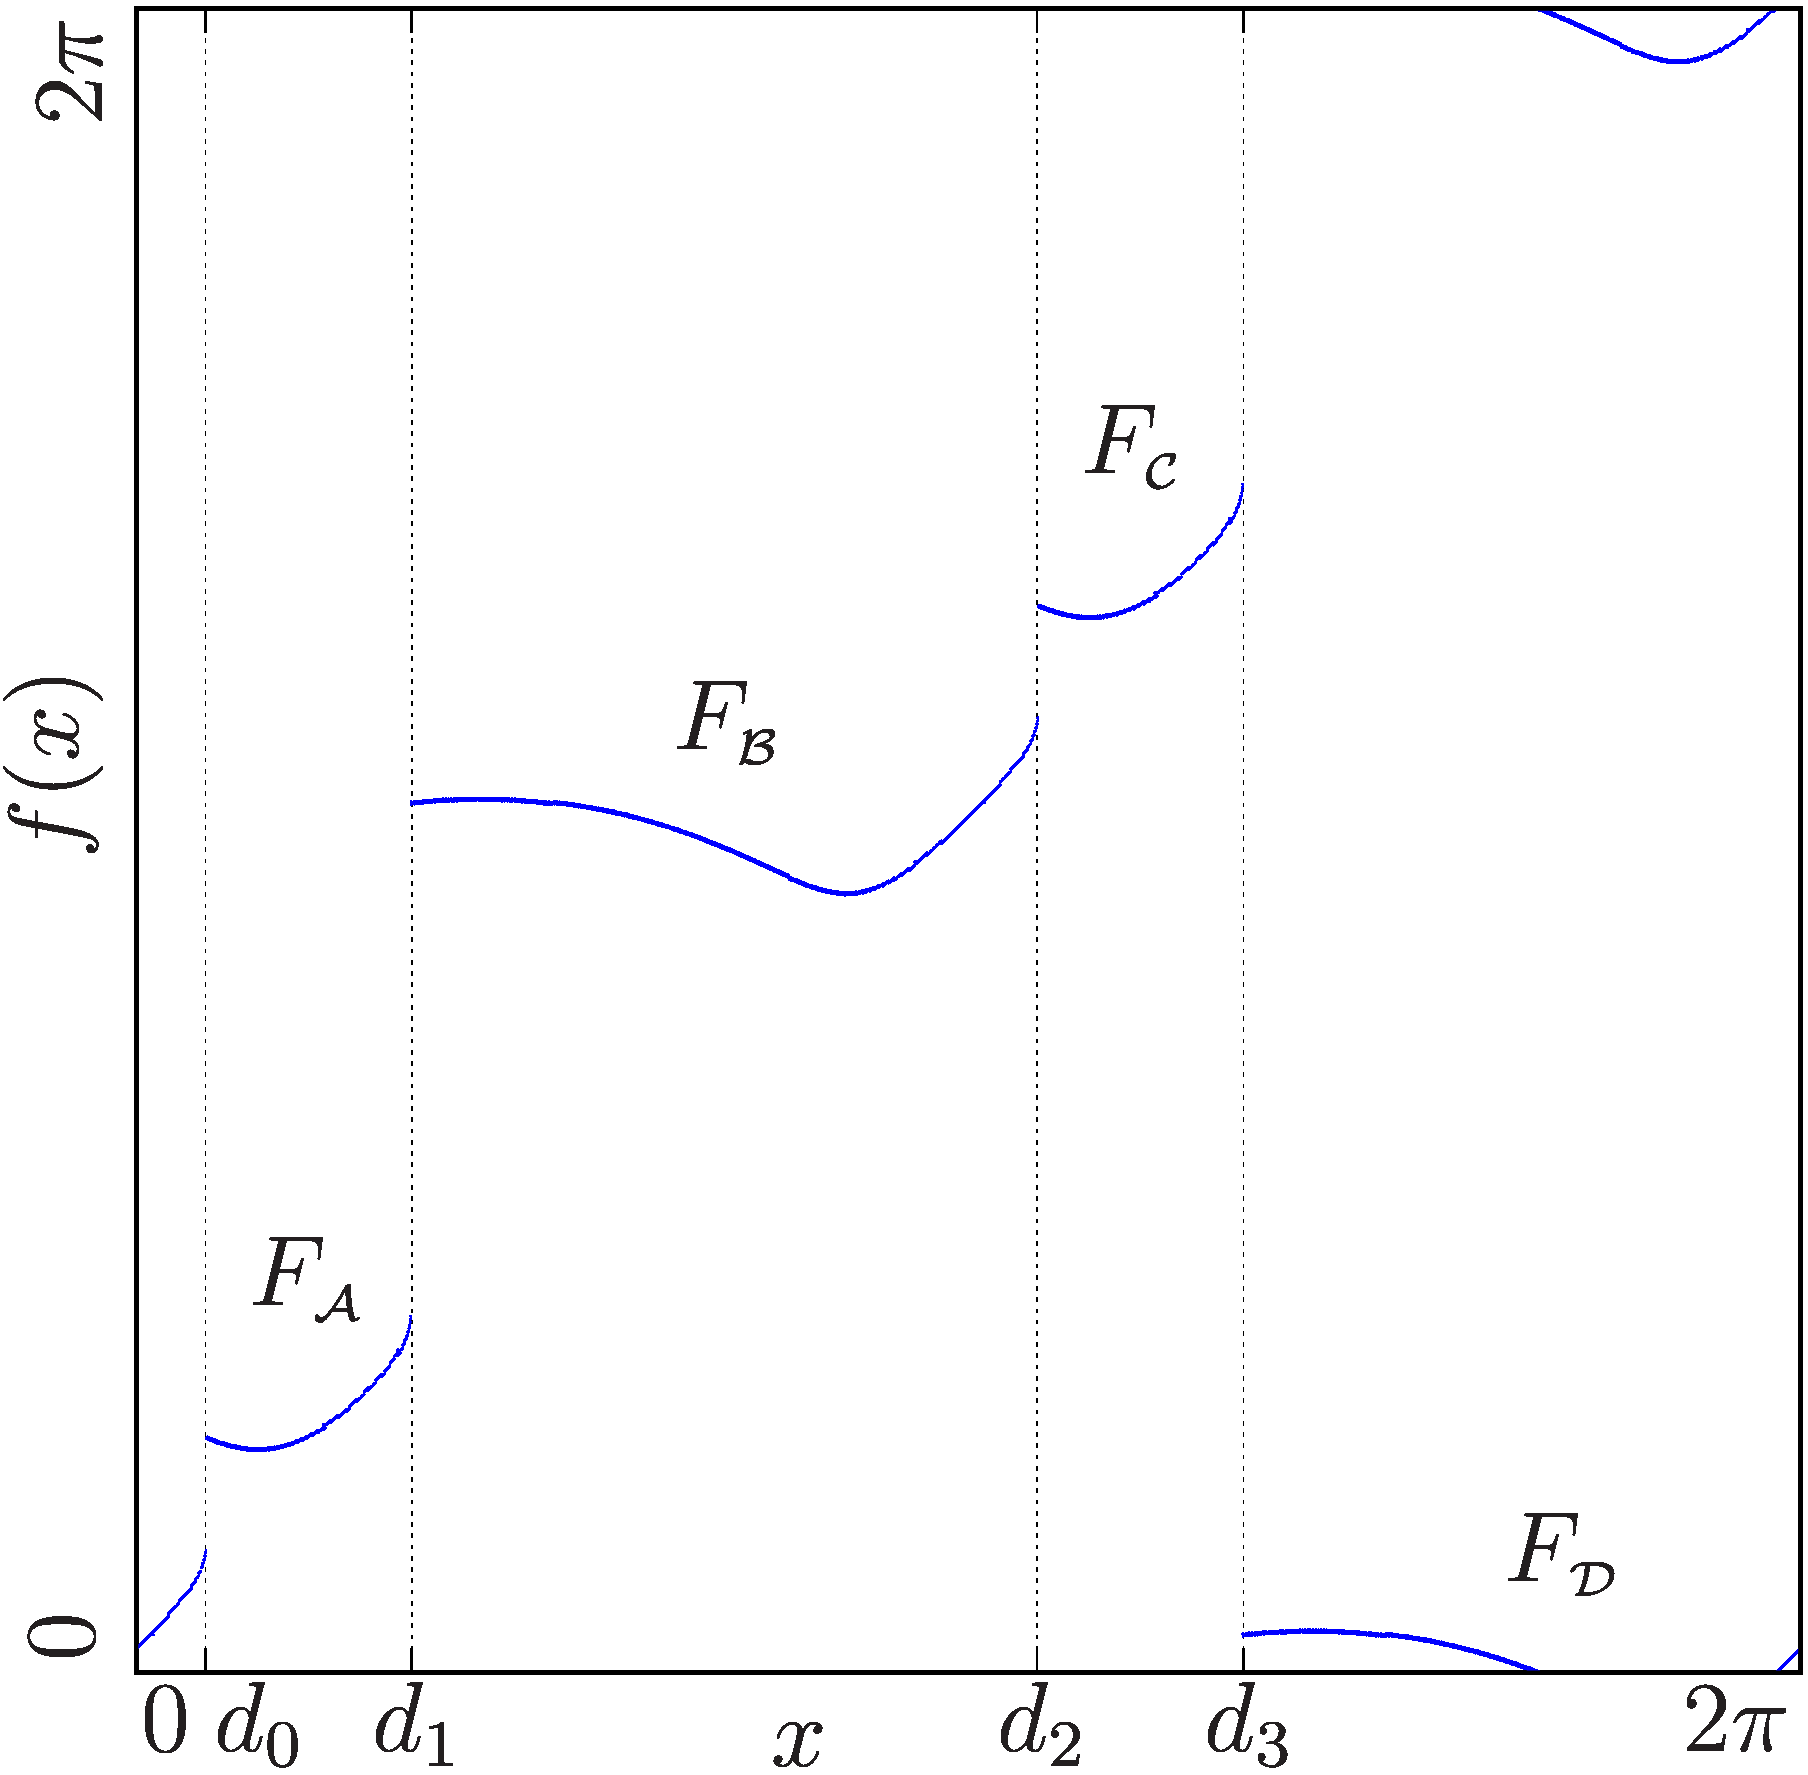
\includegraphics[width=.5 \textwidth]{../Figures/5/5.1/illustration.png}
	\caption[Shape of the original model function]{
		The shape of the original model function at the parameter values $E_0 = 15$ and $\chi_0 = 0.2$.
	}
	\label{fig:setup.char.shape}
\end{figure}

This section is concerned with the overall shape and number of branches of the original model function.

\Cref{fig:setup.char.shape} shows the shape of the original model function.
One can immediately see that the model function has 4 branches.
This is also evident from the model definition given in \Cref{sec:state.og.def}.
Also, we know from \Cref{sec:state.og.dynamics} that the model has the symmetry described by \Cref{equ:state.og.sym}.
So the branches $F_\A$ and $F_\C$ are identical.
The same is true for the branches $F_\B$ and $F_\D$.

There are no fixed points in the parameter regions that this thesis is concerned with.
That means, the function is always larger than the bisector $y=x$.
Also, for the most part the slope of the function is not steep.
Meaning that the absolute value of the model functions derivative is below $1$ for a majority of the state space.
A model where the absolute value of the derivative of its model function is below $1$ for the whole state space is called contractive.
In such a model, every fixed point and cycle is stable.

\subsection{Parameter Effects}
\label{sec:setup.char.paramfx}

This section is concerned with the other types of characteristics, the effects of the parameters of the model on the shape of the model function.
First, it analyzes the combined parameter effects along a chain of parameter regions assocoated with cycles the same period.
After that, it analyzes the isolated effects of the single parameters and decomposes the combined effects into the isolated effects.

\subsection{Combined Effects of Parameters}
\label{sec:setup.char.paramfx.combined}

To replicate the dynamics seen in the model, it is helpful to know, how the model changes along the chains of parameter regions that are associated with cycles of the same period.
This section therefore analyzes the model function at different points in different chains.
\Cref{fig:setup.char.evolution.map} indicates the points used for this analysis.
\Cref{fig:setup.char.evolution.12} shows, how the model function changes along the chain of parameter regions associated with cycles of period 12.
In the figure, there are three functions $F^{A_12}, F^{B_12},$ and $F^{C_12}$.
The function $F^{A_{12}}$ is the model function with the parameters $E_0 = 15.9, \chi_0 = 0.11$.
These parameter values are marked with the point $A_{12}$ in \Cref{fig:setup.char.evolution.map}.
The function $F^{B_{12}}$ is the model function with the parameters $E_0 = 17.07, \chi_0 = 0.182$.
And the function $F^{C_{12}}$ is the model function with the parameters $E_0 = 18.5, \chi_0 = 0.27$.
The parameter values are marked accordingly in \Cref{fig:setup.char.evolution.map}.

\begin{figure}
	\centering
	\subfloat[Points]{
		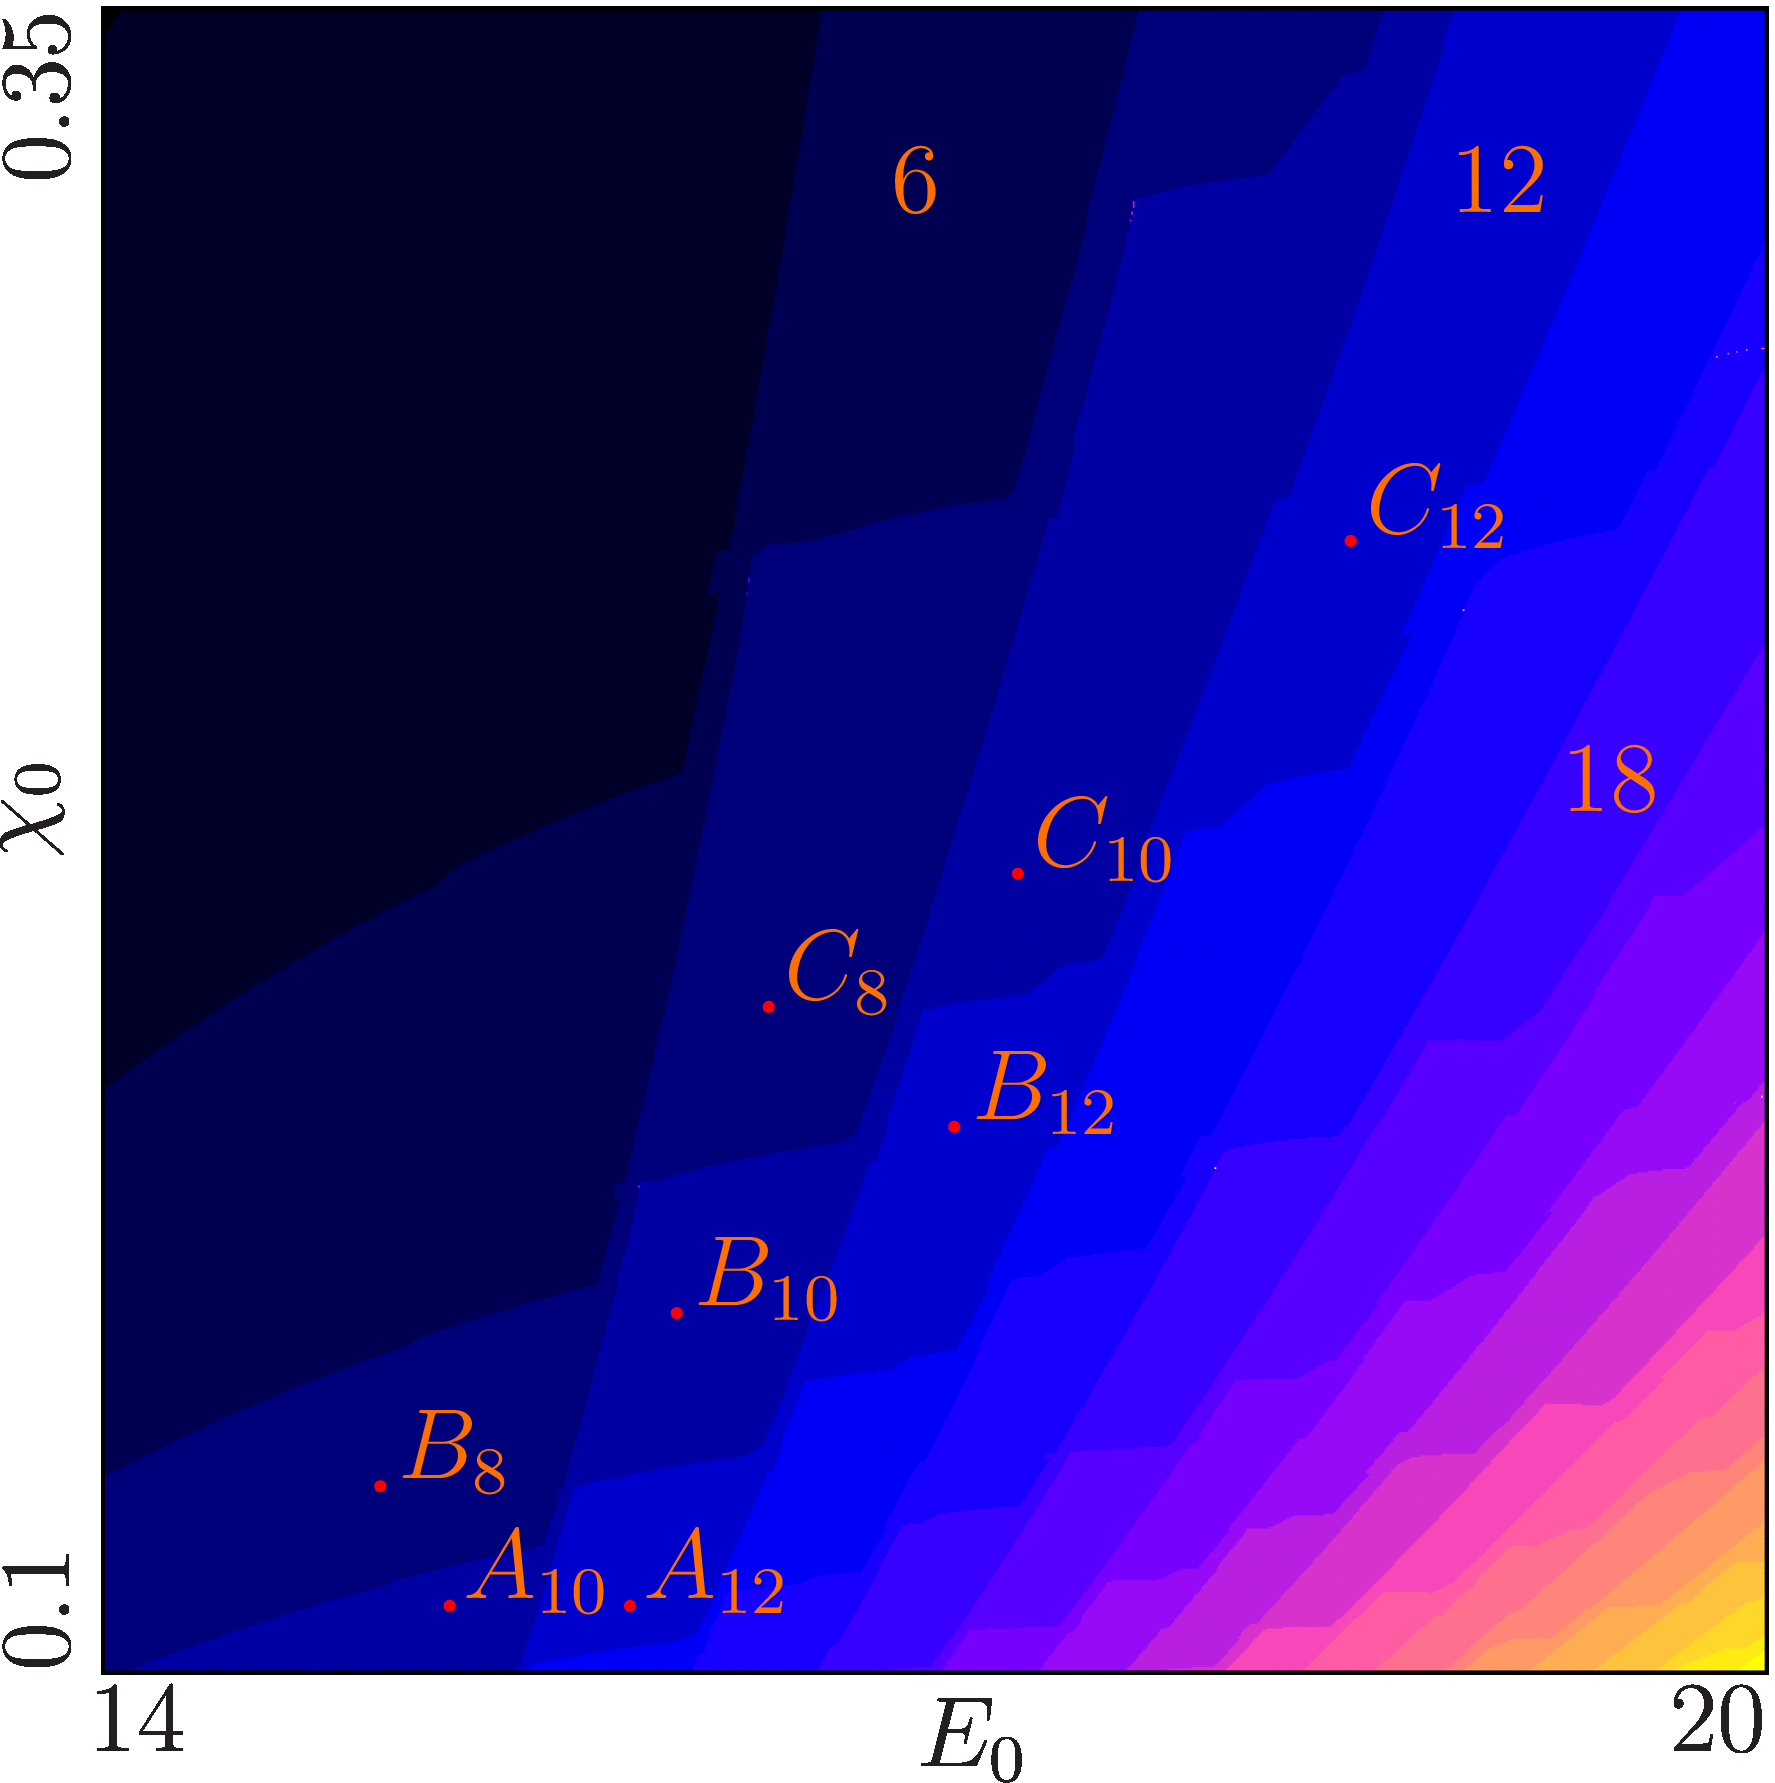
\includegraphics[width=.4 \textwidth]{../Figures/5/5.2a/result.png}
		\label{fig:setup.char.evolution.map}
	}
	\subfloat[Period $12$]{
		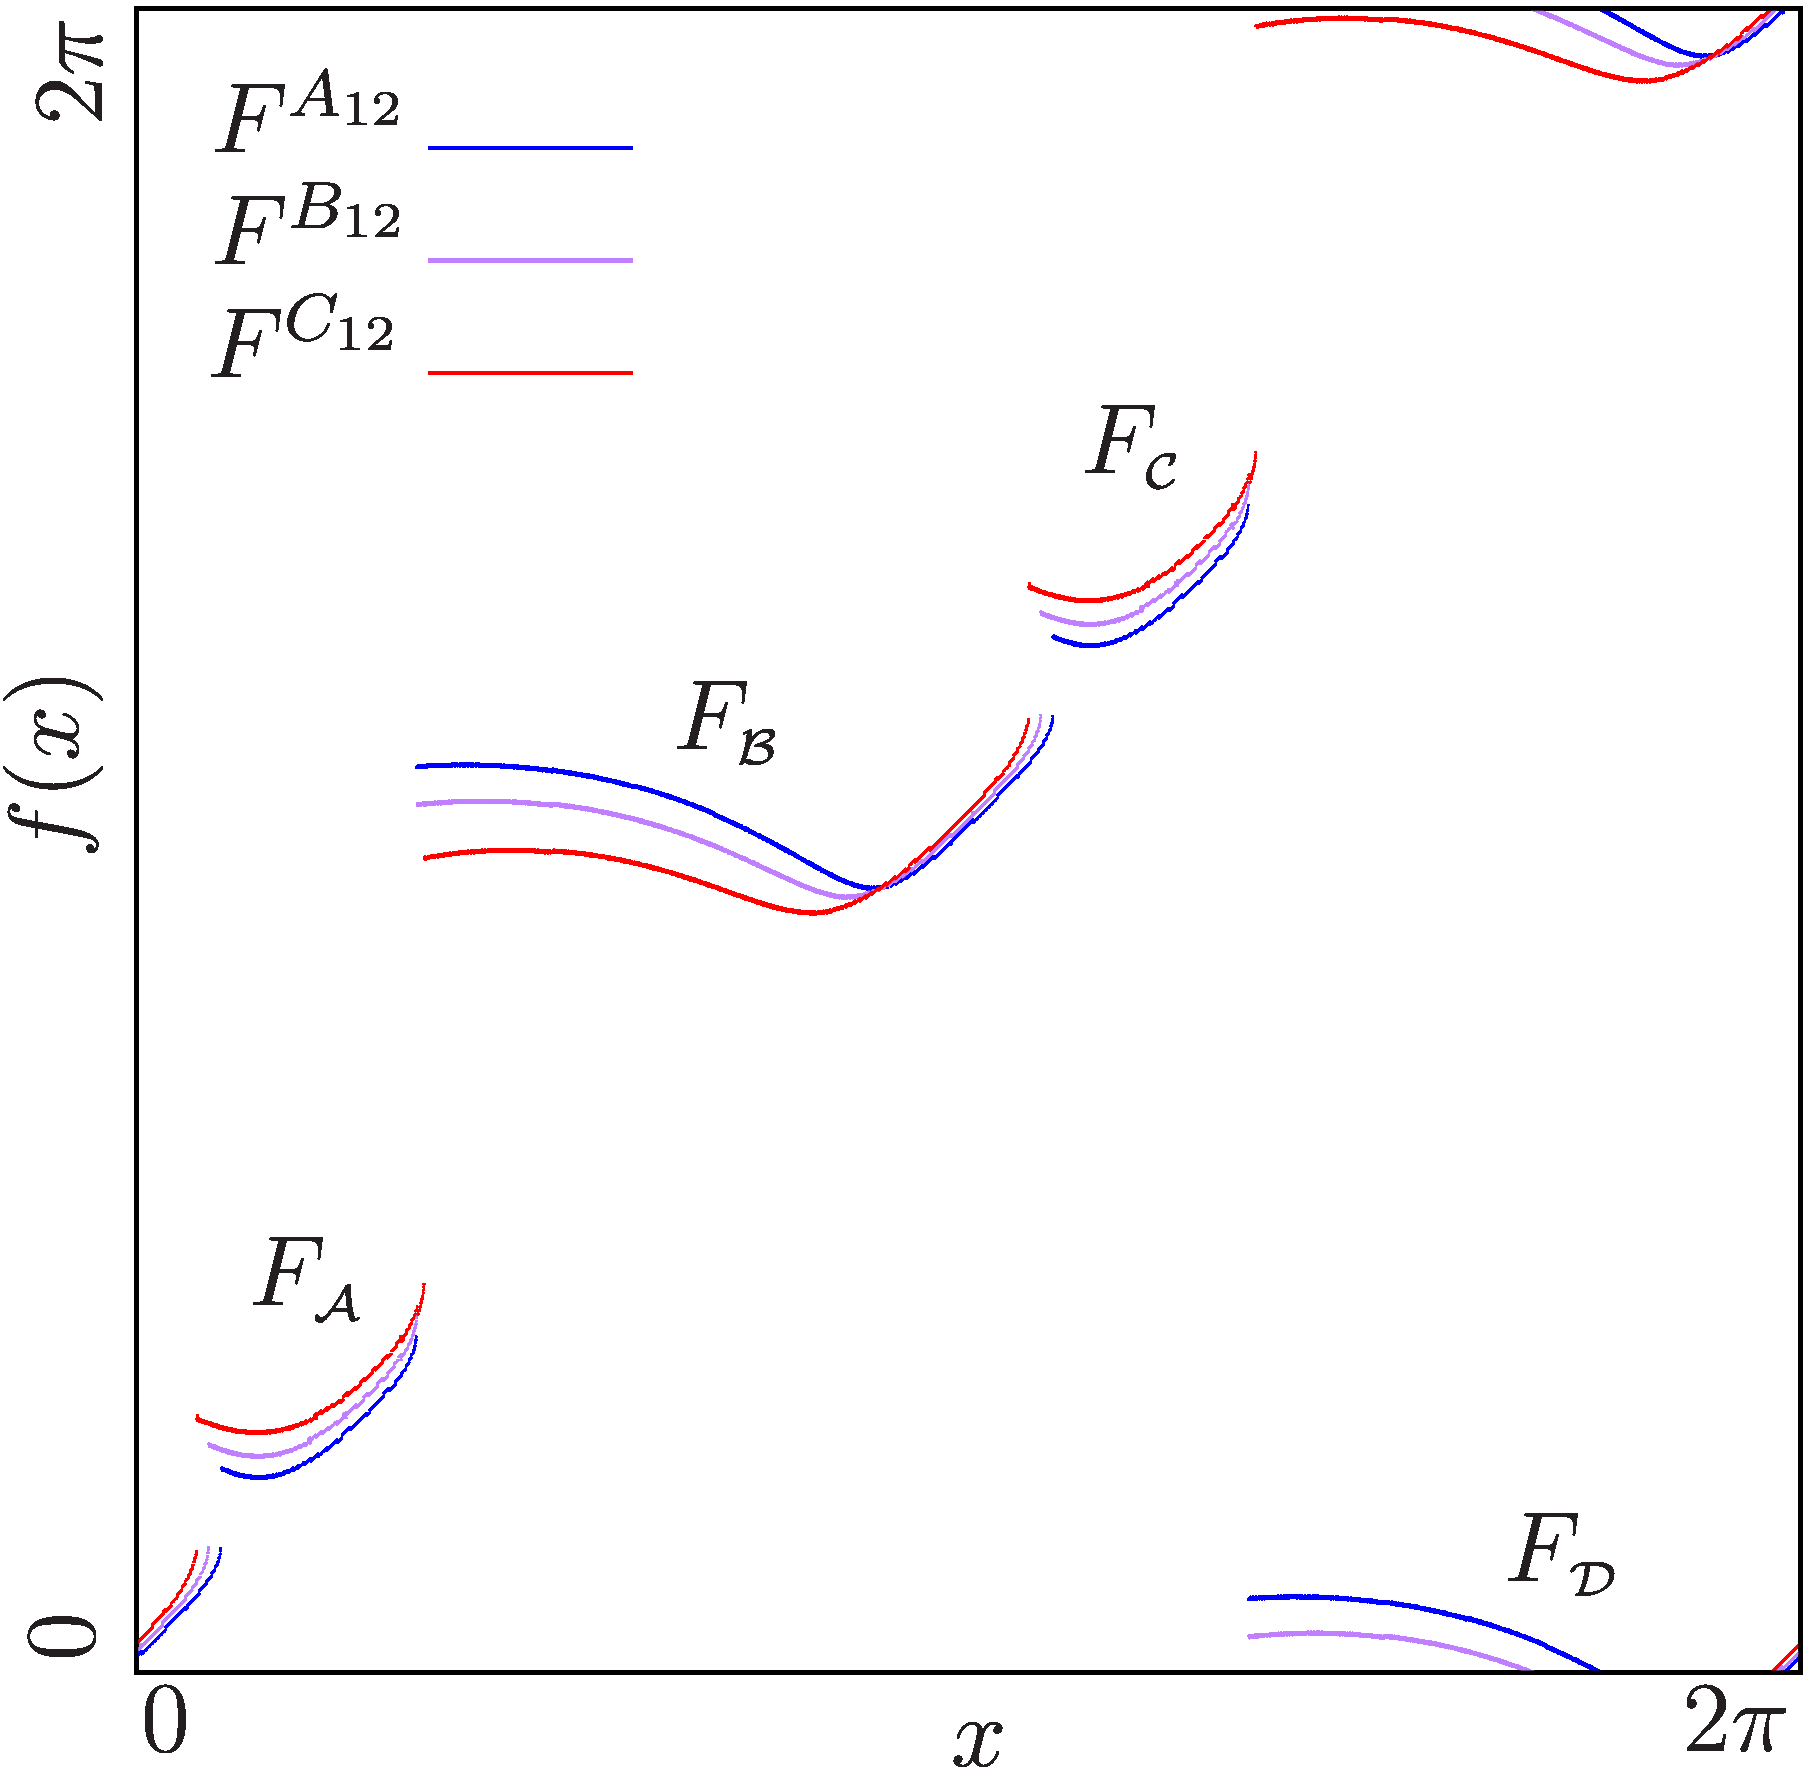
\includegraphics[width=.4 \textwidth]{../Figures/5/5.2b/illustration.png}
		\label{fig:setup.char.evolution.12}
	} \\
	\subfloat[Period $10$]{
		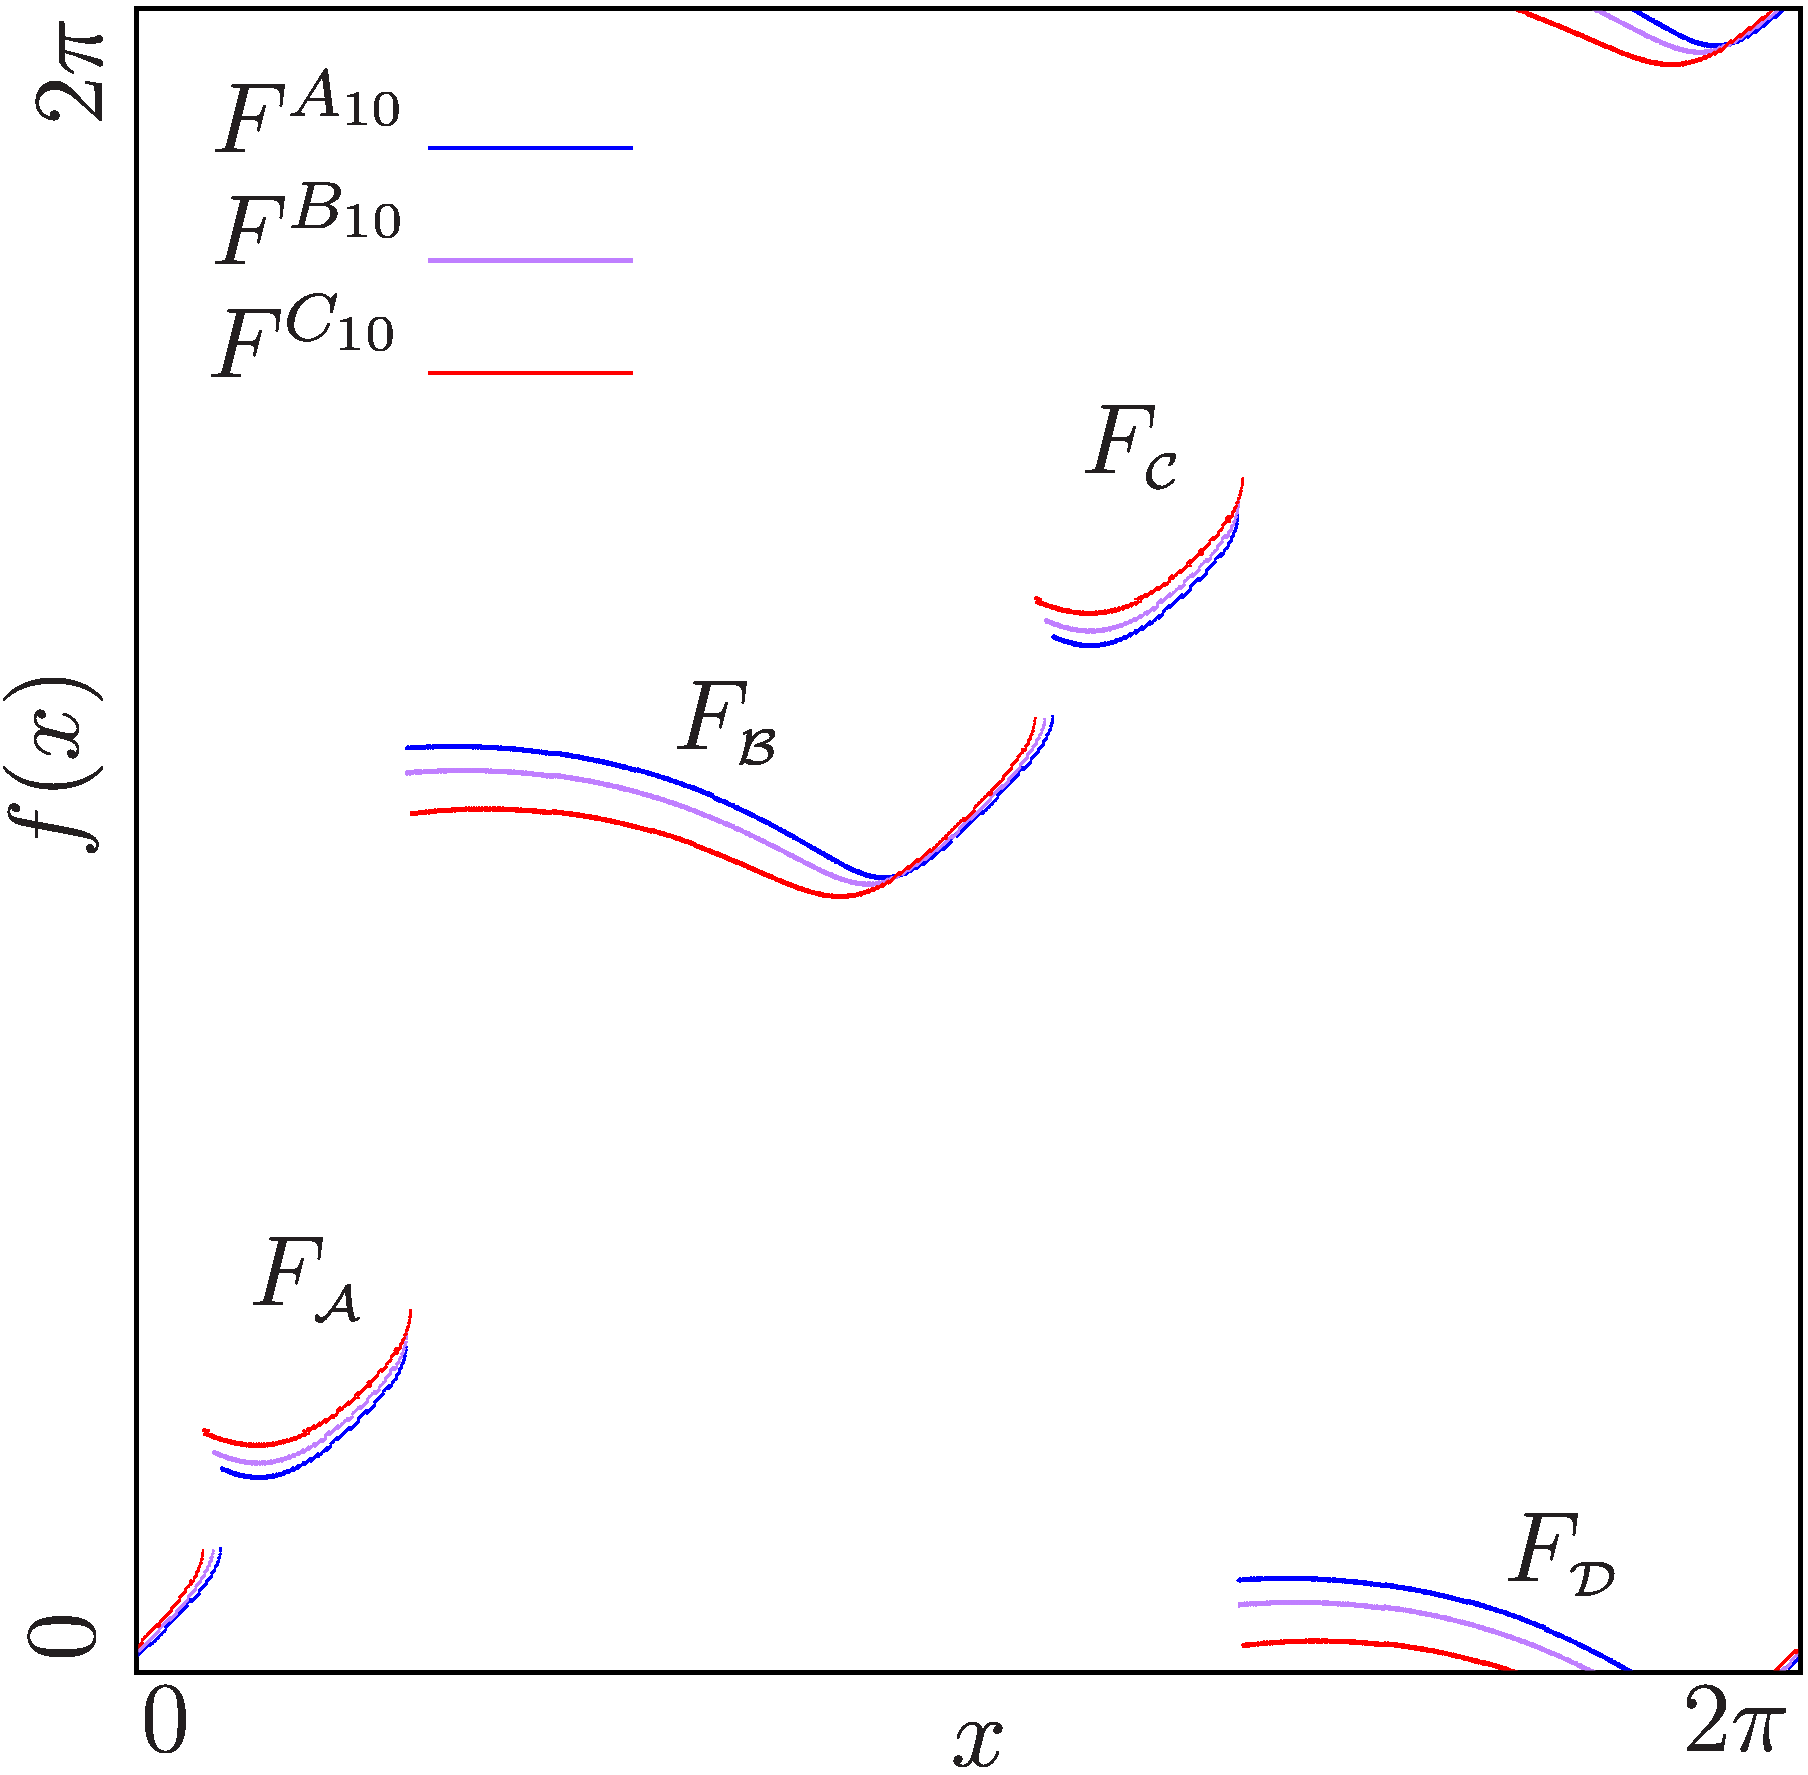
\includegraphics[width=.4 \textwidth]{../Figures/5/5.2c/illustration.png}
		\label{fig:setup.char.evolution.10}
	}
	\subfloat[Period $8$]{
		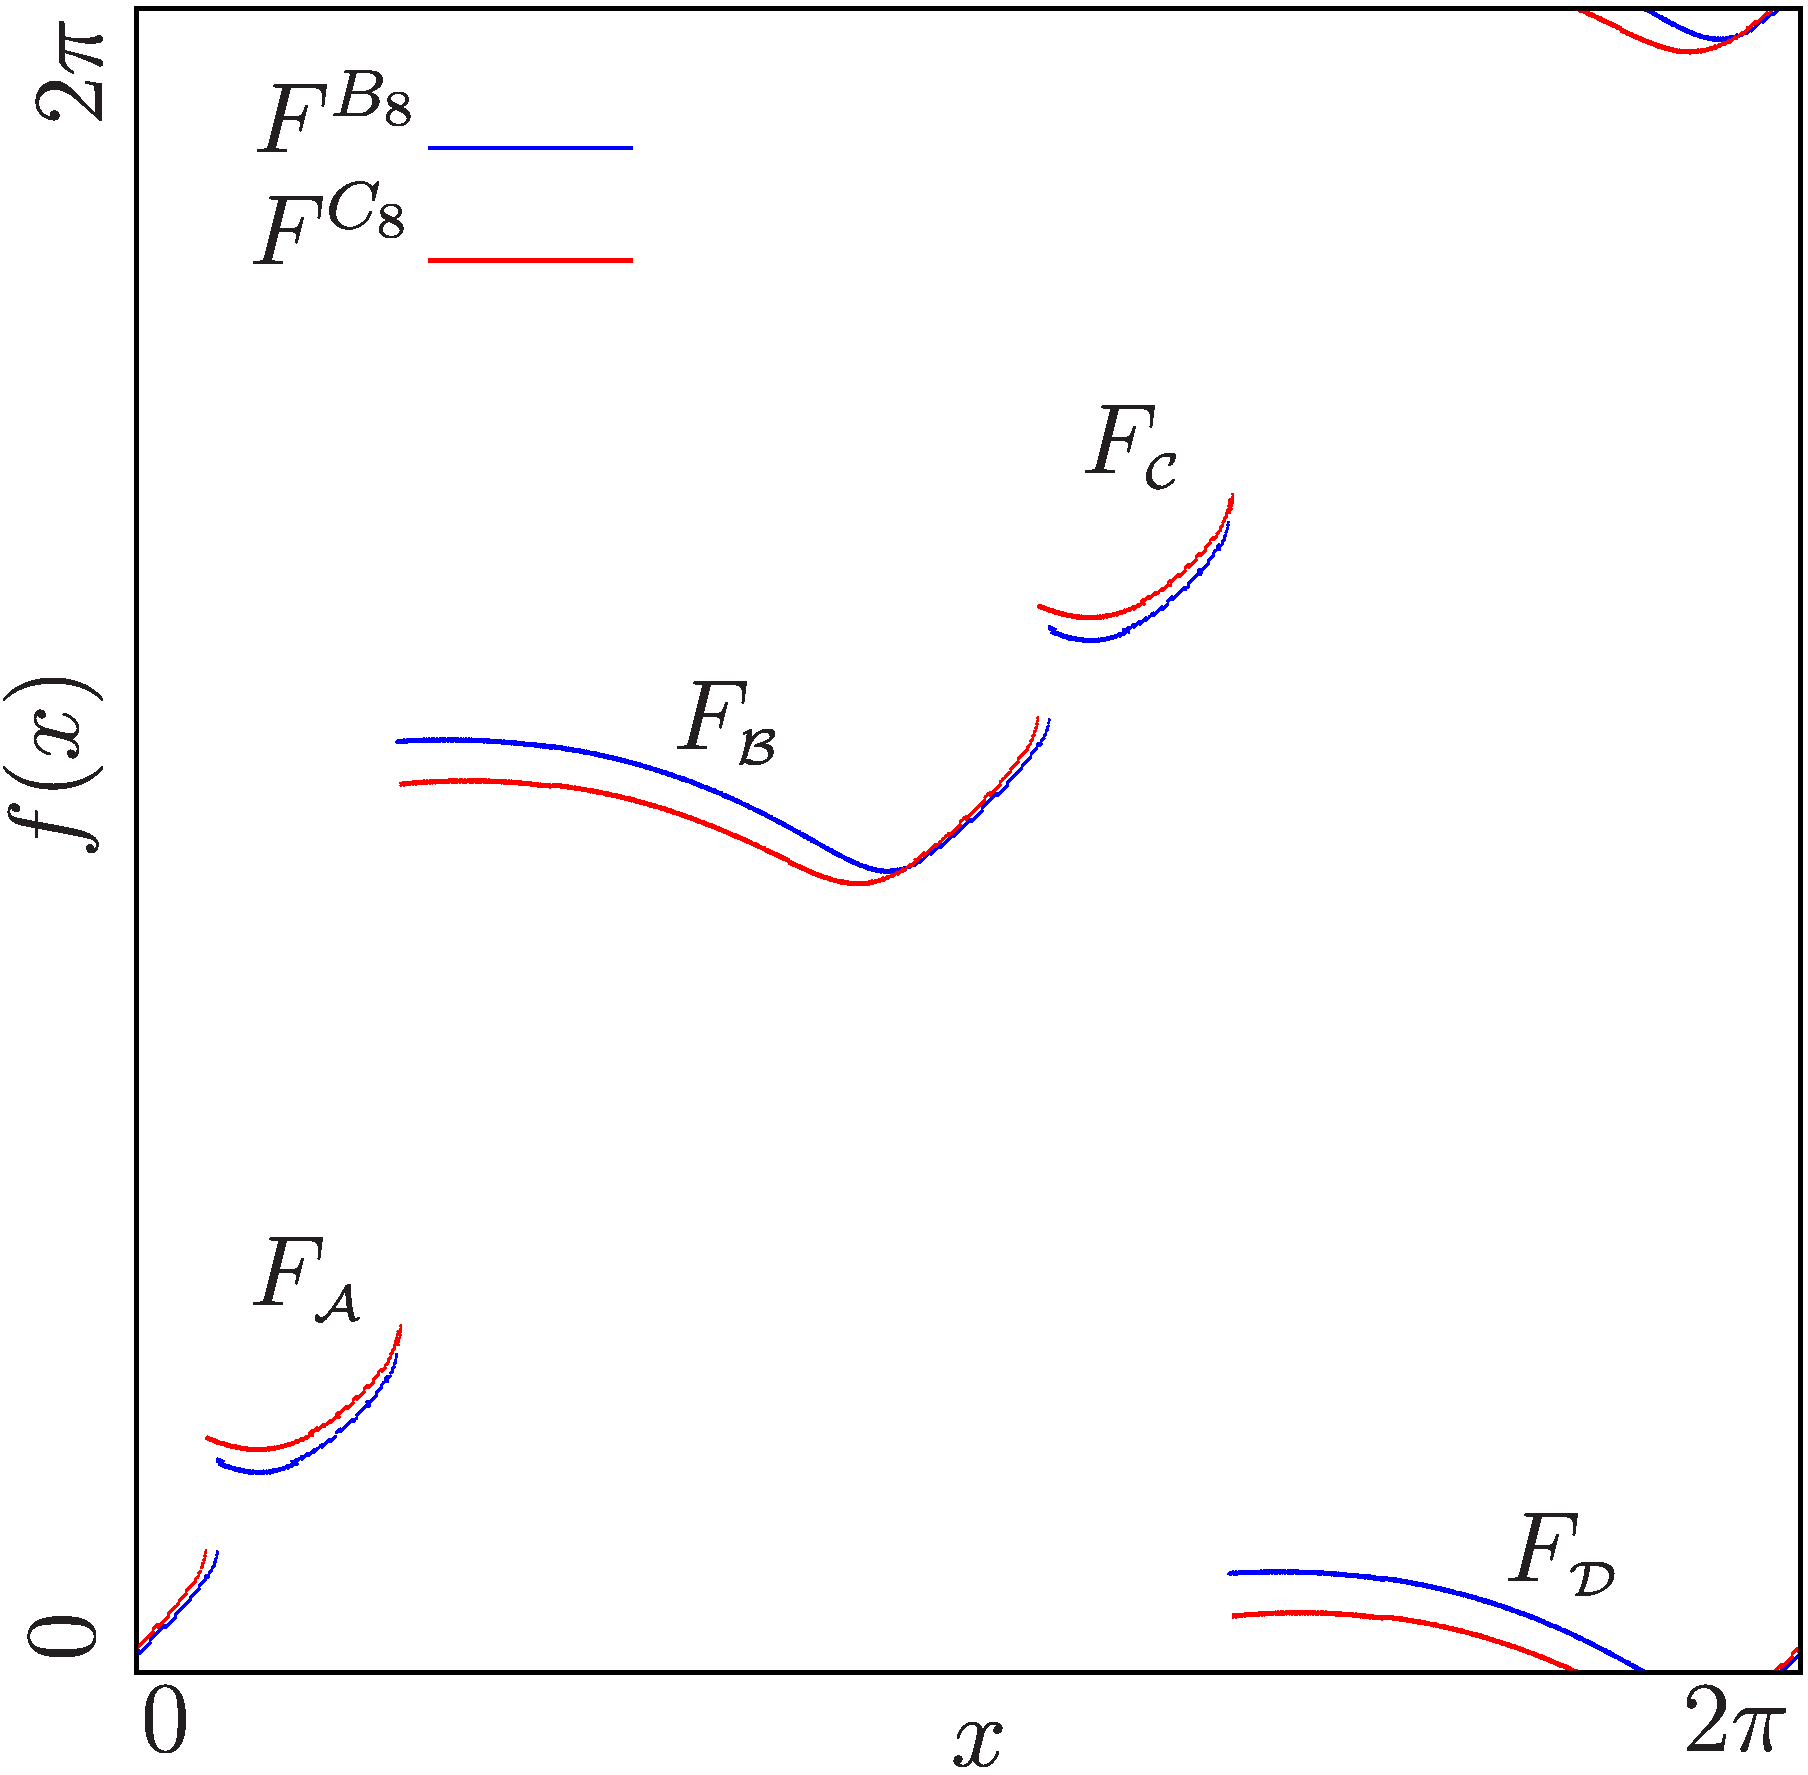
\includegraphics[width=.4 \textwidth]{../Figures/5/5.2d/illustration.png}
		\label{fig:setup.char.evolution.08}
	}
	\caption[The effects of the parameters on the original model function]{
		The effects of the parameters on the original model function illustrated by plotting the model function at different parameter values.
		The parameters $\beta = 1, f = 150, L = 4.2 \cdot 10^{-3}, R = 2, V_m = 5,$ and $\mu = 0.5$ are fixed.
		(a) shows a 2D scan of the periods associated with parameter regions in the original model.
		The parameters $E_0$ and $\chi_0$ are varied in the ranges $[14, 20]$ and $[0.1, 0.35]$.
		The points in this scan mark the parameter values used for plotting the model function in (b), (c), and (d).
		(b) shows the evolution of the shape of the model function along the chain of parameter regions associated with the period 12.
		The function $F^{A_{12}}$ is the model function with the parameter values at the point $A_{12}$ where $E_0 = 15.9$ and $\chi_0 = 0.11$,
		$F^{B_{12}}$ at the point $B_{12}$ where $E_0 = 17.07$ and $\chi_0 = 0.182$,
		and $F^{C_{12}}$ at the point $C_{12}$ where $E_0 = 18.5$ and $\chi_0 = 0.27$.
		(c) shows the evolution of the shape of the model function along the chain of parameter regions associated with the period 10.
		Here, $F^{A_{10}}$ is the model function with the parameters at the point $A_{10}$ where $E_0 = 15.25$ and $\chi_0 = 0.11$,
		$F^{B_{10}}$ at the point $B_{10}$ where $E_0 = 16.07$ and $\chi_0 = 0.154$,
		and $F^{C_{10}}$ at the point $C_{10}$ where $E_0 = 17.3$ and $\chi_0 = 0.22$.
		And (d) shows the evolution of the shape of the model function along the chain of parameter regions associated with the period 8.
		Here, $F^{B_8}$ is the model function with the parameter values at the point $B_8$ where $E_0 = 15$ and $\chi_0 = 0.128$,
		and $F^{C_8}$ at the point $C_8$ where $E_0 = 16.4$ and $\chi_0 = 0.2$.
	}
	\label{fig:setup.char.evolution.combined}
\end{figure}

The most notable changes are the following.
\begin{enumerate}
	\item The values of the whole branches $F_\A$ and $F_\C$ get larger.
	      This change is most notable at the left borders of the branches.
	      The values on the left sides of the branches are affected more by this change than the values on the right sides.
	\item The values on the left sides of the branches $F_\B$ and $F_\D$ get smaller while the values on the right sides are not affected much.
	\item The local minima of the branches $F_\B$ and $F_\D$ move to the left, and their values get smaller.
\end{enumerate}
One smaller change is that the border between branches $F_\B$ and $F_\C$ moves left.
Note that the same change happens to the border between the branches $F_\D$ and $F_\A$ due to the symmetry of the function.

The same effects can be observed in the chains of parameter regions associated with cycles of periods $10$ and $8$, respectively.
For the chain of parameter regions associated with cycles of period $10$, the model function is plotted in \Cref{fig:setup.char.evolution.10} at the three points $A_{10}, B_{10},$ and $C_{10}$ marked in \Cref{fig:setup.char.evolution.map}.
Again, the values of the whole branches $F_\A$ and $F_\C$ are larger in $F^{C_{10}}$ than they are in $F^{A_{10}}$.
And the values on the left sides of the branches $F_\B$ and $F_\D$ are smaller in $F^{C_{10}}$ than they are in $F^{A_{10}}$.
Also, the local minima on those branches move left and down.
For the chain of parameter regions associated with cycles of period $8$, the model function is plotted in \Cref{fig:setup.char.evolution.08} at the two points $B_8$ and $C_8$ marked in \Cref{fig:setup.char.evolution.map}.
And the values of the branches undergo the same changes again from the model function $F^{B_8}$ to $F^{C_8}$.

\subsection{Individual Effects of Parameters}
\label{sec:setup.char.paramfx.individual}

The effects of the parameters described above, always include a change in both parameters $E_0$ and $\chi_0$.
To reproduce the bifurcation structures, it is important to know which effects on the function each parameter has individually.
This section focuses on the isolated effects of each parameter by fixing one of the parameters and only varying the other one and observing the effects of this parameter on the shape of the model function.

\begin{figure}
	\centering
	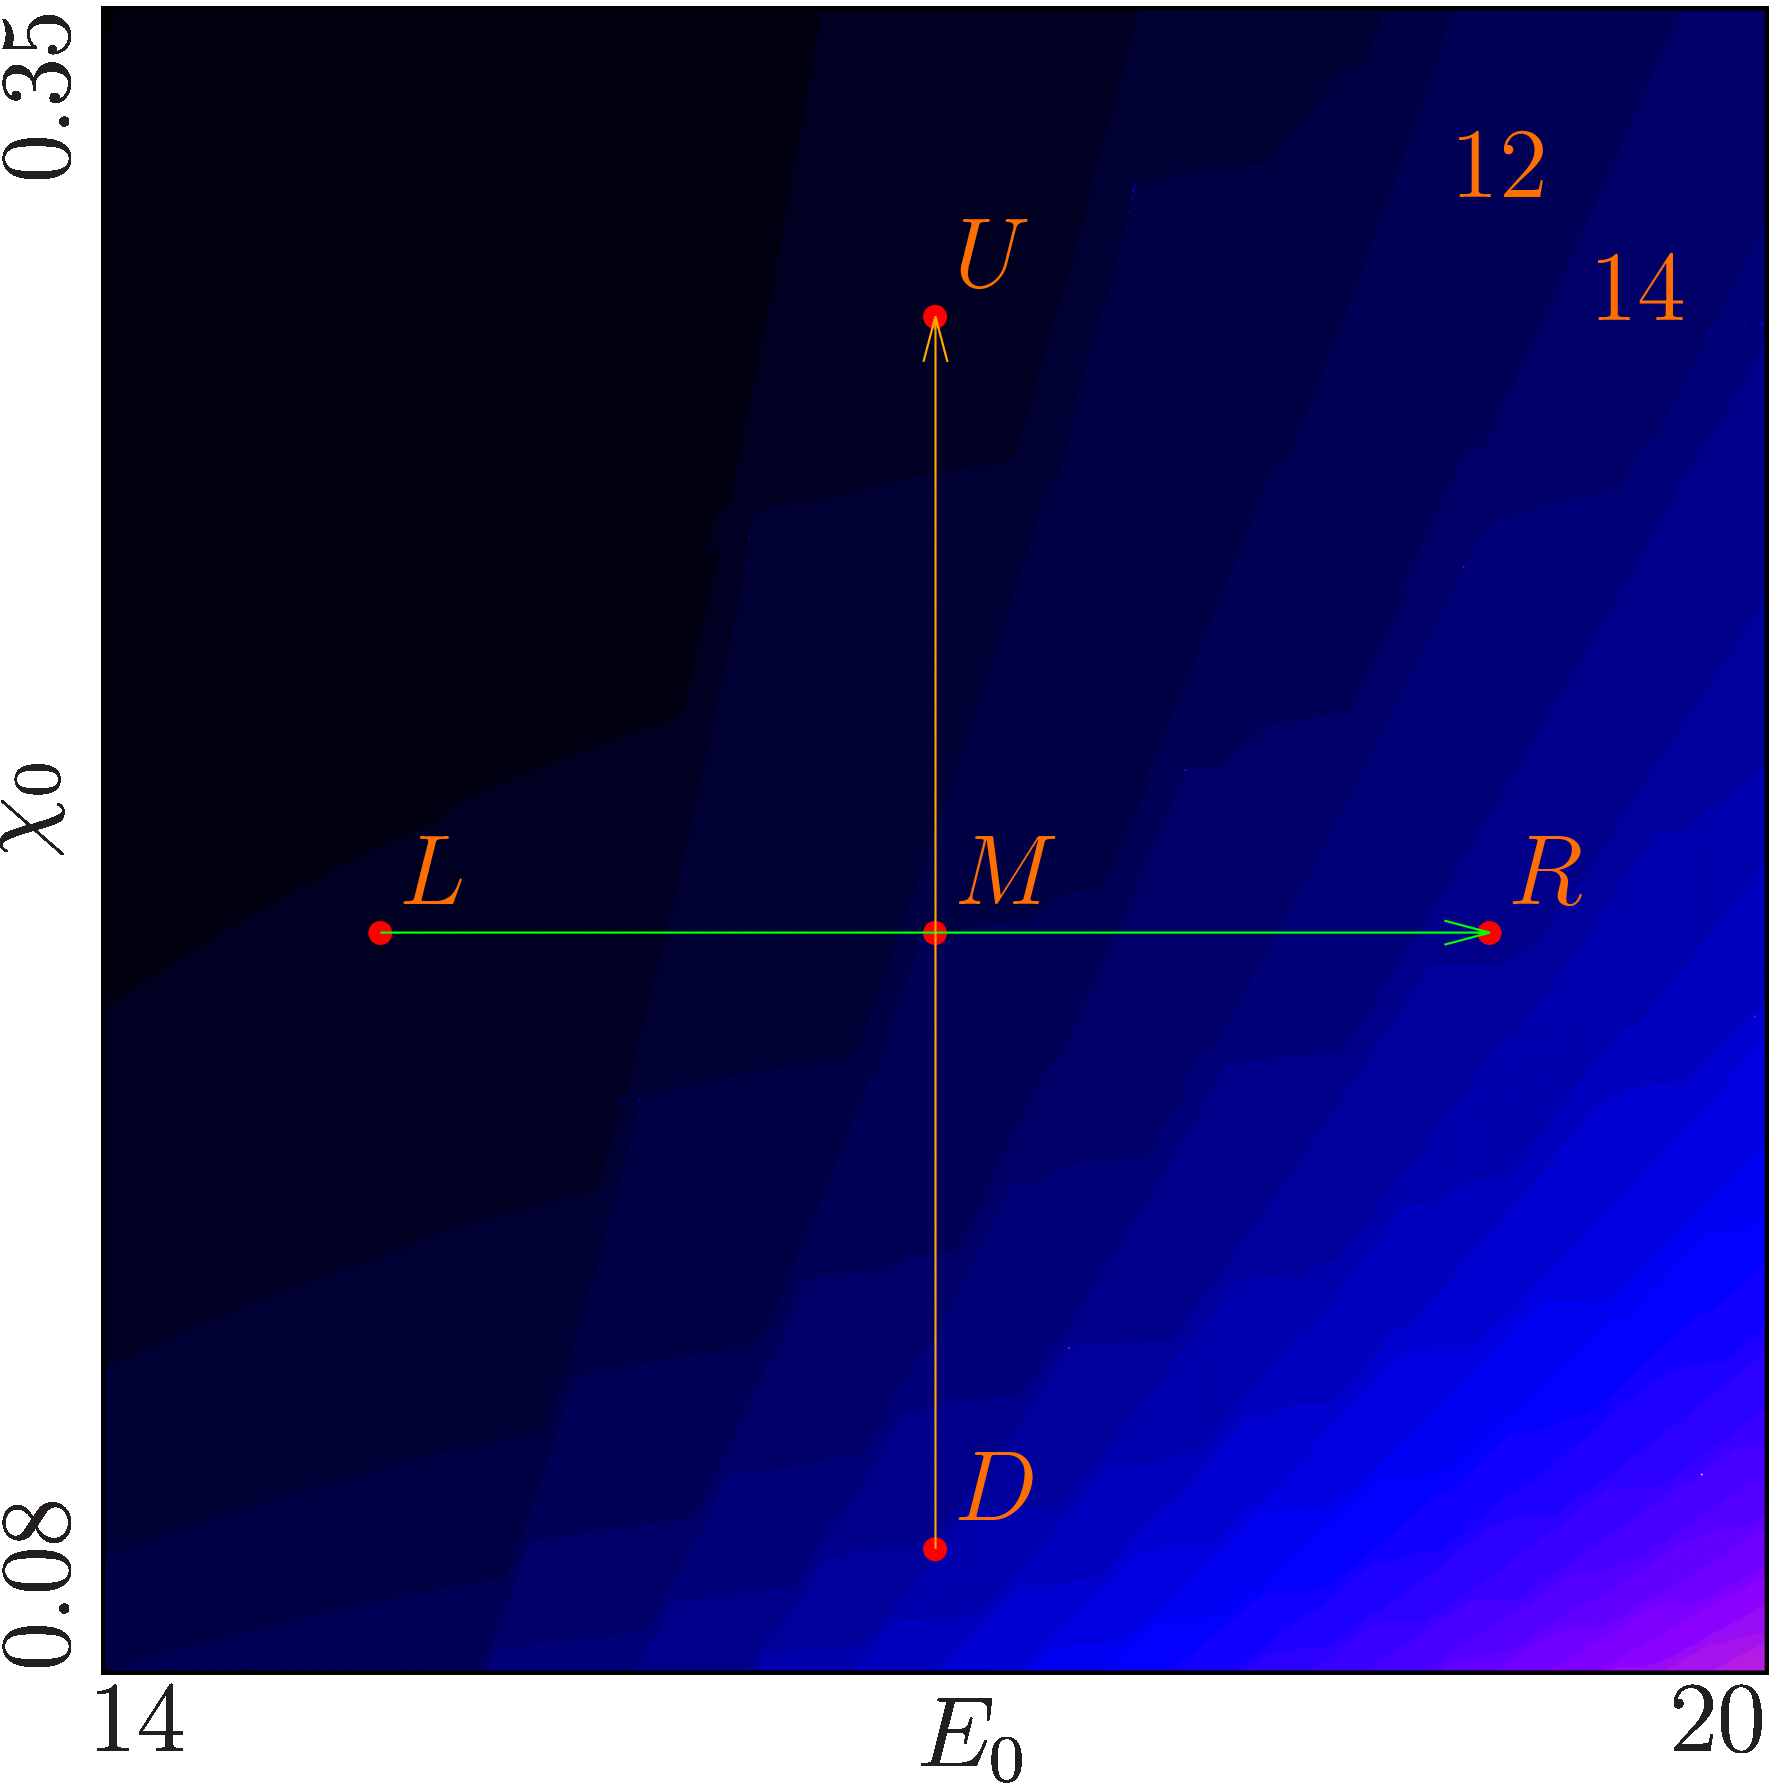
\includegraphics[width=0.4\textwidth]{../Figures/5/5.3/result.png}
	\caption[The parameter ranges examined to analyze the isolated effects of parameters on the original model function]{
		2D scan of the periods associated with parameter regions in the original model.
		The parameters $\beta = 1, f = 150, L = 4.2 \cdot 10^{-3}, R = 2, V_m = 5,$ and $\mu = 0.5$ are fixed.
		The parameters $E_0$ and $\chi_0$ are varied in the ranges $[14, 20]$ and $[0.08, 0.35]$.
		It illustrates the parameter ranges used to analyze the isolated effects of the parameters $E_0$ and $\chi_0$ on the original model function.
		The green arrow indicates the parameter range used to analyze the effects of the parameter $E_0$, while the orange arrow indicates the parameter range used to analyze the effects of the parameter $\chi_0$ on the original model function.
		The points $L, M, R, D,$ and $U$ mark the parameter values used for the cobweb diagrams in \Cref{fig:setup.char.evolution.single}.
	}
	\label{fig:setup.char.evolution.single.map}
\end{figure}

For the effects of the parameter $E_0$, $\chi_0 = 0.2$ is fixed and $E_0$ is varied in the parameter range $[15, 19]$.
This is marked as the green arrow in \Cref{fig:setup.char.evolution.single.map}.
As before, the model function is plotted at three parameter values in one figure.
The functions are visualized in \Cref{fig:setup.char.evolution.e0}.
$F^L$ is the model function with $E_0 = 15$, $F^M$ is the model function with $E_0 = 17$, and $F^R$ is the model function with $E_0 = 17$.
$\chi_0 = 0.2$ is the same for all functions $F^L, F^M,$ and $F^R$.
The parameter values are marked with the points $L, M,$ and $R$ in \Cref{fig:setup.char.evolution.single.map}.
One can see that they are all on the green arrow mentioned before.
The following changes can be observed.
\begin{enumerate}
	\item The values on the left sides of the branches $F_\B$ and $F_\D$ get smaller while the values on the right sides are not affected much.	\item The local minima of the branches $F_\B$ and $F_\D$ move left, and their values get smaller.
	\item The border between the branches $F_\A$ and $F_\B$ moves to the right.
	      The same is true for the border between the branches $F_\C$ and $F_\D$ because of the symmetry in the original model.
	\item The values at the right borders of branches $F_\A$ and $F_\C$ get larger. This is caused by the border between branches $F_\A$ and $F_B$ moving to the right.
\end{enumerate}

For the effects of the parameter $\chi_0$, $E_0 = 17$ is fixed and $\chi_0$ is varied in the parameter range $[0.125, 0.3]$.
This parameter range is marked with an orange arrow in \Cref{fig:setup.char.evolution.single.map}.
Again, the model function is plotted at three parameter values in one figure.
The functions are visualized in \Cref{fig:setup.char.evolution.hi}.
$F^D$ is the model function with $\chi_0 = 0.1$, $F^M$ is the model function with $\chi_0 = 0.2$, and $F^U$ is the model function with $\chi_0 = 0.3$.
$E_0 = 15$ is the same for all functions $F^D, F^M,$ and $F^U$.
The parameter values are marked with the points $D, M,$ and $U$ in \Cref{fig:setup.char.evolution.single.map}.
One can see that they are all on the orange arrow mentioned before.
The following pronounced changes can be observed.
\begin{enumerate}
	\item The values of the whole branches $F_\A$ and $F_\C$ get larger.
	\item The border between the branches $F_\A$ and $F_\B$ moves to the left.
	      The same is true for the border between the branches $F_\C$ and $F_\D$.
\end{enumerate}
Two other smaller changes that can be observed are the following.
\begin{enumerate}
	\item The values on the right sides of the branches $F_\B$ and $F_\D$ get larger.
	      This includes the values of the local minima on these branches.
	\item The border between the branches $F_\B$ and $F_\C$ moves to the left.
	      The same is true for the border between the branches $F_\D$ and $F_\A$.
\end{enumerate}

\begin{figure}
	\centering
	\subfloat[$E_0$]{
		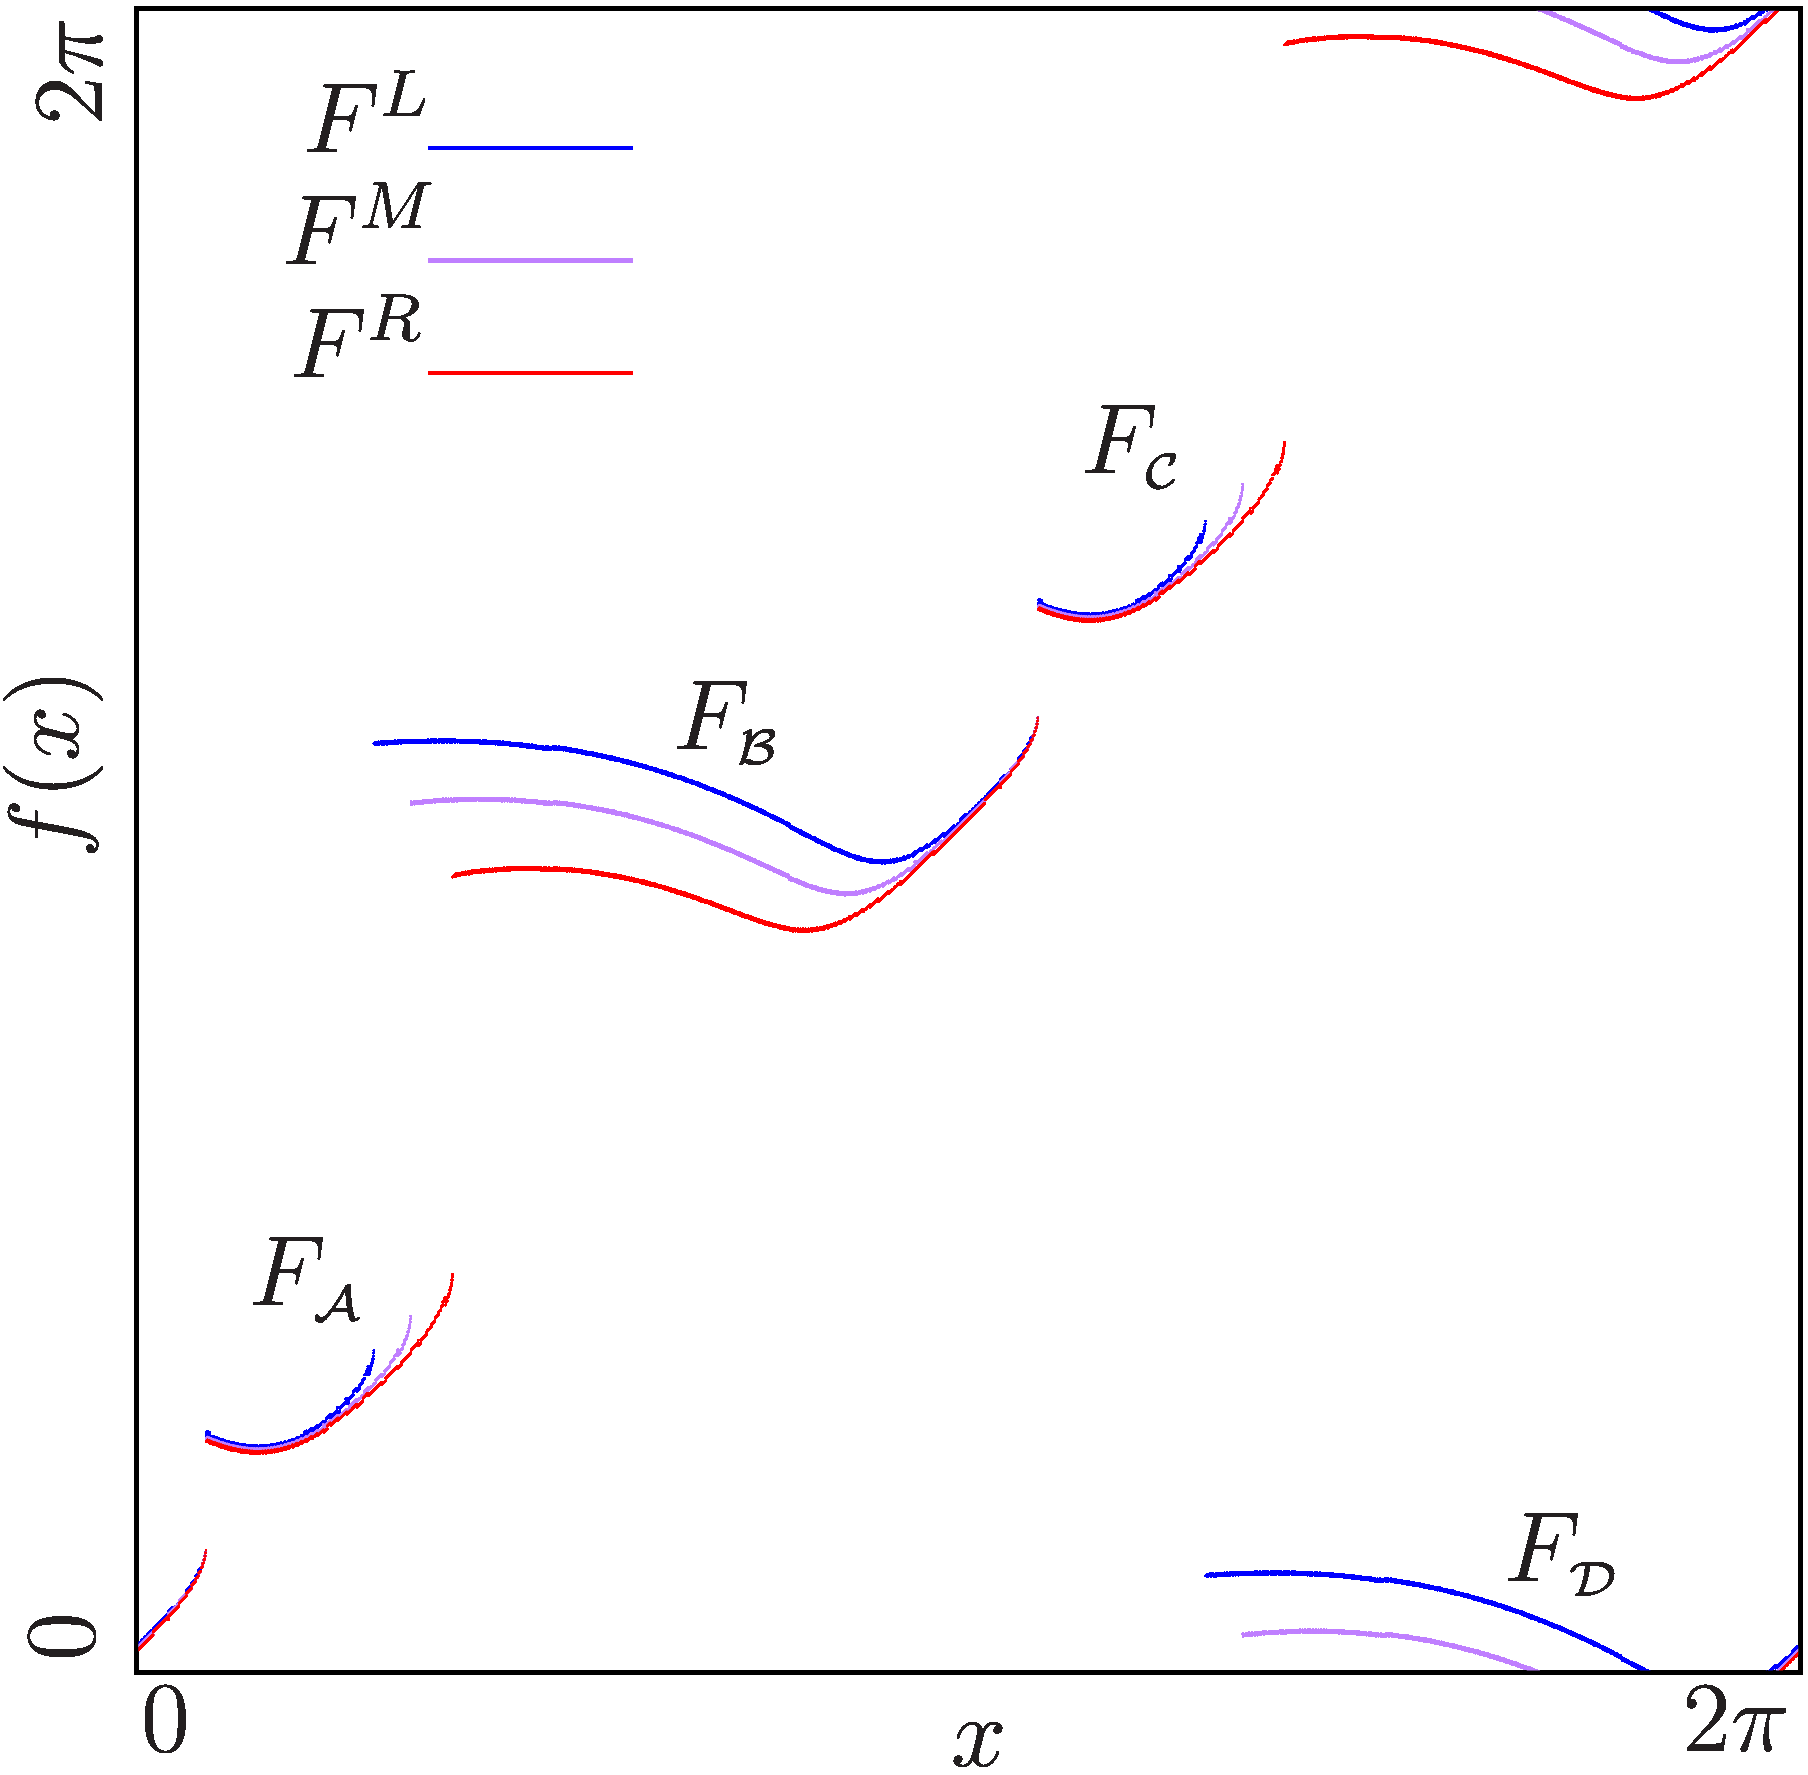
\includegraphics[width=.4 \textwidth]{../Figures/5/5.4a/illustration.png}
		\label{fig:setup.char.evolution.e0}
	}
	\subfloat[$\chi_0$]{
		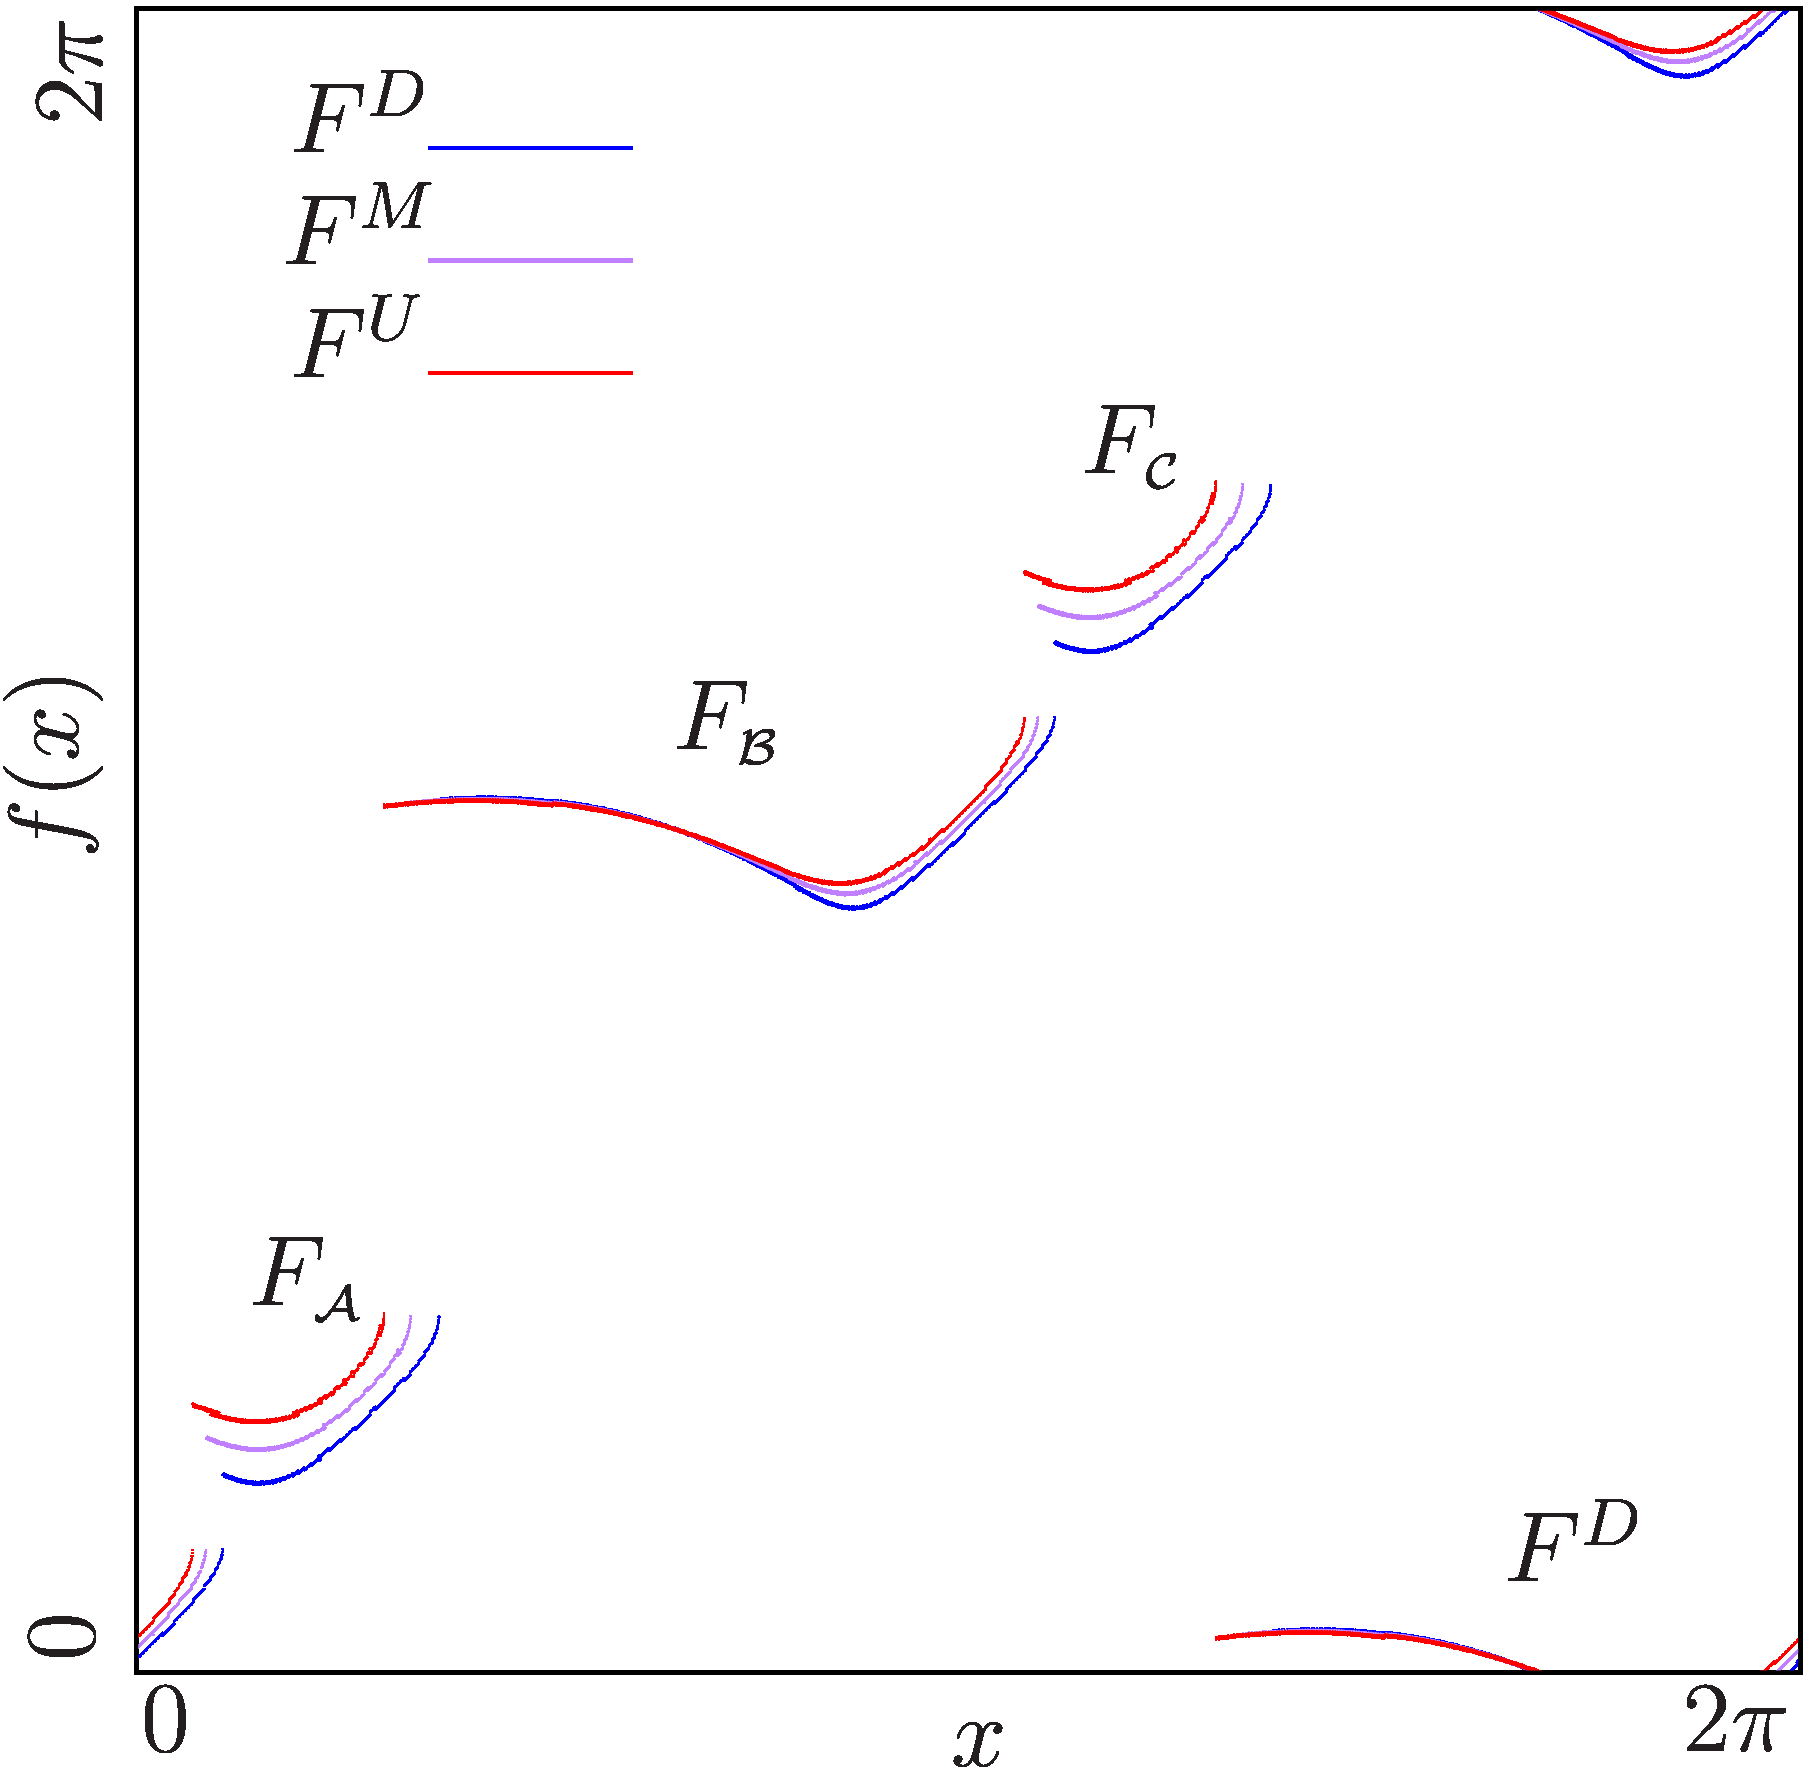
\includegraphics[width=.4 \textwidth]{../Figures/5/5.4b/illustration.png}
		\label{fig:setup.char.evolution.hi}
	}
	\caption[The isolated effects of the parameters on the original model function]{
		The isolated effects of the parameters $E_0$ and $\chi_0$ on the original model function.
		The parameter values used for plotting the functions are marked with points in \Cref{fig:setup.char.evolution.single.map}.
		(a) shows the evolution of the shape of the model function for different parameter values of $E_0$ while $\chi_0 = 0.2$ is fixed.
		The function $F^L$ is the model function with the parameter values at the point $L$ where $E_0 = 15$,
		$F^M$ is at the point $M$ where $E_0 = 17$,
		and $F^R$ is at the point $R$ where $E_0 = 19$.
		(b) shows the evolution of the shape of the model function for different parameter values of $\chi_0$ while $E_0 = 17$ is fixed.
		The function $F^D$ is the model function with the parameter values at the point $D$ where $\chi_0 = 0.1$,
		$F^M$ is at the point $M$ where $\chi_0 = 0.2$,
		and $F^U$ is at the point $U$ where $\chi_0 = 0.3$.
	}
	\label{fig:setup.char.evolution.single}
\end{figure}

\subsection{Decomposition of Combined Effects}
\label{sec:yunus.param.effects.decomposition}

This section considers the decomposition of the combined parameter effects listed in \Cref{sec:setup.char.paramfx.combined} into the effects of the isolated parameter effects listed in \Cref{sec:setup.char.paramfx.individual} and traces each effect back to its cause.
This is important, because some of the isolated parameter effects cancel out when the parameters are both varied as we will see later in this section.
For this, this section introduces a notation for the effects.
The effect of the values on the left side of a branch changing is denoted $\AL$, for the right side it is $\AR$, and for the whole branch it is $\AW$
The subscript indicates, which branch the change affects, and the superscript indicates, whether the values get larger $+$ or smaller $-$.
The effect of changing a local minimum is denoted as $\AMi$.
The meaning of the subscript stays the same as above, but the superscript also can include $L$ for movement to the left and $R$ for movement to the right.
Finally, the effect of moving borders is denoted as $\AB$.
The subscript now includes the two symbols of branches to which the border belongs and the superscript now has only $L$ or $R$.
For brevity, one does not write redundant branch names, so changes happening to branch $F_\A$ are also happening to branch $F_\C$.
For borders, changes to the border between branches $F_\A$ and $F_\B$ are also happening to the border between branches $F_\C$ and $F_\D$ and so on.

\Cref{table:setup.char.paramfx} lists all observed effects along the chains of parameter regions associated with cycles of the same period and their decomposition into effects of the single parameters.
The first part of the table includes all major changes observed in \Cref{sec:setup.char.paramfx.combined}.
The second part includes the minor change one can observe of the borders between the branches $f_\B$ and $f_\C$ moving to the left.
The second part also includes the changes observed in \Cref{sec:setup.char.paramfx.individual} that cancel out.
From this table we can see that $E_0$ causes the effects on the branches $F_\B$ and $F_\D$, while $\chi_0$ causes the changes to the branches $F_\A$ and $F_\C$, as well as the minor movement of the borders between the branches $F_\B$ and $F_\C$.
Note again that the change to the border of branches $F_\B$ and $F_\C$ also applies for the border between branches $F_\D$ and $F_\A$.

% table in next section for better layout



\section{Piecewise Quadratic Model}

In this section, we will examine the dynamics of a piecewise quadratic model.
Starting with a model with 4 branches and symmetry, like in \Cref{sec:og.full}.
After that, we will reduce the model to just two branches using symmetry.

\subsection{Full Model}

The full model is the map $x \mapsto f(x) \mod 6$.
Where $f$ is given by the following collection of equations.
\begin{align}
    f(x) & = \begin{cases}
        g(x) & \text{if } r(x) < 3 \\
        g(x) + 3 & \text{else}
    \end{cases} \label{equ:quad.full.f} \\
    g(x) & = \begin{cases}
        a_L \cdot s_L(x)^2 + b_L \cdot x + c_L & \text{if } s(x) < \frac{3}{2} \\
        a_R \cdot s_R(x)^2 + b_R \cdot x + c_R & \text{else}
    \end{cases} \label{equ:quad.full.g}
\end{align}

\Cref{equ:quad.full.f} causes the disontinuity in the middle at $x = 3$.
It also makes sure, the symmetry $f(x + 3) \equiv f(x) + 3 \mod 6$ is true.
Each half of the model is then governed by \Cref{equ:quad.full.g}.
Here all the 6 parameters $a_L, a_R, b_L, b_R, c_L,$ and $c_R$ act.

\Crefrange{equ:quad.full.s}{equ:quad.full.sr} provide adjusted values of x for either choosing between branches in both halves or substituting in the quadratic formulas of each branch.
\begin{subequations}
\begin{align}
    s(x) & = x \mod 3 \label{equ:quad.full.s} \\
    s_L(x) & = s(x) - \frac{3}{4} \\
    s_R(x) & = s(x) - \frac{9}{4} \label{equ:quad.full.sr}
\end{align}
\end{subequations}

\Cref{fig:quadratic.full.2d.full} shows a 2D-scan of the periods of the stable cycles.
The parameters $a_L = a_R = 1$ and $b_L = b_R = 0$ are fixed and the parameters $c_L$ and $c_R$ are varied.
Both are varied within the range $[0, 6]$ because beyond that the diagram just repeats infinitely.
The structure in the middle left is enhanced and depicted in \Cref{fig:quadratic.full.2d.z1}.

\begin{figure}
    \centering
    \begin{subfigure}{0.4\textwidth}
        \centering
        \includegraphics[width=\textwidth]{21_Quadratic_mod6/2D_Period_Full/result.png}
        \caption{Full}
        \label{fig:quadratic.full.2d.full}
    \end{subfigure}
    \begin{subfigure}{0.4\textwidth}
        \centering
        \includegraphics[width=\textwidth]{21_Quadratic_mod6/2D_Period_Zoomed1/result.png}
        \caption{Zoomed}
        \label{fig:quadratic.full.2d.z1}
    \end{subfigure}
    \caption{2D Scan of Full Quadratic Model}
\end{figure}

A phenomenon like in the original model could not be found here.
But something very similar happens on the border of these wings.
\Cref{fig:quad.full.Cobwebs} shows the cobwebs along the line marked in \Cref{fig:quadratic.full.2d.z1}.
Before the border, there is one stable cycle with period 8.
This cycle is depicted in \Cref{fig:quad.full.CobwebA} and its symbolic sequence is $\A^3B\C^3\D$.
At the border, there is an area where two cycles coexist.
You cannot see this in the 2D scans above, since it only ever picks up on one cycle.
\Cref{fig:quad.full.CobwebB} shows the coexisting cycles at this border.
In contrast to the original model, the cycle that existed before in \Cref{fig:quad.full.CobwebA}, still exists alongside the new cycle with period 6.
The symbolic sequence of the new cycle is $\A^2\B\C^2\D$.

This is different from the dynamics in the original model in two ways.
First, the cycles before and after the area of coexistence have different periods.
And second, the cycles existing outside the area of coexistence still exist inside the area of coexistence.
In the original model, the cycles existing outside the area of coexistence would disappear at the border and new cycles would emerge inside this area.

\begin{figure}
    \centering
    \begin{subfigure}{0.3\textwidth}
        \centering
        \includegraphics[width=\textwidth]{21_Quadratic_mod6/Cobweb_A/result.png}
        \caption{Before border}
        \label{fig:quad.full.CobwebA}
    \end{subfigure}
    \begin{subfigure}{0.3\textwidth}
        \centering
        \includegraphics[width=\textwidth]{21_Quadratic_mod6/Cobweb_B/result.png}
        \caption{At border}
        \label{fig:quad.full.CobwebB}
    \end{subfigure}
    \begin{subfigure}{0.3\textwidth}
        \centering
        \includegraphics[width=\textwidth]{21_Quadratic_mod6/Cobweb_C/result.png}
        \caption{After border}
        \label{fig:quad.full.CobwebC}
    \end{subfigure}
    \caption{Cobwebs along marked line}
    \label{fig:quad.full.Cobwebs}
\end{figure}


\section{Piecewise Quadratic Model with Hyperparameters}

Now we will attempt to imitate the effects of the parameter $E_0$ on the branches $f_\B$ and $f_\D$ better.
Previously, we just varied $c_R$ which changes the values of the whole branches evenly.
Now, we only want to affect the value at the left borders of these branches.
For this, we introduce new parameters that are tied directly to characteristics of the model function.

\subsection{Parameter Definitions}

The new parameters are $g_R\left(\frac{1}{4}\right)$ for the value at the left border of branches $f_\B$ and $f_\D$, $g_R\left(\frac{1}{2}\right)$ for the value at the right border of the branches, and finally $\left. \frac{d}{dx} g_R(x) \right|_{x = \frac{1}{2}}$ for the slope of the branches at the right border.
We fix the parameter $\left. \frac{d}{dx} g_R(x) \right|_{x = \frac{1}{2}} = 1.2$.
This way, the steepest slope is 1.2 which is just above 1.
Therefore, most of the function is still contractive.
We also fix the parameter $g_R\left(\frac{1}{2}\right) = \frac{1}{2} + \epsilon$ with $\epsilon = 0.025$ to have the value at the right border of the branches just above the bisector $y = x$.
The parameter left is $g_R\left(\frac{1}{4}\right)$, the value at the left border of the branches.
This parameter is varied.

\begin{subequations}
	\begin{align}
		g_R\left(\frac{1}{4}\right)                                     & = a_R \cdot \left(\frac{1}{4}\right)^2 + b_R \cdot \left(\frac{1}{4}\right) + c_R = \dfrac{a_R}{16} + \dfrac{b_R}{4} + c_R \label{equ:setup.quad.hyper.A} \\
		g_R\left(\frac{1}{2}\right)                                     & = a_R \cdot \left(\frac{1}{2}\right)^2 + b_R \cdot \left(\frac{1}{2}\right) + c_R = \dfrac{a_R}{4} + \dfrac{b_R}{2} + c_R \label{equ:setup.quad.hyper.B}  \\
		\left. \frac{d}{dx} g_R\left(x\right) \right|_{x = \frac{1}{2}} & = 2 \cdot a_R \cdot \left(\frac{1}{2}\right) + b_R \label{equ:setup.quad.hyper.C}
	\end{align}
\end{subequations}

\Crefrange{equ:setup.quad.hyper.A}{equ:setup.quad.hyper.A} are the values of $g_R\left(\frac{1}{4}\right), g_R\left(\frac{1}{2}\right),$ and $\left. \frac{d}{dx} g_R\left(x\right) \right|_{x = \frac{1}{2}}$.
This is a system of equations, we now need to solve for the parameters $a_R, b_R,$ and $c_R$.
To compute the parameters, we write the system as a matrix and invert it.
The matrix and its inverse are in \Cref{equ:setup.quad.hyper.matrix}.

\begin{align}
	\begin{pmatrix}
		\frac{1}{16} & \frac{1}{4} & 1 \\
		\frac{1}{4}  & \frac{1}{2} & 1 \\
		1            & 1           & 0
	\end{pmatrix}^{-1} & =
	\begin{pmatrix}
		16  & -16 & 4           \\
		-16 & 16  & -3          \\
		4   & -3  & \frac{1}{2}
	\end{pmatrix}
	\label{equ:setup.quad.hyper.matrix}
\end{align}

Hence, the equations for $a_R, b_R,$ and $c_R$ in dependence of $g_R\left(\frac{1}{4}\right), g_R\left(\frac{1}{2}\right),$ and $\left. \frac{d}{dx} g_R\left(x\right) \right|_{x = \frac{1}{2}}$ are \Crefrange{equ:setup.quad.hyper.aR}{equ:setup.quad.hyper.cR}.

\begin{align}
	a_R & = 16 \cdot g_R\left(\frac{1}{4}\right) - 16 \cdot g_R\left(\frac{1}{2}\right) + 4 \cdot \left. \frac{d}{dx} g_R\left(x\right) \right|_{x = \frac{1}{2}}     \label{equ:setup.quad.hyper.aR}     \\
	b_R & = -16 \cdot g_R\left(\frac{1}{4}\right) + 16 \cdot g_R\left(\frac{1}{2}\right) - 3 \cdot \left. \frac{d}{dx} g_R\left(x\right) \right|_{x = \frac{1}{2}} \label{equ:setup.quad.hyper.bR}        \\
	c_R & = 4 \cdot g_R\left(\frac{1}{4}\right) - 3 \cdot g_R\left(\frac{1}{2}\right) + \frac{1}{2} \cdot \left. \frac{d}{dx} g_R\left(x\right) \right|_{x = \frac{1}{2}} \label{equ:setup.quad.hyper.cR}
\end{align}

\subsection{Steep Parabola-shaped Branches $f_\A$ and $f_\C$}
\label{sec:setup.quad.hyper.1}

The values of the \hl{composite} parameters $g_R\left(\frac{1}{4}\right)$ and $\left. \frac{d}{dx} g_R\left(x\right) \right|_{x = \frac{1}{2}}$ are fixed as described previously in \Cref{sec:setup.quad.hyper.params}.
In this section, the values of the parameters of the function $g_L$ are set to $a_L = 8$ and $b_L = -1$ to get steep, shifted parabola-shaped branches $f_\A$ and $f_\D$, as one can see in the cobweb diagrams in \Cref{fig:setup.quad.hyper.1.cobwebs}.
Scanning the periods for reasonable values of $\alpha = g_R\left(\frac{1}{4}\right)$ and the parameter $\beta = c_L$ results in \Cref{fig:setup.quad.hyper.1.period}.
The reasonable values for $\alpha = g_R\left(\frac{1}{4}\right)$ are larger than $\frac{1}{4}$ to keep the parabola above the bisector $y = x$ and smaller than $\frac{1}{2}$ to keep the value of the model function at the left borders of the branches $f_\B$ and $f_\D$ below the value of the model function at the right borders.
For the specified values of $a_L$ and $b_L$, the reasonable values for $\beta = c_L$ are smaller than $0.22$ to not map the points directly onto the branch $f_\C$ from the branch $f_\A$.
To keep the parabola above the bisector $y = x$, the values for $\beta$ should also be larger than $0.12$.

With the newly chosen fixed parameters and the new \hl{composite} parameters, this model imitates the shape of the original model function well still.
The parameter $c_L$ is also still varied and this emulates the effects of $\chi_0$ on the branches $F_\A$ and $F_\C$ of the original model function well, as described in the previous section, \Cref{sec:setup.quad}.
The other varied parameter is the \hl{composite} parameter $g_R\left(\frac{1}{4}\right)$.
For brevity the varied parameters are named $\alpha = g_R\left(\frac{1}{4}\right)$ and $\beta = c_L$.
Varying the parameter $\alpha$ is a major improvement for emulating the effects of $E_0$ on the branches $F_\B$ and $F_\D$ of the original model function.
Increasing $\alpha$ primarily increases the values of the model function on the left sides of the branches $f_\B$ and $f_\D$ and keeps the values on the right sides the same.
It also moves the local minima of those branches to the left and decreases the value of the model function at those points, just as the parameter $E_0$ did to the original model function.

\begin{figure}
	\centering
	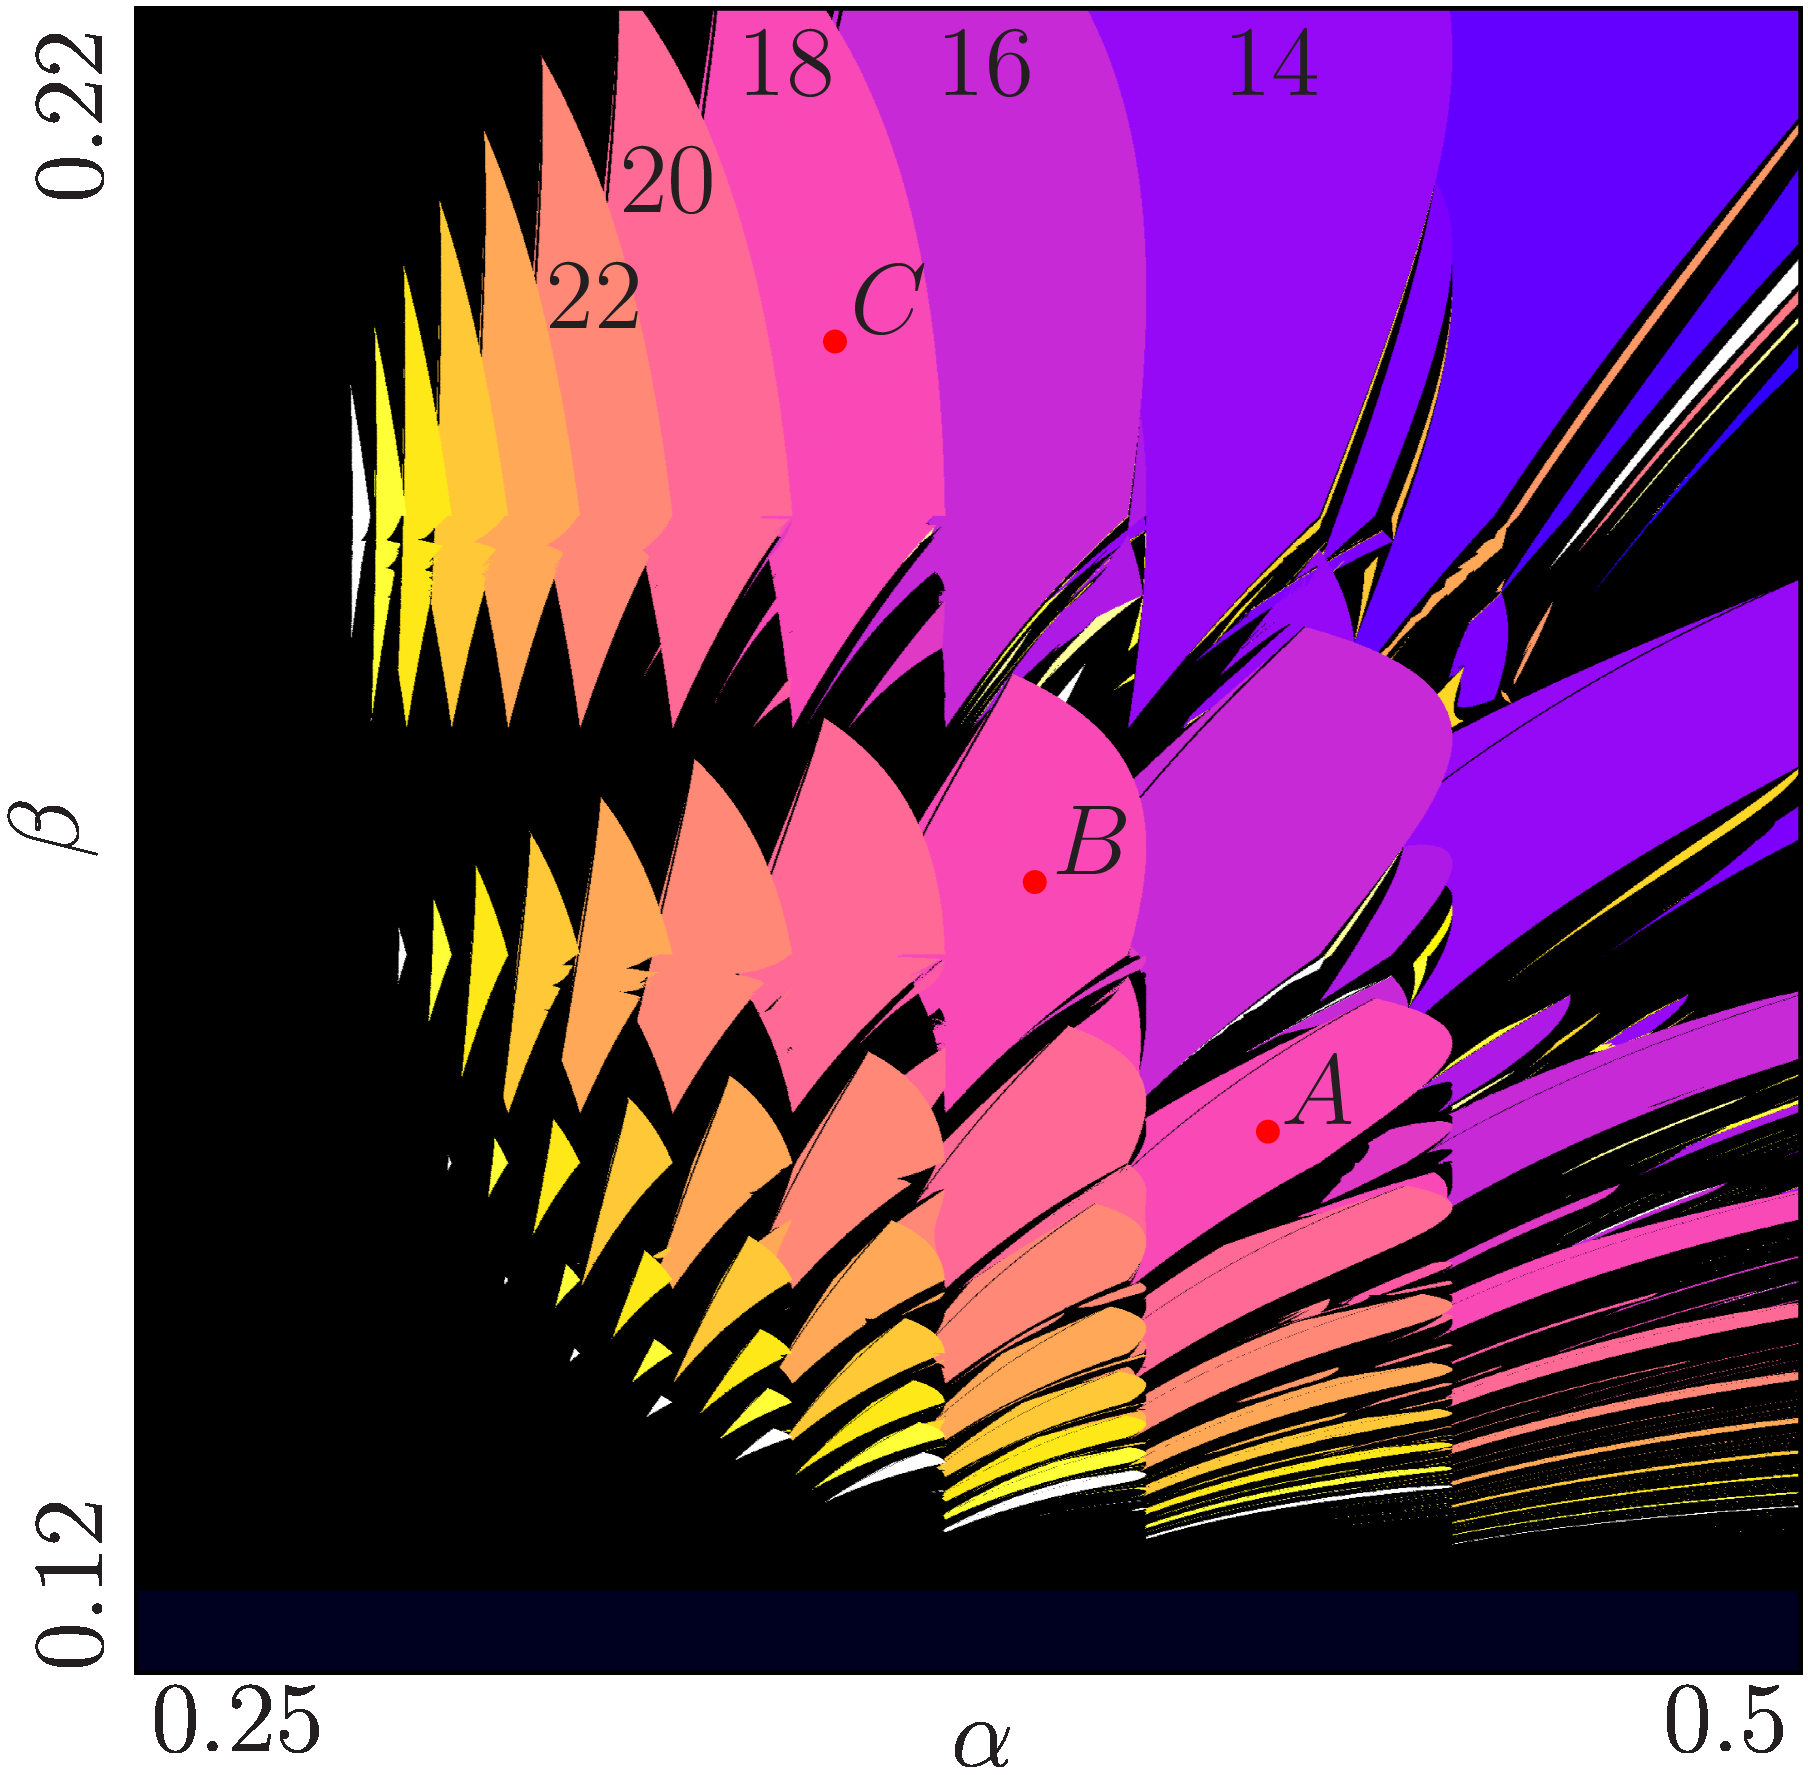
\includegraphics[width=0.6\textwidth]{../Figures/5/5.9/result.png}
	\caption[2D scan of the periods of the quadratic model with composite parameters]{
	2D scan of the periods of the piecewise quadratic model with \hl{composite} parameters $g_R\left(\frac{1}{4}\right), g_R\left(\frac{1}{2}\right),$ and $\left. \frac{d}{dx} g_R\left(x\right) \right|_{x = \frac{1}{2}}$.
	The parameters $a_L = 8, b_L = -1, g_R\left(\frac{1}{2}\right) = \frac{1}{2} + \frac{1}{40},$ and $\left. \frac{d}{dx} g_R\left(x\right) \right|_{x = \frac{1}{2}} = 1.2$ are fixed.
	The parameters $\alpha = g_R\left(\frac{1}{4}\right)$ and $\beta = c_L$ are varied in the ranges $[0.25, 0.5]$ and $[0.12, 0.22]$, respectively.
	The points $A, B,$ and $C$ mark the parameter values used for the cobweb diagrams in \Cref{fig:setup.quad.hyper.1.cobwebs}.
	Also, the numbers at the top indicate the period associated with some parameter regions.
	}
	\label{fig:setup.quad.hyper.1.period}
\end{figure}

\begin{figure}
	\centering
	\subfloat[$A$]{
		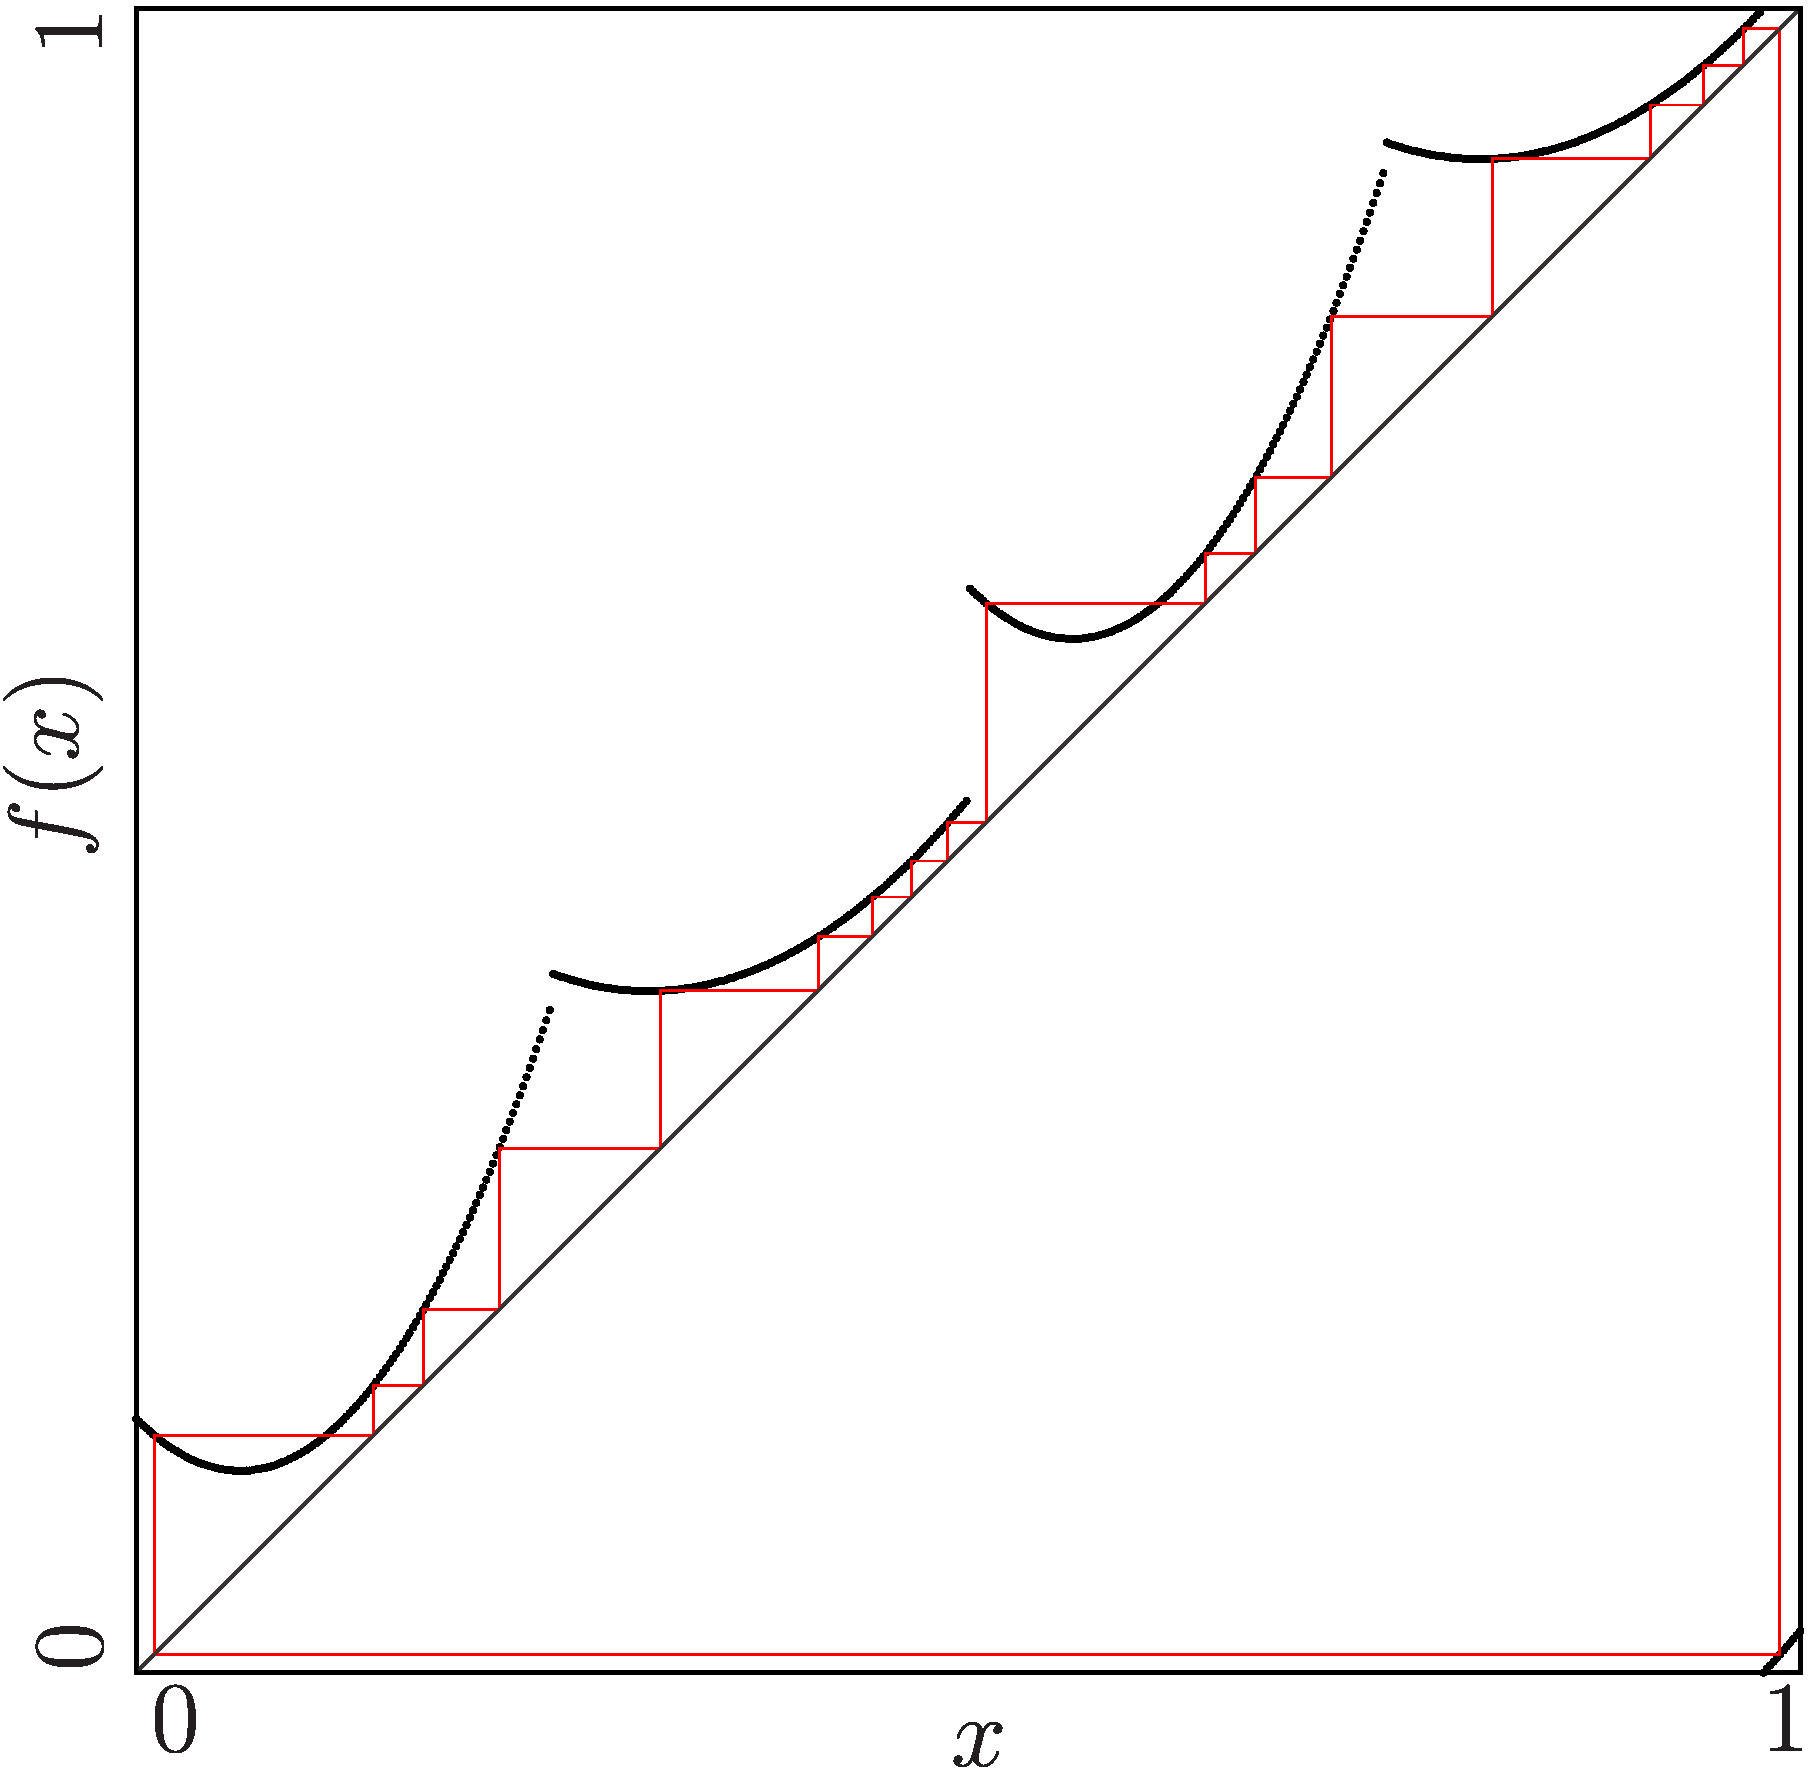
\includegraphics[width=.3 \textwidth]{../Figures/5/5.10a/result.png}
		\label{fig:setup.quad.hyper.1.cobweb.A}
	}
	\subfloat[$B$]{
		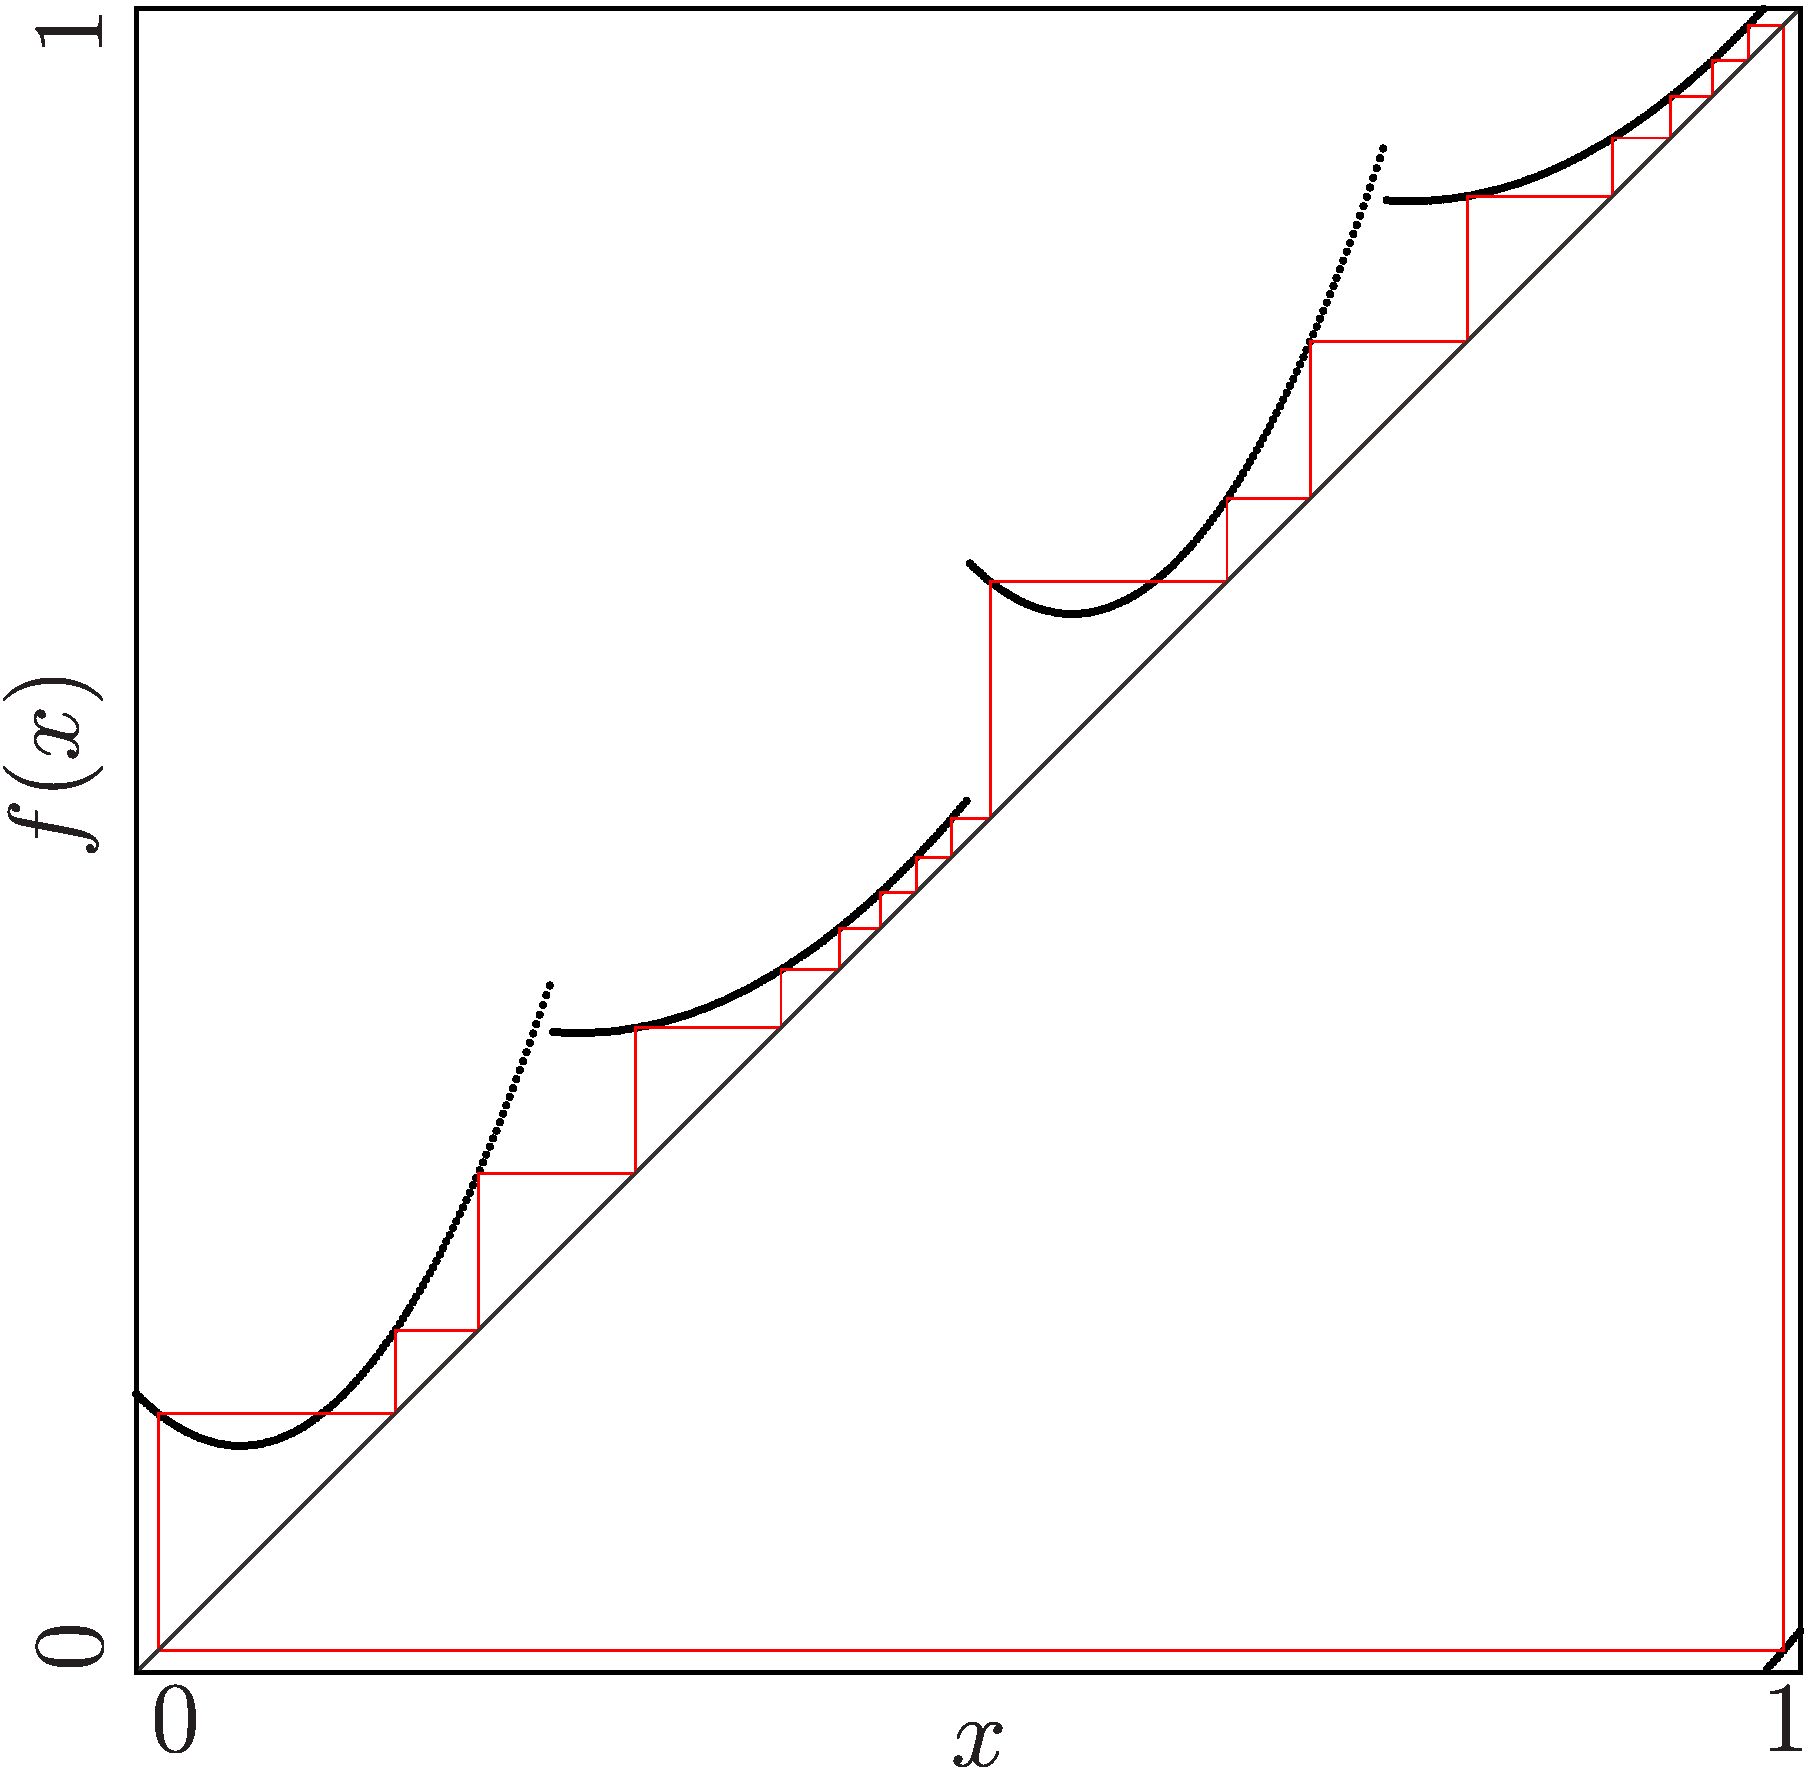
\includegraphics[width=.3 \textwidth]{../Figures/5/5.10b/result.png}
		\label{fig:setup.quad.hyper.1.cobweb.B}
	}
	\subfloat[$C$]{
		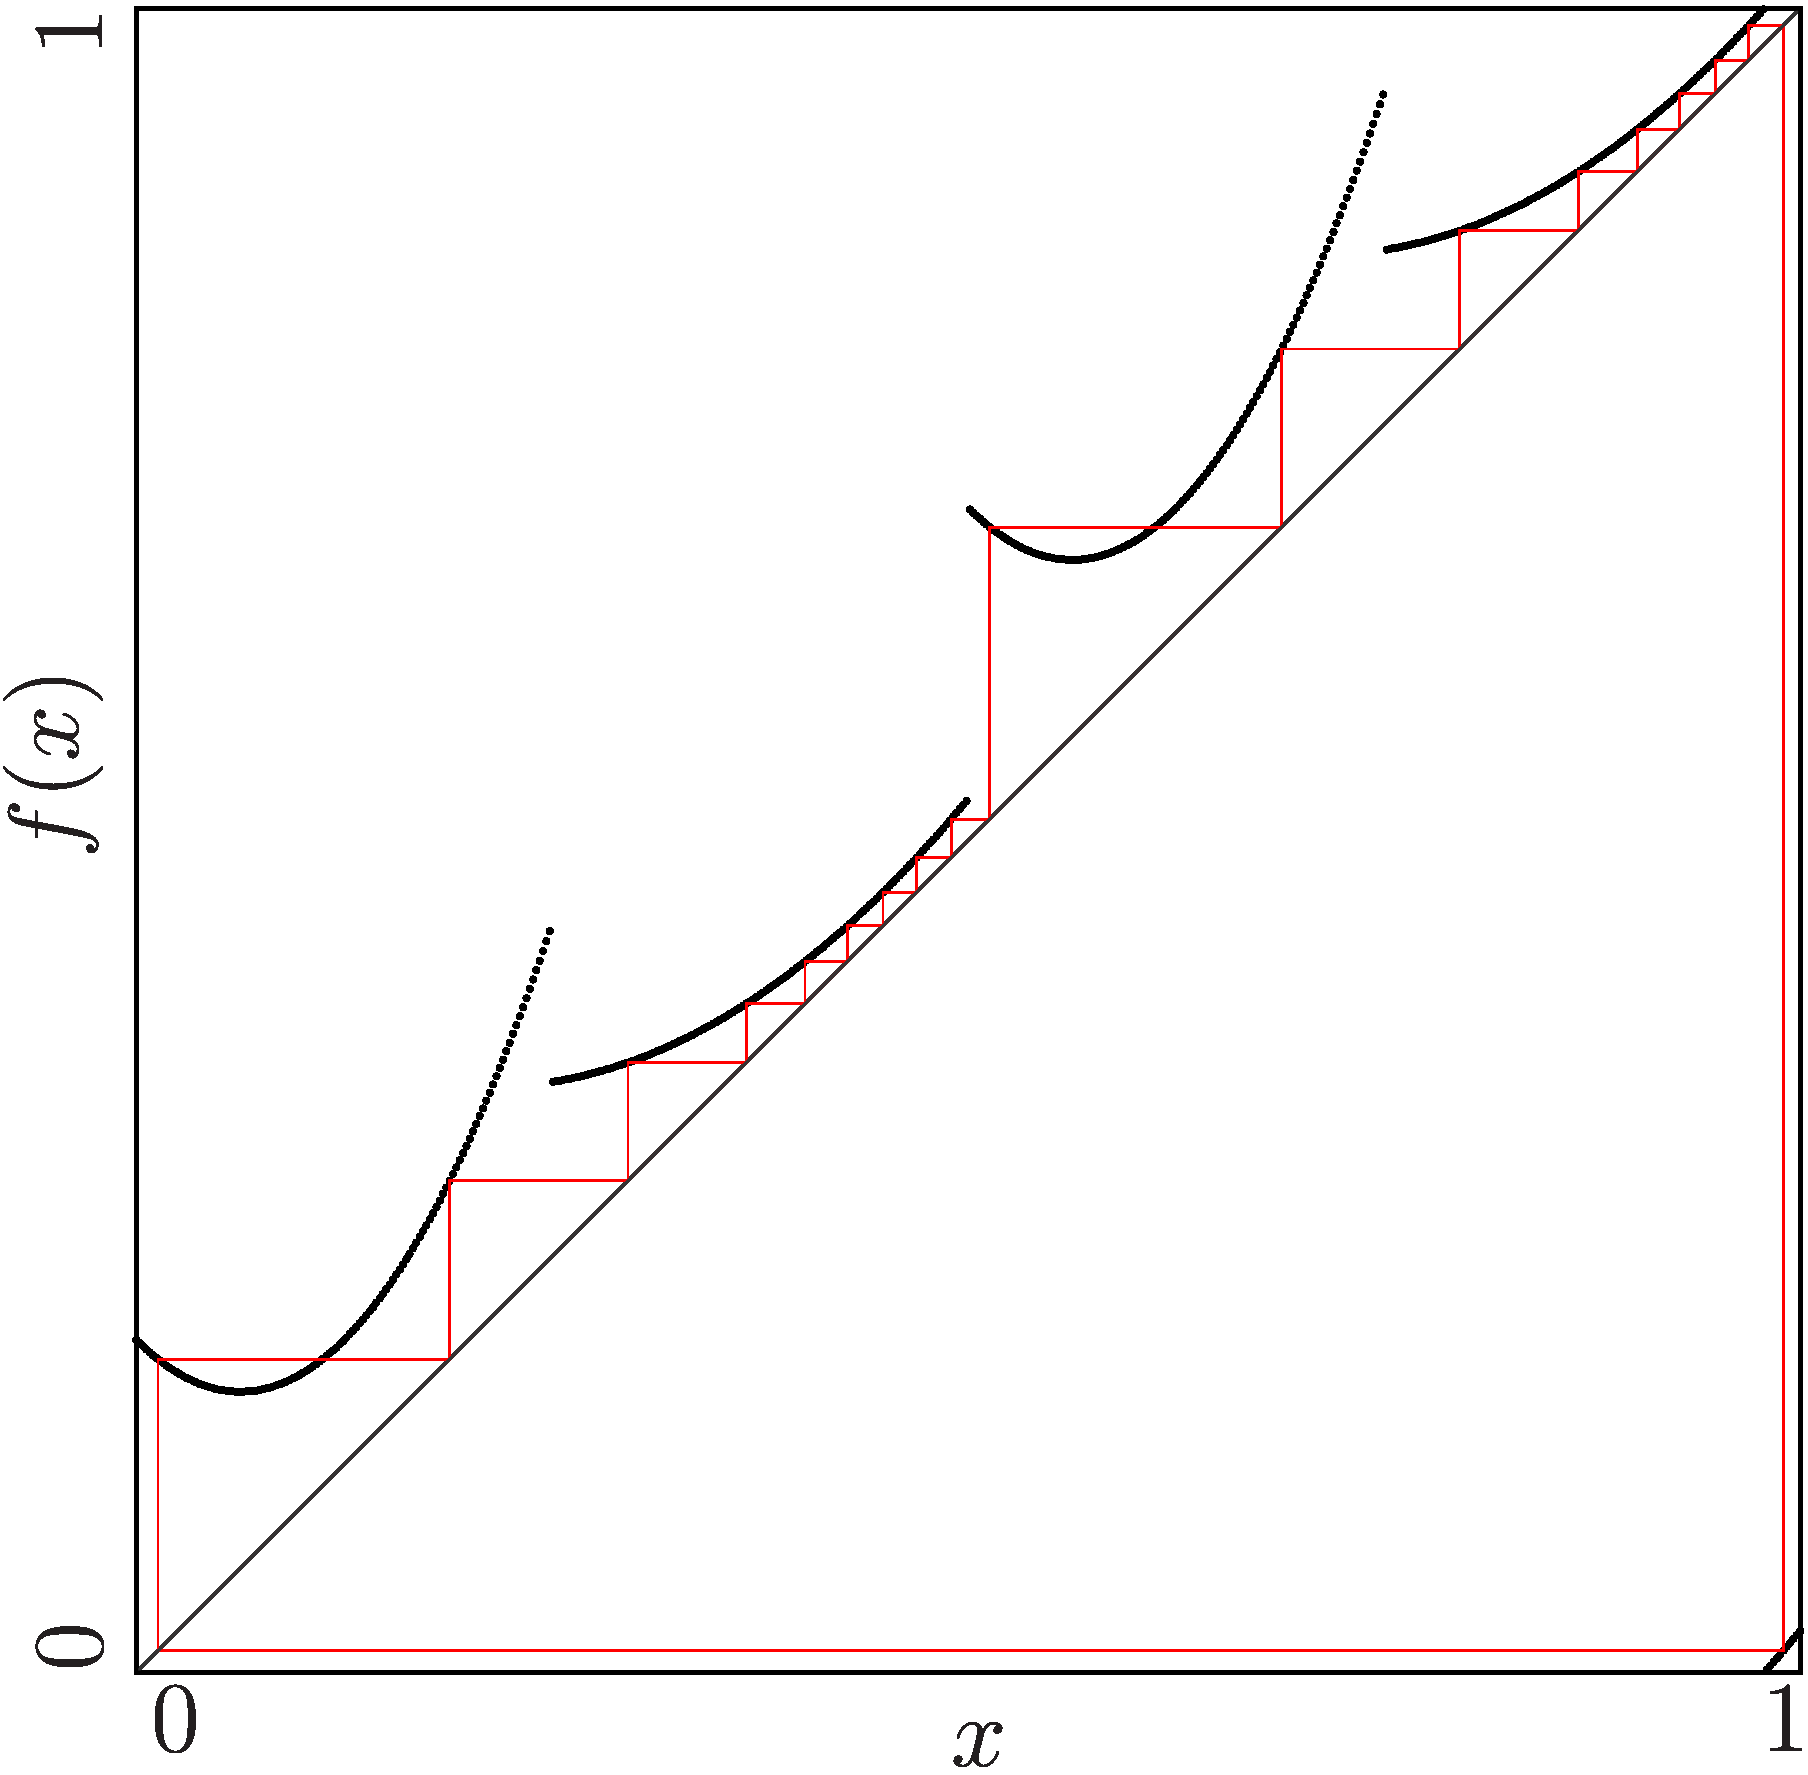
\includegraphics[width=.3 \textwidth]{../Figures/5/5.10c/result.png}
		\label{fig:setup.quad.hyper.1.cobweb.C}
	}
	\caption[Cobweb diagrams of the first piecewise quadratic model with composite parameters]{
	Cobweb diagrams at three parameter values of $\alpha = g_R\left(\frac{1}{4}\right)$ and $\beta = c_L$ in the piecewise quadratic model with hyperparameters.
	The other parameters are fixed as $a_L = 8, b_L = -1, g_R\left(\frac{1}{2}\right) = \frac{1}{2} + \frac{1}{40}$, and $\left. \frac{d}{dx} g_R(x) \right|_{x = \frac{1}{2}} = 1 + \frac{1}{5}$.
	The parameter values are marked in \Cref{fig:setup.quad.hyper.1.period}.
	(a) shows the cycle $\Cycle{\A^4\B^5\C^4\D^5}$ at the point $A$ where $\alpha = 0.42$ and $\beta = 0.1525$,
	(b) shows the cycle $\Cycle{\A^3\B^6\D^3\C^6}$ at the point $B$ where $\alpha = 0.385$ and $\beta = 0.1675$,
	and (c) shows the cycle $\Cycle{\A^2\B^7\C^2\D^7}$ at the point $C$ where $\alpha = 0.385$ and $\beta = 0.1675$.
	}
	\label{fig:setup.quad.hyper.1.cobwebs}
\end{figure}

\Cref{fig:setup.quad.hyper.1.period} shows a 2D scan of the periods associated with parameter regions in the specified parameter range for $\alpha$ and $\beta$.
At the top, some periods are annotated.
One can see that in the scan there are sequences of parameter regions that are associated with the same period.
These sequences are next to each other, where each sequence is associated with a period that is two numbers higher than the period associated with the parameter region sequence right of it.
This is similar to the \gls{pi} that can be observed in the original model, as described in \Cref{sec:state.og.dynamics}.
One difference is that the sequences in the original model were connected and formed chains.

\Cref{fig:setup.quad.hyper.1.cobwebs} shows cobweb diagrams for different parameter values along the sequence of parameter regions associated with the period $18$.
These parameter values are marked with points in \Cref{fig:setup.quad.hyper.1.period}.
\Cref{fig:setup.quad.hyper.1.cobweb.A} shows the cycle at the point $A$ with the symbolic sequence $\A^4\B^5\C^4\D^5$.
\Cref{fig:setup.quad.hyper.1.cobweb.B} shows the cycle at the point $B$ with the symbolic sequence $\A^3\B^6\C^3\D^6$.
Notice that the cycle at point $B$ has one point less on the branches $f_\A$ and $f_\C$ each than the cycle at point $A$, while it has one point more on the branches $f_\B$ and $f_\D$ each.
It is as if two points, one of each of the branches $f_\A$ and $f_\C$, moved to the next branch from one parameter region of the sequence to the next.
\Cref{fig:setup.quad.hyper.1.cobweb.C} shows the cycle at the point $B$ with the symbolic sequence $\A^2\B^7\C^3\D^7$.
Again, two points, one of each of the branches $f_\A$ and $f_\C$, moved to the next branch from the parameter region with point $B$ to the parameter region with the point $C$.
This is also very similar to the behavior of the original model, where two points, one of each of the branches $F_\A$ and $F_\C$, moved to the next branch each along the chain of parameter regions associated with the same period, as described in \Cref{sec:state.og.dynamics}.
Besides that the sequences of parameter region associated with the same period are not connected here, there is another difference to the behavior of the original model.
In the original model there are ``type B'' parameter regions between the ``type A'' parameter regions of a chain of parameter regions with the same period.
To reiterate, ``type A'' parameter regions are associated with a single symmetric cycle.
These are the parameter regions, one can observe in this case also.
Between two ``type A'' parameter regions there is a parameter region that is associated with two coexisting asymmetrical twin cycles, called ``type B'' parameter regions.
These ``type B'' parameter regions are missing in this case.

\subsection{Shallow Parabola-shaped Branches $f_\A$ and $f_\C$}
\label{sec:setup.quad.hyper.2}

To close the gaps in between the parameter regions in the sequences, the parameters of the function $g_L$ that governs the shape of the branches $f_\A$ and $f_\C$ is adjusted.
The new fixed parameter values are $a_L = 4$ and $b_L = -\frac{1}{2}$.
And the other fixed parameters stay the same as in the previous section.

One can see in \Cref{fig:setup.quad.hyper.1.cobwebs} that the shape of the branches $f_\A$ and $f_\C$ is very steep.
This is different from the branches $F_\A$ and $F_\C$ in the original model that were more shallow.
The new fixed parameter values of $a_L$ and $b_L$ also cause the shape of the branches $f_\A$ and $f_\C$ to be more shallow.
One can see this in the cobweb diagrams in \Cref{fig:setup.quad.hyper.2.cobwebs}.
The varied parameters are the same as in the previous section and therefore the parameter effects of $E_0$ and $\chi_0$ on the original model function are emulated well.
This was thoroughly described in the previous section, \Cref{sec:setup.quad.hyper.1}.

\Cref{fig:setup.quad.hyper.2.period} shows 2D scans of periods associated with parameter regions in this model.
It shows 2 different versions of scans in the same parameter range, $\alpha \in [0.275, 0.35]$ and $\beta \in [0.15, 0.1875]$.
The first scan in \Cref{fig:setup.quad.hyper.2.period.full} shows the periods of the model as we have seen it also in the previous sections.
The second scan in \Cref{fig:setup.quad.hyper.2.period.halved} shows the periods of the same model but halved.
This reveals ``type B'' parameter regions as they are associated with higher periods than the ``type A'' parameter regions of the same chains in the halved model.
The reason for this is covered in-depth in \Cref{sec:add.add.halved}, but for now only the fact that it reveals ``type B'' parameter regions is important.

We can see in \Cref{fig:setup.quad.hyper.2.period.full}, that the gap between the ``type A'' parameter regions of a sequence of parameter regions associated with the same period closed.
Also, there are sections of the chains where they get narrower, for example at point $C$.
In the original model one can observe the same narrowing of the chains.
These narrower sections are ``type B'' parameter regions in the original model.


\Cref{fig:setup.quad.hyper.2.period.halved} reveals ``type B'' parameter regions in the quadratic model with compound parameters.
We can see that ``type A'' and ``type B'' parameter regions alternate in the chains of parameter regions associated with the same period.
Also, the ``type B'' parameter regions are at the narrower sections of the chains.
This is exactly the same behavior one can observe in the original model when examining the types of the parameter regions making up the chains and their arrangement.

The period the chains are associated with also still increments in neighboring chains as was observed in the last section, \Cref{sec:setup.quad.hyper.1}.
Therefore, this structure is similar to the \gls{pi} structure one can observe in the original model when looking at the periods associated with parameter regions and their types.
But this is not the only characteristic of cycles.
Therefore, the symbolic sequences of the cycles associated with the parameter regions making up the chains are analyzed next.

\begin{figure}
	\centering
	\subfloat[Model]{
		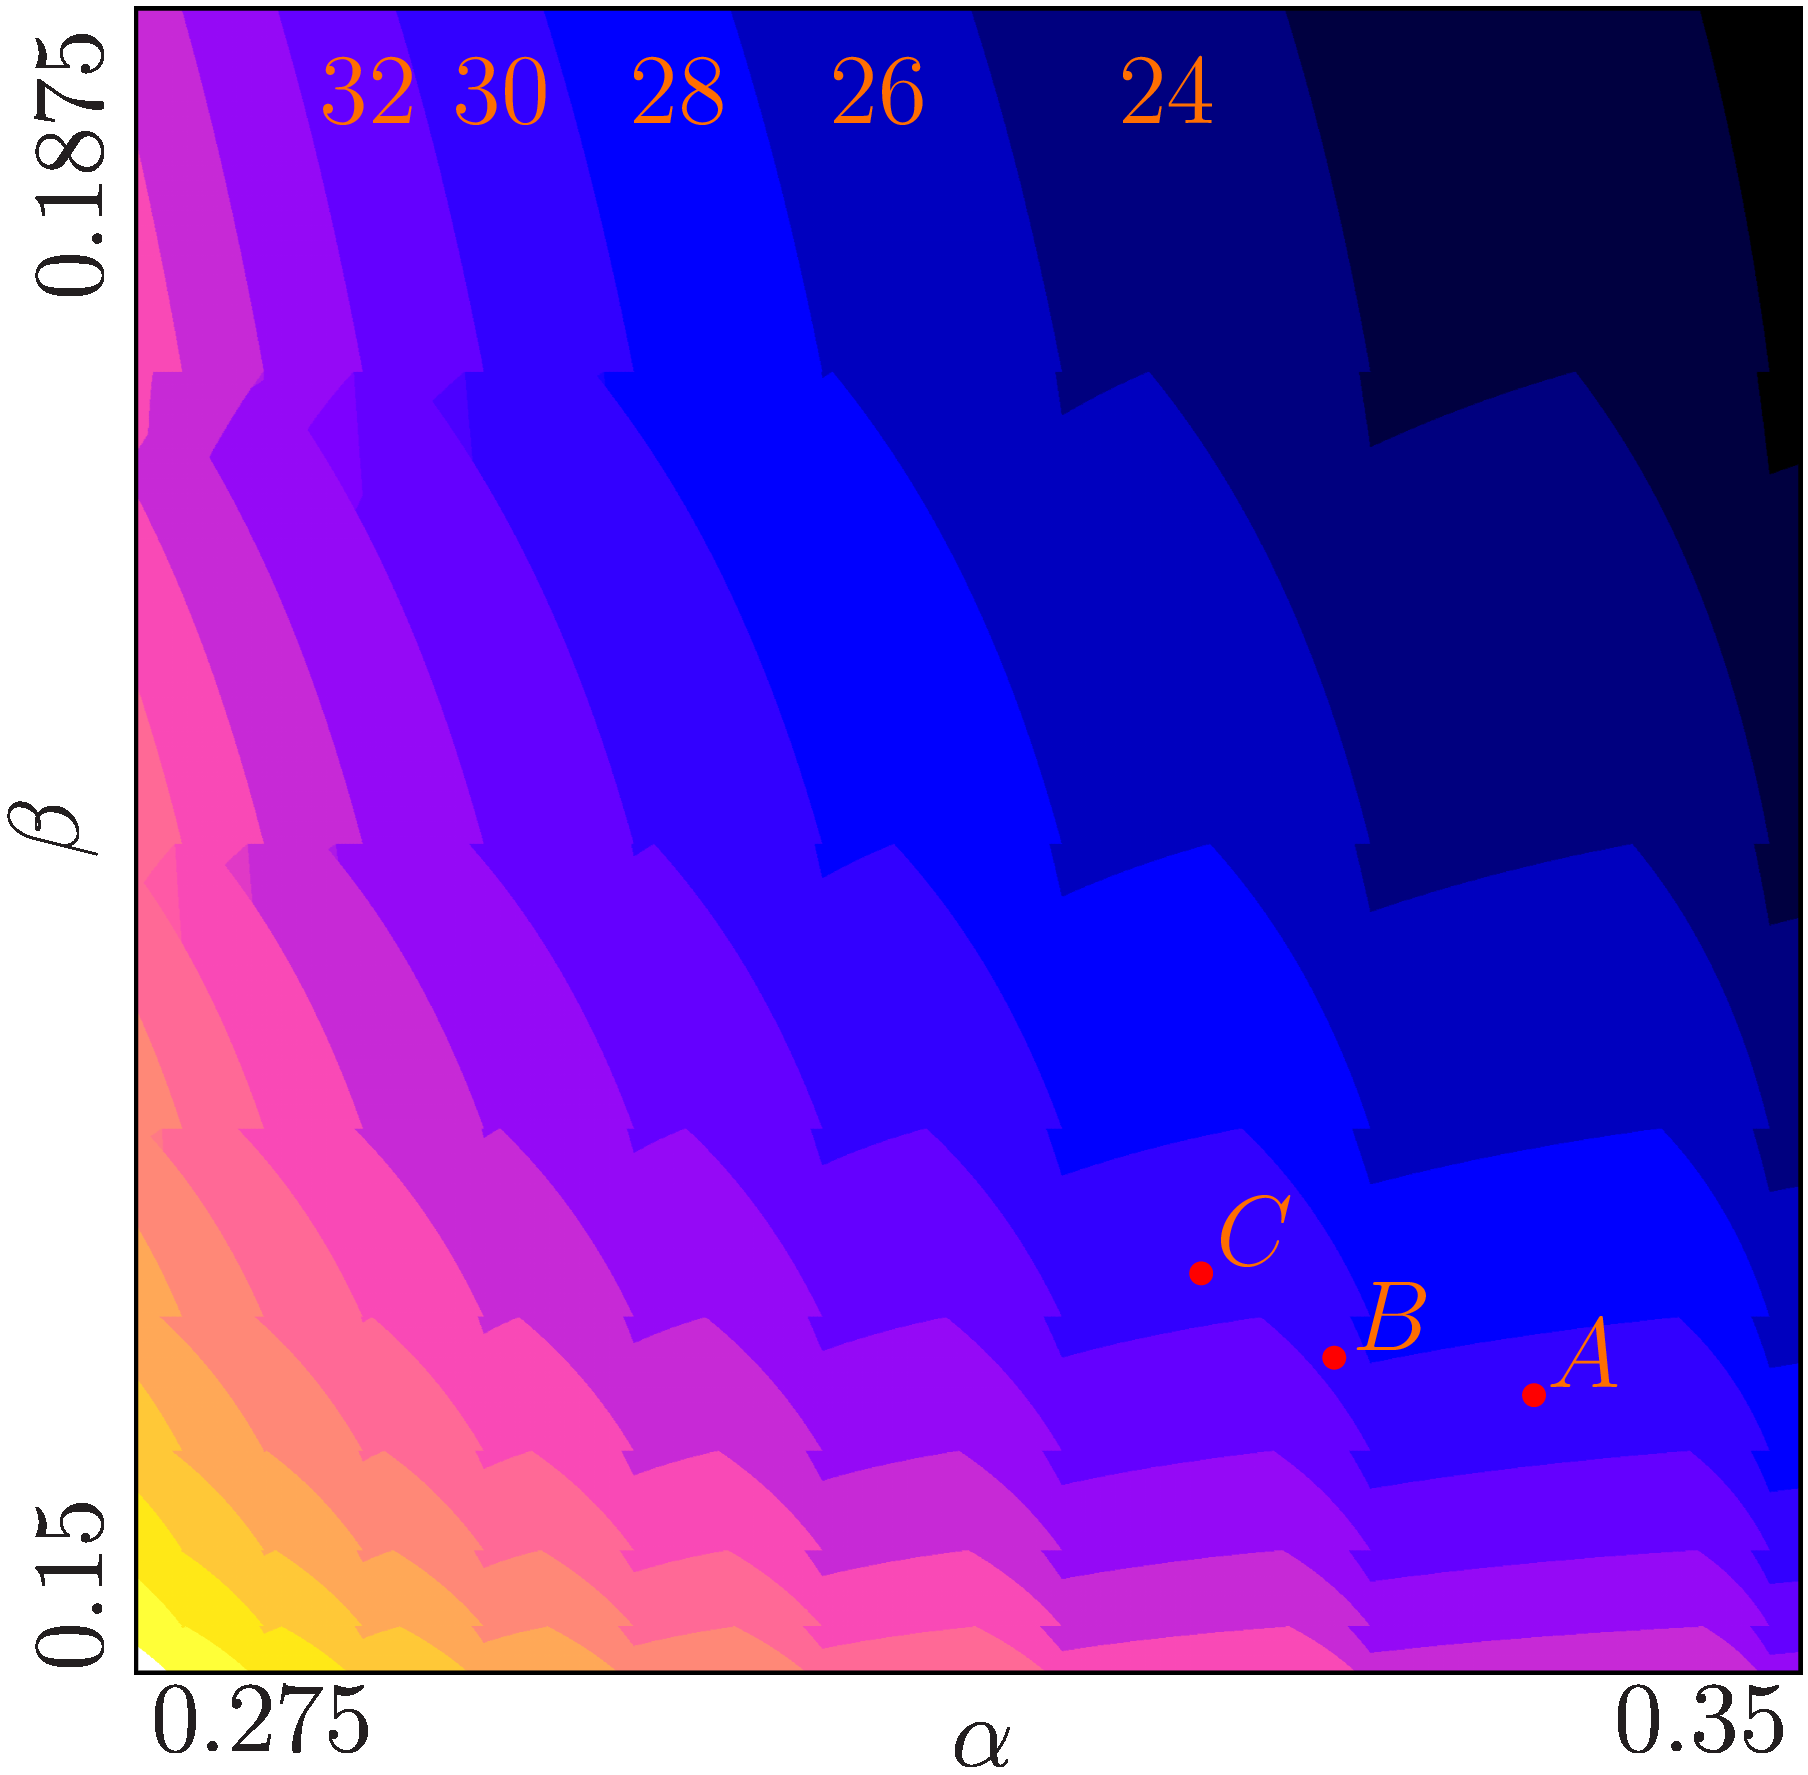
\includegraphics[width=.48 \textwidth]{../Figures/5/5.11a/result.png}
		\label{fig:setup.quad.hyper.2.period.full}
	}
	\subfloat[Halved model]{
		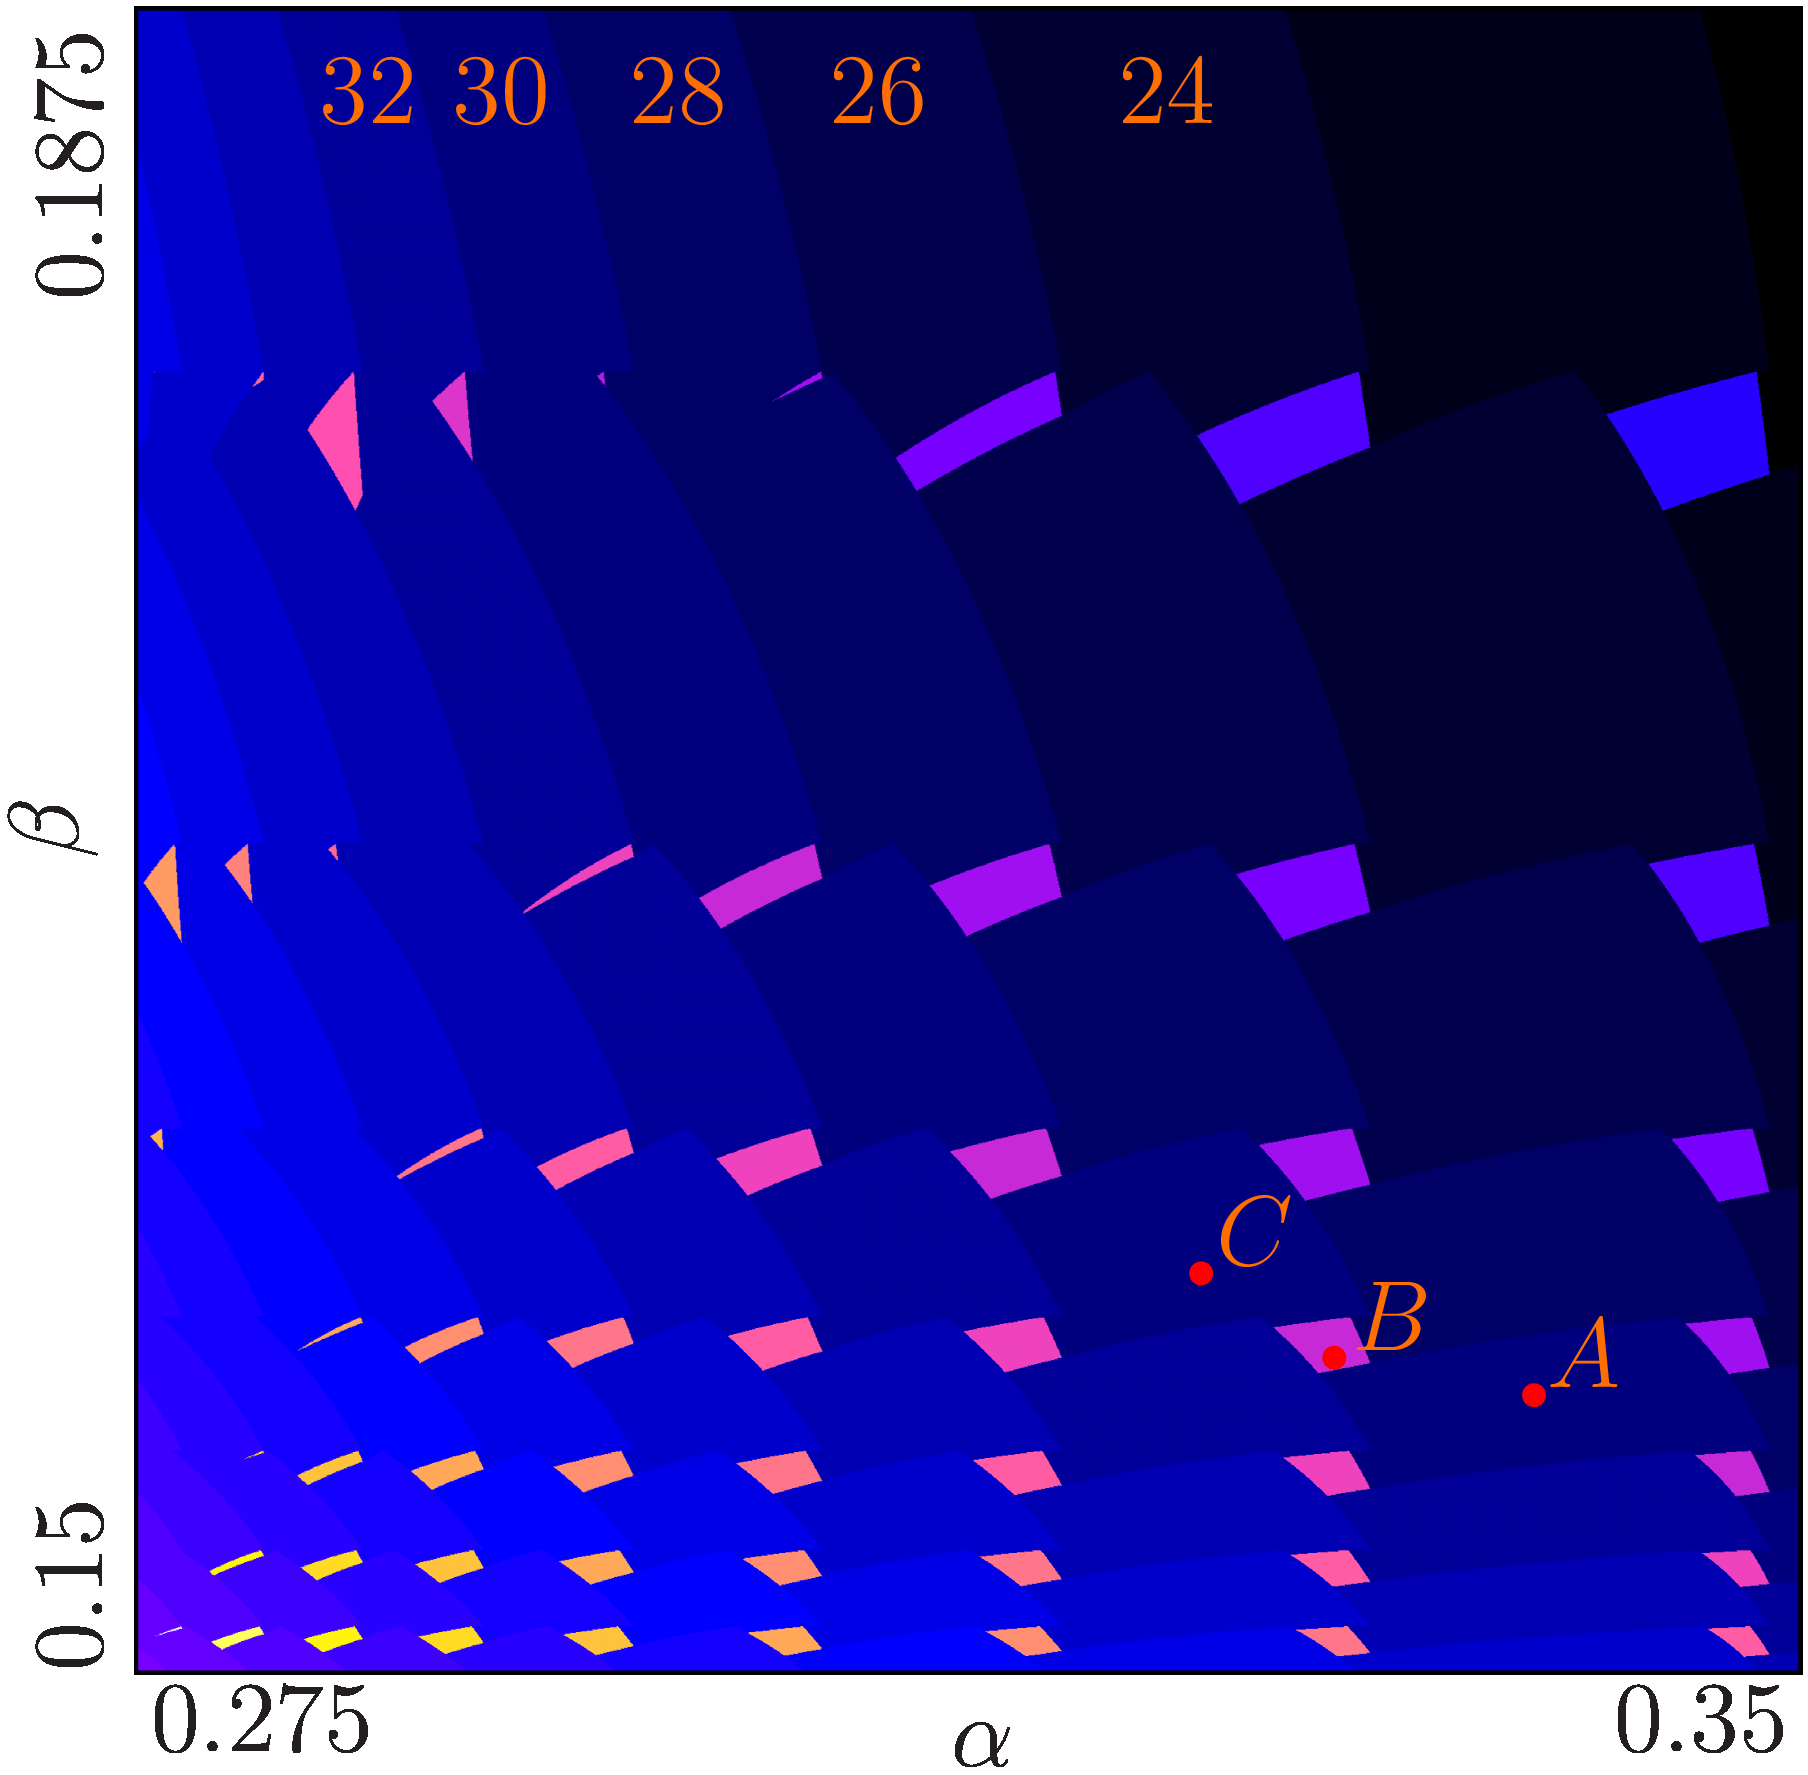
\includegraphics[width=.48\textwidth]{../Figures/5/5.11b/result.png}
		\label{fig:setup.quad.hyper.2.period.halved}
	}
	\caption[2D scan of the periods of the quadratic model with hyperparameters for different values of the fixed parameters]{
	2D scan of the periods of the piecewise quadratic model with hyperparameters $g_R\left(\frac{1}{4}\right), g_R\left(\frac{1}{2}\right),$ and $\left. \frac{d}{dx} g_R\left(x\right) \right|_{x = \frac{1}{2}}$.
	The parameters $a_L = 4, b_L = -\frac{1}{2}, g_R\left(\frac{1}{2}\right) = \frac{1}{2} + \frac{1}{40},$ and $\left. \frac{d}{dx} g_R\left(x\right) \right|_{x = \frac{1}{2}} = 1.2$ are fixed.
	The parameters $\alpha = g_R\left(\frac{1}{4}\right)$ and $\beta = c_L$ are varied in the ranges $[0.275, 0.35]$ and $[0.15, 0.1875]$, respectively.
	The points $A, B,$ and $C$ mark the parameter values used for the cobweb diagrams in \Cref{fig:setup.quad.hyper.2.cobwebs}.
	Also, the numbers at the top indicate the period of the parameter region chains.
	(a) shows the scan for the model as defined above, while (b) shows the scan for the halved model where we can see ``type B'' parameter regions as they have higher periods than the ``type A'' parameter regions of the same chain.
	}
	\label{fig:setup.quad.hyper.2.period}
\end{figure}

\begin{figure}
	\centering
	\subfloat[$A$]{
		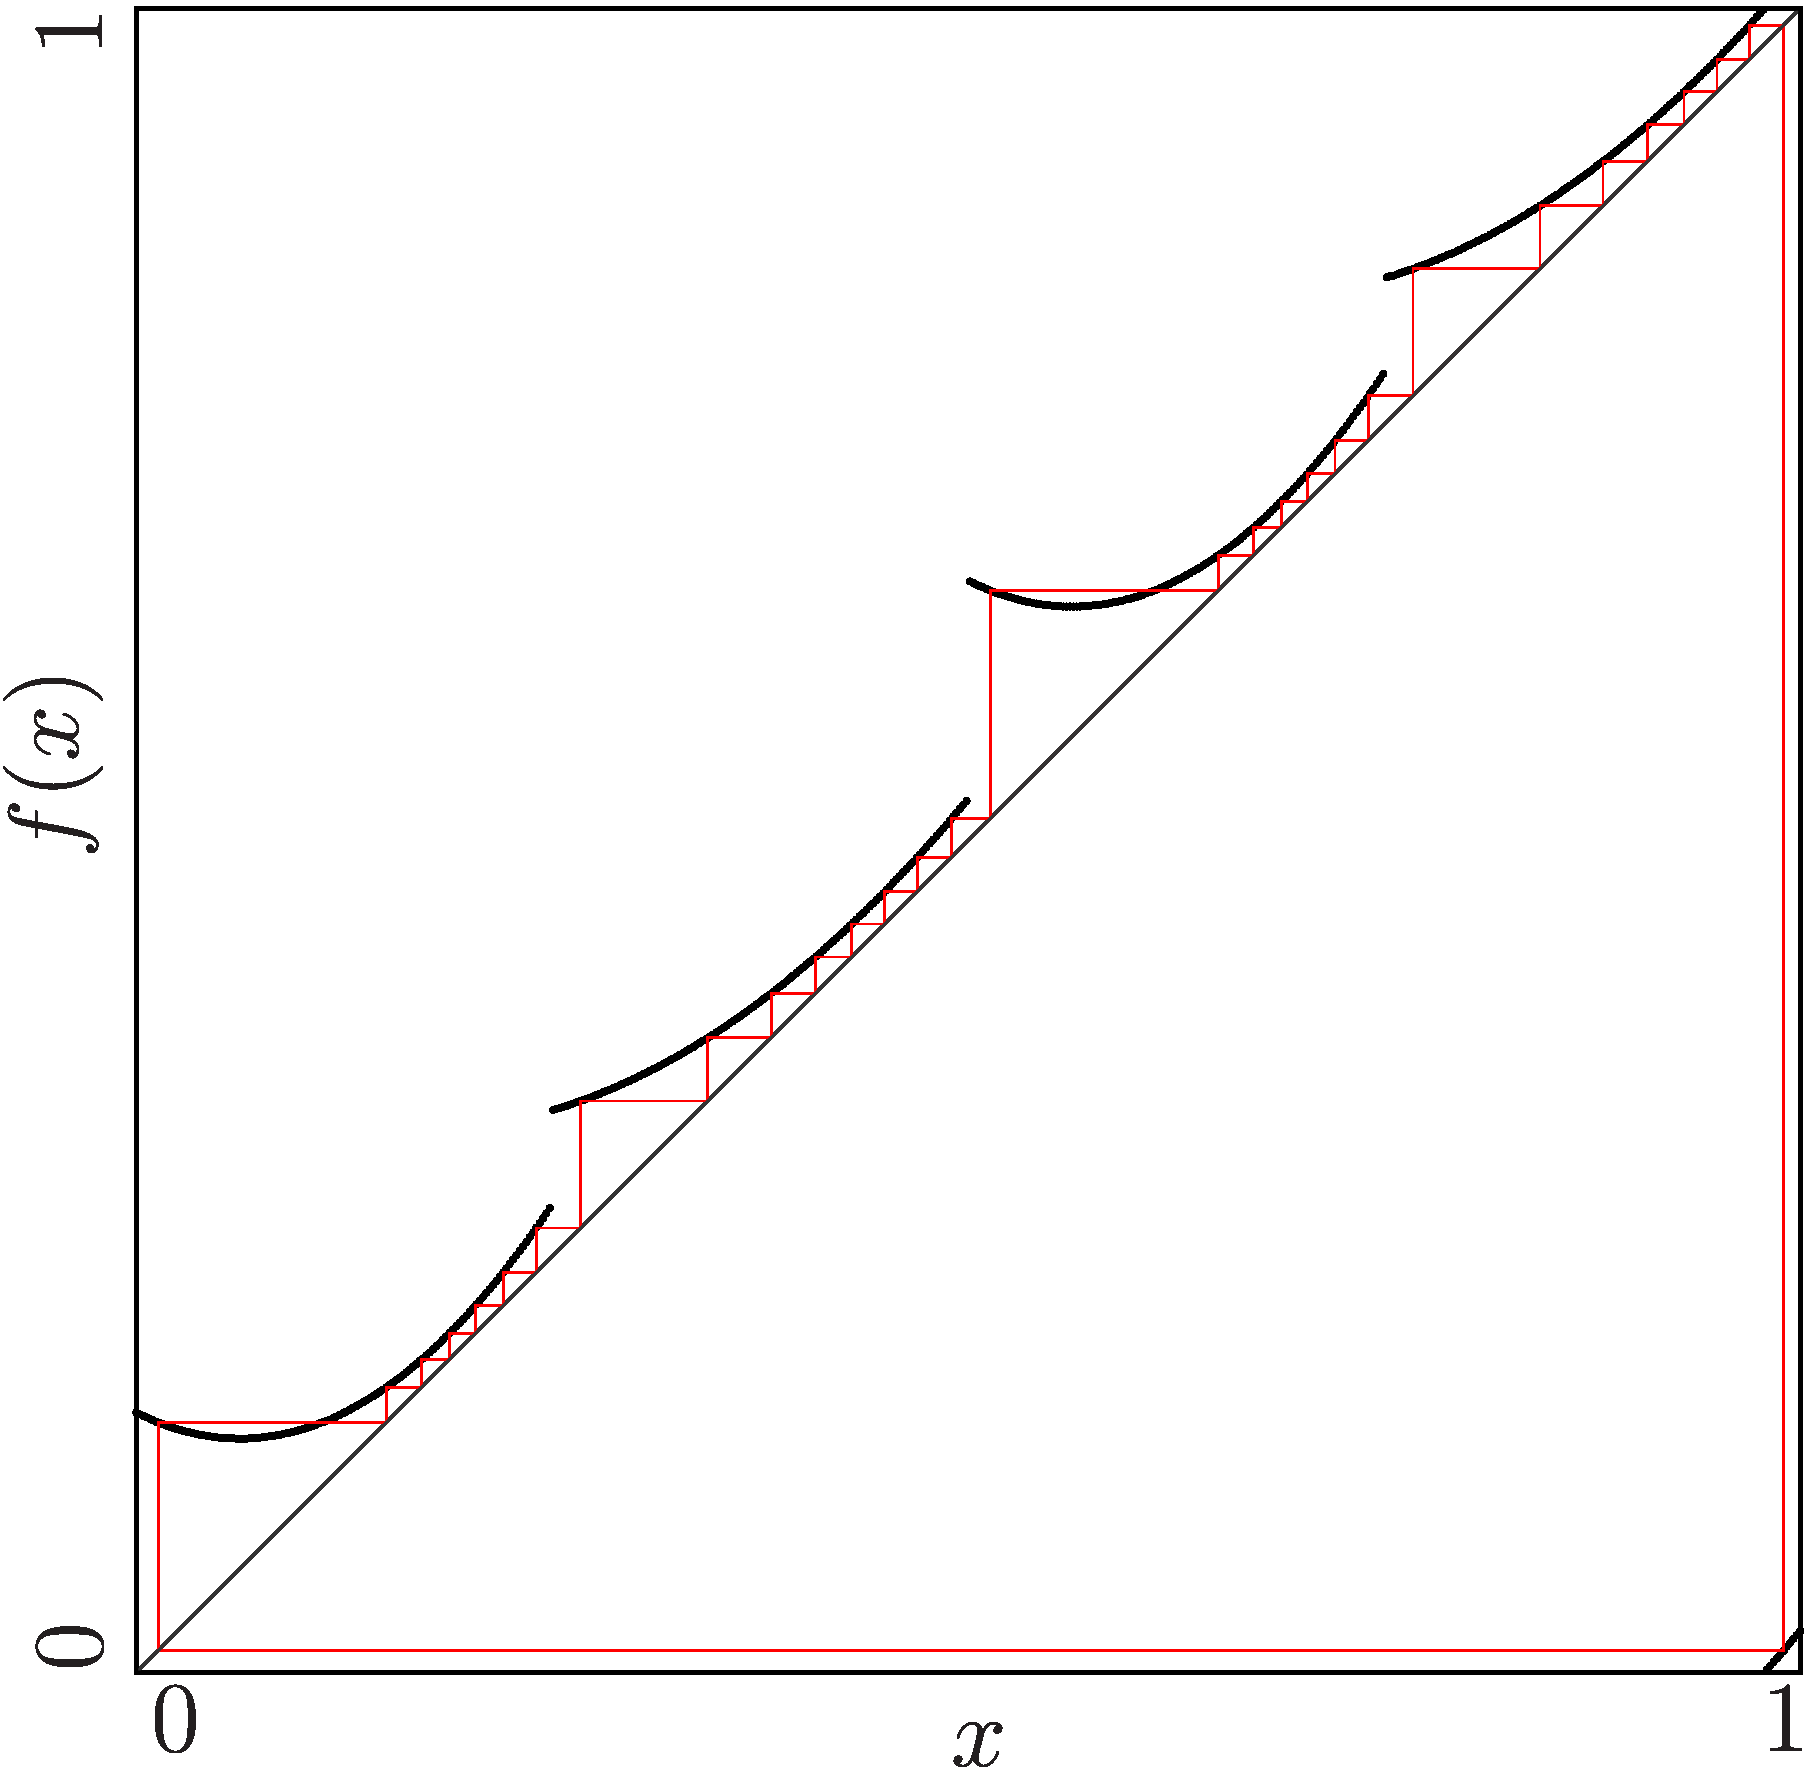
\includegraphics[width=.3 \textwidth]{../Figures/5/5.12a/result.png}
		\label{fig:setup.quad.hyper.2.cobweb.A}
	}
	\subfloat[$B$]{
		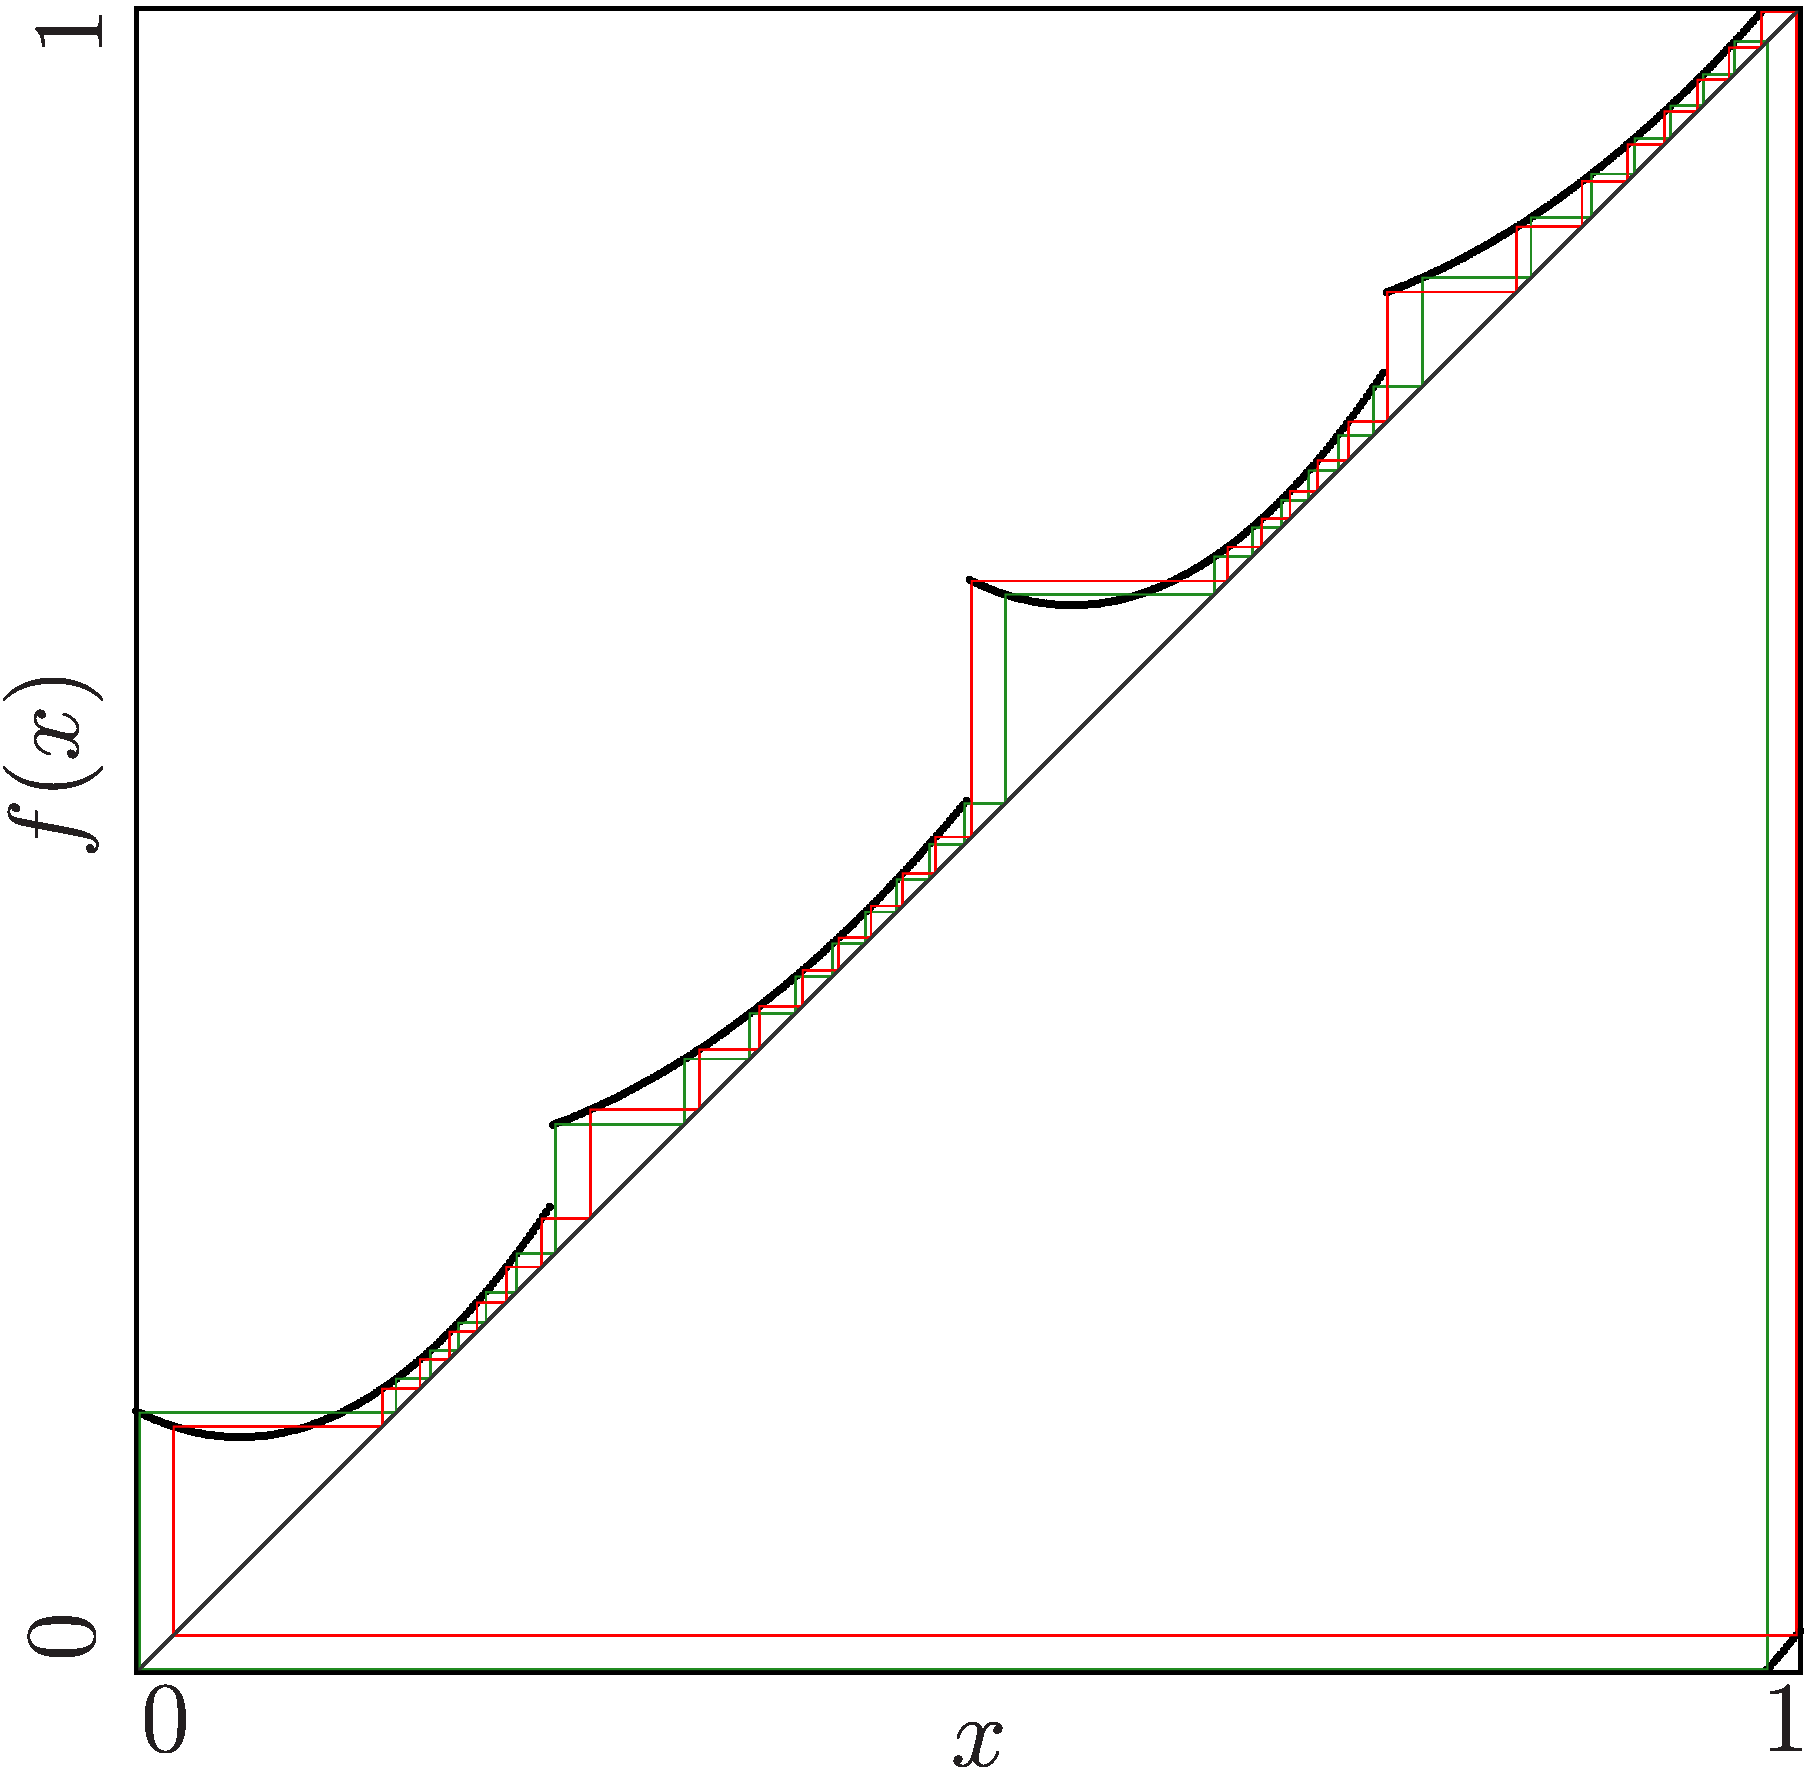
\includegraphics[width=.3 \textwidth]{../Figures/5/5.12b/result.png}
		\label{fig:setup.quad.hyper.2.cobweb.B}
	}
	\subfloat[$C$]{
		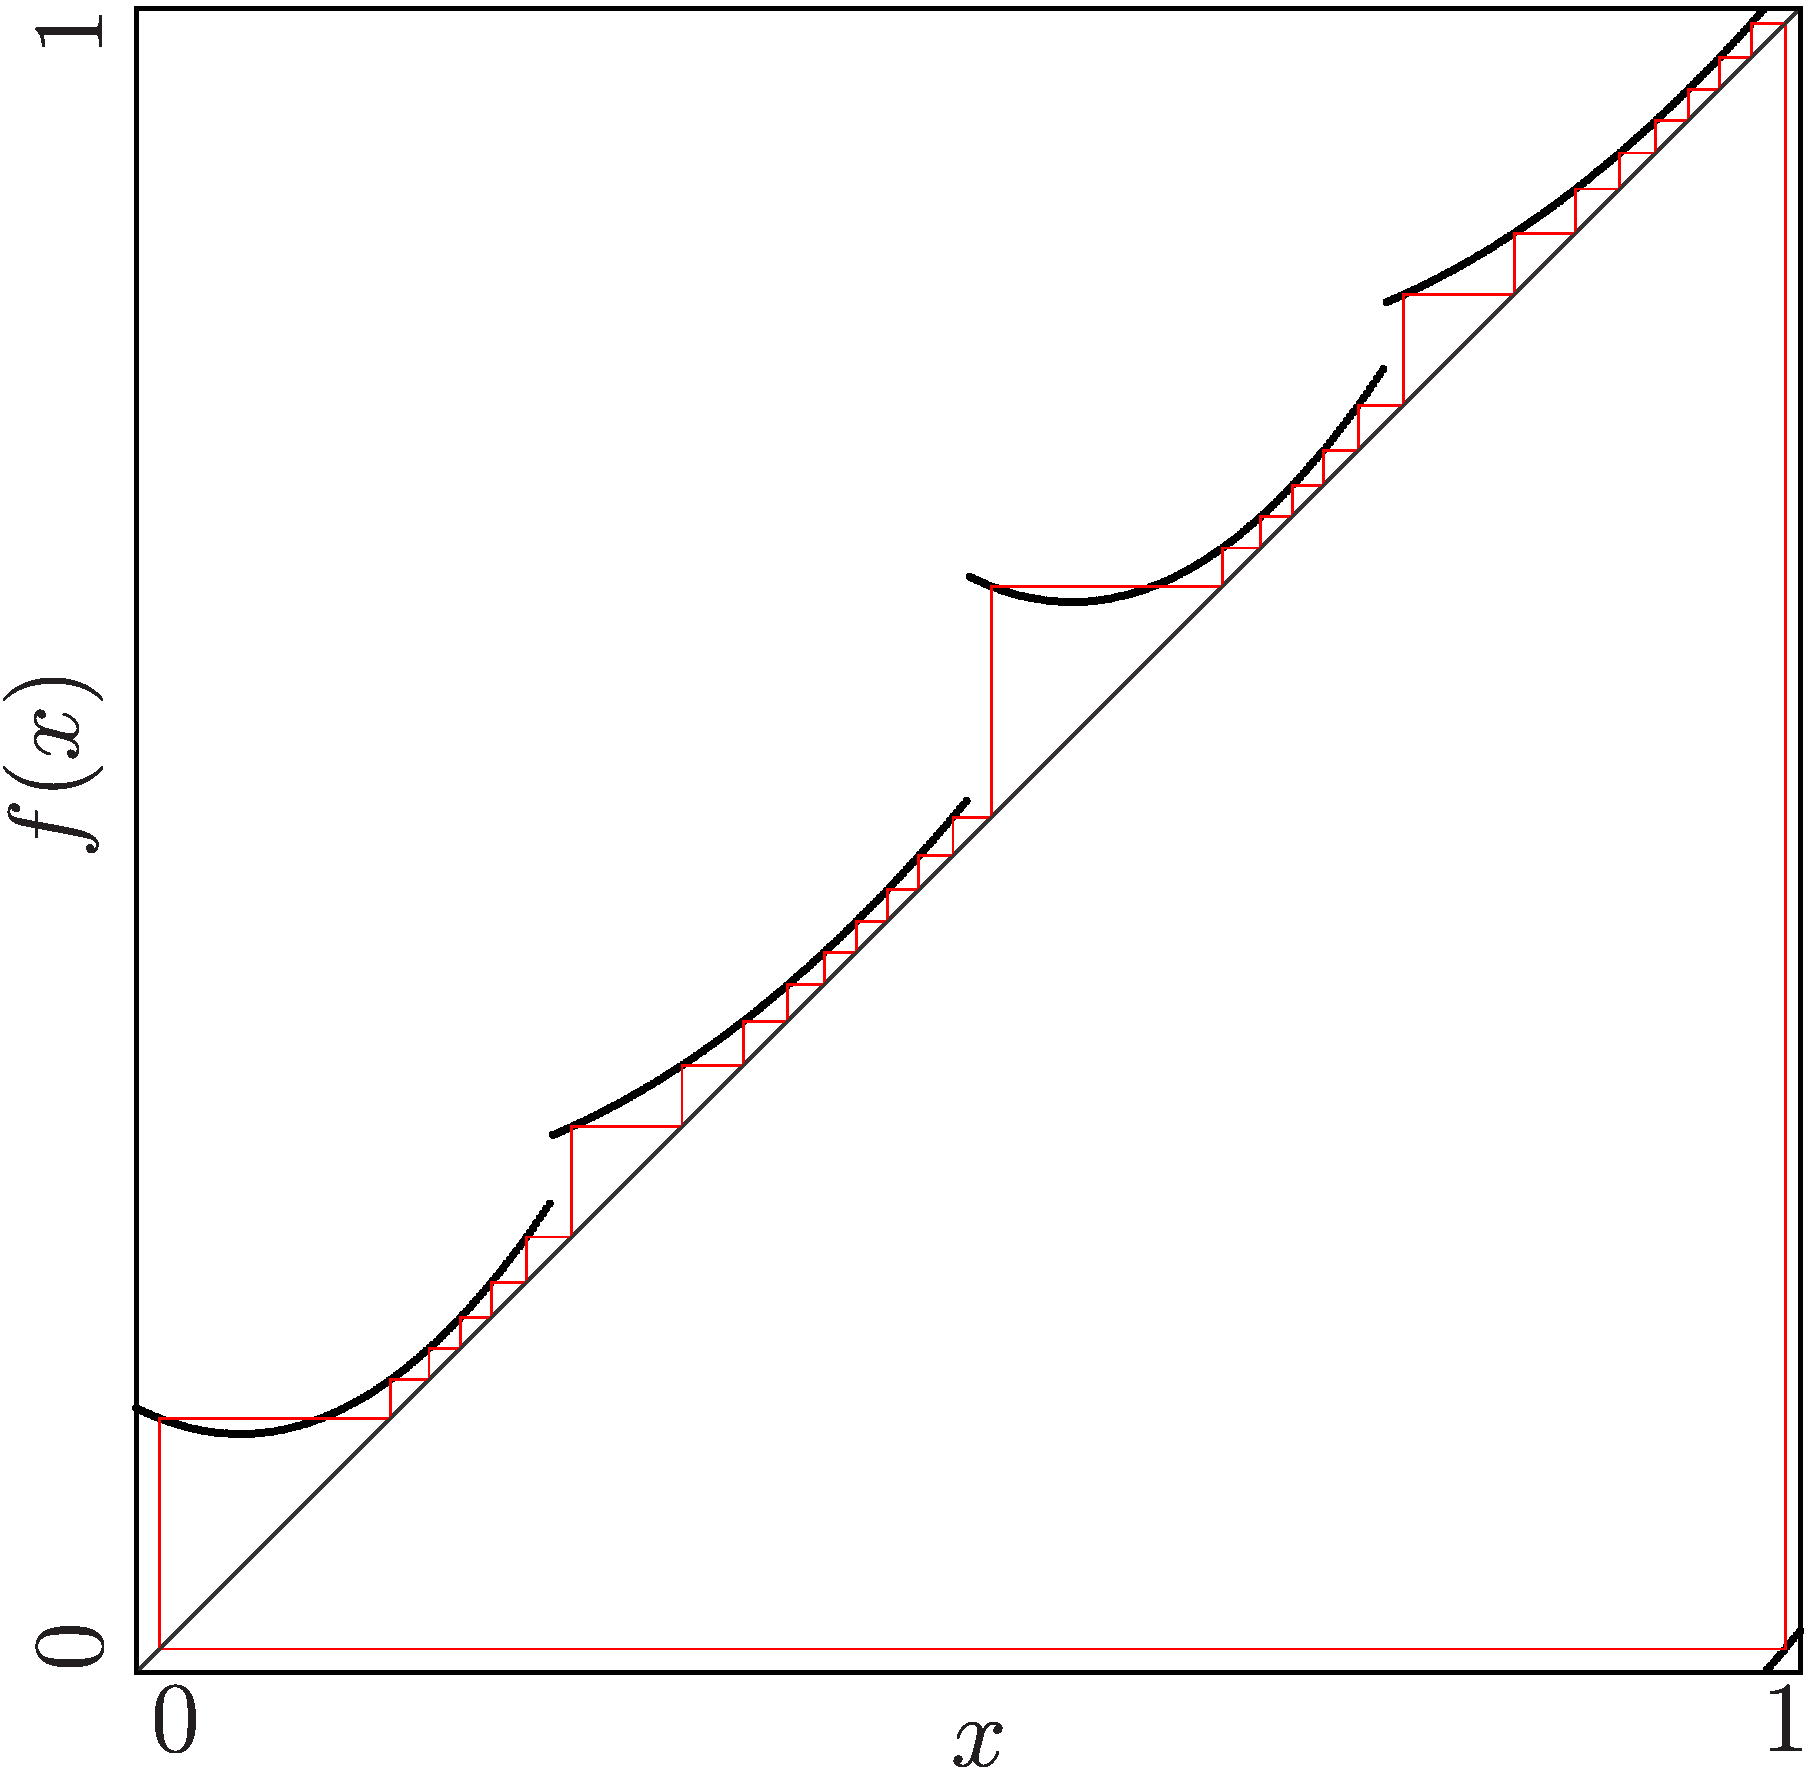
\includegraphics[width=.3 \textwidth]{../Figures/5/5.12c/result.png}
		\label{fig:setup.quad.hyper.2.cobweb.C}
	}
	\caption[Cobwebs of the piecewise quadratic model with hyperparameters for different values of the fixed parameters]{
	Cobweb diagrams at three parameter values of $\alpha = g_R\left(\frac{1}{4}\right)$ and $\beta = c_L$ in the piecewise quadratic model with hyperparameters.
	The other parameters are fixed as $a_L = 4, b_L = -\frac{1}{2}, g_R\left(\frac{1}{2}\right) = \frac{1}{2} + \frac{1}{40}$, and $\left. \frac{d}{dx} g_R(x) \right|_{x = \frac{1}{2}} = 1 + \frac{1}{5}$.
	The parameter values are marked in \Cref{fig:setup.quad.hyper.2.period}.
	(a) shows the cycle $\Cycle{\A^7\B^8\C^7\D^8}$ the at point $A$where $\alpha = 0.338$ and $\beta = 0.15625$,
	(b) shows the two coexisting cycles $\Cycle{\A^7\B^8\C^7\D^8}$ (green) and $\Cycle{\A^6\B^9\C^6\D^9}$ (red) at the point $B$where $\alpha = 0.329$ and $\beta = 0.1571$,
	and (c) shows the cycle $\Cycle{\A^6\B^9\C^6\D^9}$ at the point $C$where $\alpha = 0.323$ and $\beta = 0.159$.
	}
	\label{fig:setup.quad.hyper.2.cobwebs}
\end{figure}

\Cref{fig:setup.quad.hyper.2.cobwebs} contains the cobweb diagrams for the cycles at the parameter values that are marked with points $A, B,$ and $C$ in \Cref{fig:setup.quad.hyper.2.period}.
This chain of parameter regions is associated with the period $30$, therefore all the cycles shown here also have the period $30$.
The symbolic sequence of the cycle at point $A$ is $\A^7\B^8\C^7\D^8$.
It is a symmetric cycle and therefore the parameter region is of ``type A''.
The symbolic sequence of the cycle at point $C$ is $\A^6\B^9\C^6\D^9$.
It is also a symmetric cycle and this parameter region is also of ``type A''.
The parameter region with point $C$ is the next ``type A'' parameter region after the parameter region with point $A$ in the chain.
And just like in the original model, one point of each of the branches $f_\A$ and $f_\C$ moved to the next branch.

Between those two ``type A'' parameter regions there is a narrower ``type B'' parameter region with the same period.
It is marked with the point $C$.
At this point, there are 2 coexisting cycles with the period 30.
Their symbolic sequences are $\A^7\B^8\C^6\D^9$ and $\A^6\B^9\C^7\D^8$, respectively.
This is exactly the same behavior that one can observe in the original model.
Between two ``type A'' parameter regions with the cycles $\Cycle{\A^a\B^b\C^c\D^d}$ and $\Cycle{\A^c\B^d\C^c\D^d}$ there is a ``type B'' parameter region with the two coexisting cycles $\Cycle{\A^a\B^b\C^c\D^d}$ and $\Cycle{\A^c\B^d\C^c\D^d}$.
Where $c = a - 1$ and $d = b + 1$.

Therefore, the bifurcation structure in this model fulfills all criteria, although it is mirrored.
In the \gls{pi} structure in the original model, the periods increased from left to right, here they increase from right to left.
Also, the chains start in the lower left corner and go towards to the upper right corner, here they start in the lower right corner and go towards the upper left corner.
But the model can still be simplified.
The branches $f_\B$ and $f_\D$ are only increasing and almost linear.
One can observe this in the cobweb diagrams in \Cref{fig:setup.quad.hyper.2.cobwebs}.


\section{Piecewise Hybrid Quadratic Model with Hyperparameters}
\label{sec:setup.quad.hybrid}

When looking at the cobweb diagrams in \Cref{fig:setup.quad.hyper.2.cobwebs}, one can see that the branches $f_\B$ and $f_\D$ are mostly monotonous.
Even when the branches are not, the stable cycles at these points only have points on the monotonously increasing part of these branches.
In this section, we will simplify the model of the previous section by replacing $g_R$, and therefore $f_\B$ and $f_\D$, with a linear function.

\subsection{Model Definition}
\label{sec:setup.quad.hybrid.definition}

The hybrid model is defined as the map $x_{n+1} = f(x_n) \mod 1$.
Where $f$ is given by the following collection of equations.
\begin{align}
	f(x) & = \begin{cases}
		         g(x)                             & \text{if } x < \frac{1}{2} \\
		         g(x - \frac{1}{2}) + \frac{1}{2} & \text{else}
	         \end{cases} \label{equ:quad.full.f}           \\
	g(x) & = \begin{cases}
		         g_L(x) = a_L \cdot x^2 + b_L \cdot x + c_L & \text{if } x < \frac{1}{4} \\
		         g_R(x) = b_R \cdot x + c_R                 & \text{else}
	         \end{cases} \label{equ:quad.full.g}
\end{align}

\subsection{Hyperparameters}
\label{sec:setup.quad.hybrid.parameters}

Since the function $g_R$ is now linear, we only need two hyperparameters to fit this branch.
We choose the hyperparameters $g_R\left(\frac{1}{4}\right)$ and $g_R\left(\frac{1}{2}\right)$, we ignore the hyperparameter $\left. \frac{d}{dx} g_R(x) \right|_{x = \frac{1}{2}}$.
As before, we fix the hyperparameter $g_R\left(\frac{1}{2}\right) = \frac{1}{2} + \frac{1}{40}$ to be just above the bisector $y = x$.
And we vary the hyperparameter $g_R\left(\frac{1}{4}\right)$.

\begin{subequations}
	\begin{align}
		g_R\left(\frac{1}{4}\right) & = \frac{b_R}{4} + c_R \label{equ:setup.quad.hybrid.A} \\
		g_R\left(\frac{1}{2}\right) & = \frac{b_R}{2} + c_R \label{equ:setup.quad.hybrid.B}
	\end{align}
\end{subequations}

\Cref{equ:setup.quad.hybrid.A,equ:setup.quad.hybrid.B} are the equations for the values of $g_R\left(\frac{1}{4}\right)$ and $g_R\left(\frac{1}{2}\right)$.
This is a system of equations we now need to solve for the parameters $b_R$ and $c_R$.
As before, we simply compute the inverse matrix of the system written as a matrix.
This is shown in \Cref{equ:setup.quad.hybrid.matrix}.

\begin{align}
	\begin{pmatrix}
		\frac{1}{4} & 1 \\
		\frac{1}{2} & 1
	\end{pmatrix}^{-1} & =
	\begin{pmatrix}
		-4 & 4  \\
		2  & -1
	\end{pmatrix}
	\label{equ:setup.quad.hybrid.matrix}
\end{align}

Hence the equations for $b_R$ and $c_R$ in dependence of $g_R\left(\frac{1}{4}\right)$ and $g_R\left(\frac{1}{4}\right)$ are \Cref{equ:setup.quad.hybrid.bR,equ:setup.quad.hybrid.cR}.

\begin{align}
	b_R & = -4 \cdot g_R\left(\frac{1}{4}\right) + 4 \cdot g_R\left(\frac{1}{2}\right) \label{equ:setup.quad.hybrid.bR} \\
	c_R & = 2 \cdot g_R\left(\frac{1}{4}\right) - 1 \cdot g_R\left(\frac{1}{2}\right) \label{equ:setup.quad.hybrid.cR}
\end{align}

We also change the sign of the varied hyperparameter $g_R\left(\frac{1}{4}\right)$, to better imitate the behavior of the original model.
There, the parameter $E_0$ cause the values of the function at the left border of the branches $f_\B$ and $f_\D$ to get smaller.
Therefore, we now set $\alpha = -g_R\left(\frac{1}{4}\right)$.
All parameters are listed in \Cref{table:setup.quad.hybrid.parameters} for better overview.

\begin{table}
	\centering
	\begin{tabular}{|c|c|}
		\hline
		Model Parameter               & Value                                                                       \\ \hline \hline
		$a_L$                         & $4$                                                                         \\ \hline
		$b_L$                         & $-\frac{1}{2}$                                                              \\ \hline
		$c_L$                         & $\beta$                                                                     \\ \hline \hline
		$b_R$                         & $4 \cdot g_R\left(\frac{1}{2}\right) - 4 \cdot g_R\left(\frac{1}{4}\right)$ \\ \hline
		$c_R$                         & $2 \cdot g_R\left(\frac{1}{4}\right) - g_R\left(\frac{1}{2}\right)$         \\ \hline
		$g_R\left(\frac{1}{4}\right)$ & $-\alpha$                                                                   \\ \hline
		$g_R\left(\frac{1}{4}\right)$ & $\frac{1}{2} + \frac{1}{40}$                                                \\ \hline
	\end{tabular}
	\caption[Overview of parameters of the piecewise hybrid quadratic model with hyperparameters]{
		Overview of the parameter values of all parameters of the piecewise hybrid quadratic model with hyperparameters $g_R\left(\frac{1}{4}\right)$ and $g_R\left(\frac{1}{2}\right)$.
		In the top part, there are all parameters for the function $g_L$, and in the bottom part are the parameters for the function $g_R$.
	}
	\label{table:setup.quad.hybrid.parameters}
\end{table}

\subsection{Parameter Effects}
\label{sec:setup.quad.hybrid.parameterfx}

The effects of the defined parameters on the model function are straightforward and can be read directly from the previous section.
In summary, the parameter $\alpha$ changes the values of the model function at the left border of the branches $f_\B$ and $f_\D$.
Where a lower value of $\alpha$ means a higher value of the model function at those points, because the parameter is inverted.
In the previously defined notation, this is written as $\AL_{\B}^-$.
This notation is defined in \Cref{sec:yunus.param.effects}.
The parameter $\beta$ changes the values of the whole branches $f_\A$ and $f_\C$.
A higher $\beta$ means higher values, and it is written as $\AW_{\A}^+$.

\Cref{fig:setup.quad.hybrid.paramfx} illustrates these parameter effects.
Both figures show the model function for three parameter values, where either $\alpha$ or $\beta$ is fixed, and the other parameter is varied.
The model function is colored according to the changed parameter, blue is for the lowest value and red is for the highest value.
\Cref{fig:setup.quad.hybrid.paramfx.alpha} illustrates the effect of $\alpha$.
One can see, how the values of the model function at the left borders of branches $f_\B$ and $f_\D$ are smaller for higher values of $\alpha$.
\Cref{fig:setup.quad.hybrid.paramfx.beta} illustrates the effect of $\beta$.
Here one can see, how the values of the model function for the whole branches $f_\A$ and $f_\C$ increase for larger values of $\beta$.

\begin{figure}
	\centering
	\begin{subfigure}{0.4\textwidth}
		\centering
		\includegraphics[width=\textwidth]{60_MinimalRepr/ParameterEffects/p_x/illustration.png}
		\caption{$\alpha$}
		\label{fig:setup.quad.hybrid.paramfx.alpha}
	\end{subfigure}
	\begin{subfigure}{0.4\textwidth}
		\centering
		\includegraphics[width=\textwidth]{60_MinimalRepr/ParameterEffects/p_y/illustration.png}
		\caption{$\beta$}
		\label{fig:setup.quad.hybrid.paramfx.beta}
	\end{subfigure}
	\caption[The effects of single parameters on the piecewise hybrid quadratic model function]{
		The effects of varying the parameters $\alpha$ and $\beta$ alone on the piecewise hybrid quadratic model function.
		(a) shows the effects of $\alpha$ on the model function with fixed $\beta = 0.17$.
		The red function is for $\alpha = -0.4$, purple is for $\alpha = -0.35$, and red is for $\alpha = -0.3$.
		(b) shows the effects of $\beta$ on the model function with fixed $\alpha = -0.35$.
		The red function is for $\beta = 0.16$, purple is for $\beta = 0.17$, and red is for $\beta = 0.18$.
	}
	\label{fig:setup.quad.hybrid.paramfx}
\end{figure}

\Cref{table:setup.quad.hybrid.paramfx} lists the effects of parameters $\alpha$ and $\beta$ in a table, like also done for the original model in \Cref{sec:setup.char.paramfx}.
Additionally, the parameter effects of the parameters in the original model are listed for comparison.
This gives a nice overview of which characteristics of the original model function are necessary for the observed bifurcation patterns.
Especially it shows, which parameter effects are not necessary.
For example, the effect $\AMi_{\B}^{L-}$ cannot even be fabricated in this model since branches $\Branch_\B$ and $\Branch_\D$ are linear and do not have a local minimum.
Also, the effect $\AB_{\B\C}^L$, which is the movement of the borders between branches $\Branch_\B$ and $\Branch_\C$ (and $\Branch_\D$ and $\Branch_\A$ respectively), is not necessary.

\begin{table}
	\centering
	\begin{tabular}{|c||c|c||c|c|} \hline
		Combined         & $E_0$            & $\chi_0$          & $\alpha$     & $\beta$        \\ \hline \hline
		$\AL_{\B}^{-}$   & $\AL_{\B}^{-}$   &                   & $\AL_{\B}^-$ &                \\ \hline
		$\AMi_{\B}^{L-}$ & $\AMi_{\B}^{L-}$ & $-\AMi_{\B}^{+}$  &              &                \\ \hline
		$\AW_{\A}^{+}$   &                  & $\AW_{\A}^{+}$    &              & $\AW_{\A}^{+}$ \\ \hline \hline
		$\AB_{\B\C}^{L}$ &                  & $\AB_{\B\C}^{L}$  &              &                \\ \hline
		                 & $\AB_{\A\B}^{R}$ & $-\AB_{\A\B}^{L}$ &              &                \\ \hline
	\end{tabular}
	\caption[Comparison table of parameter effects in the piecewise hybrid quadratic model and the original model]{
		Comparison table of the parameter effects of $E_0$ and $\chi_0$ in the original model and the effects of $\alpha$ and $\beta$ in the piecewise hybrid quadratic model.
		Each effect of the parameters $E_0$ and $\chi_0$ as listed in \Cref{table:setup.char.paramfx} is also listed here.
		If $\alpha$ or $\beta$ cause the same effect, it is also listed in the respective column.
	}
	\label{table:setup.quad.hybrid.paramfx}
\end{table}

\subsection{Behavior}
\label{sec:setup.quad.hybrid.behavior}

\Cref{fig:setup.quad.hybrid.period} shows the 2D scans of the periods of the stable cycles of the model.
As before, \Cref{fig:setup.quad.hybrid.period.halved} shows the adjusted model to indicate ``type B'' parameter regions.
The structure did not change much.
There are still chains of parameter regions with the same period next to each other.
With each chain alternating between ``type A'' and ``type B'' parameter regions.
Now the ``type B'' parameter regions are even more prominent in the chains for larger values of $\beta$.
This was not the case in the fully piecewise quadratic model in \Cref{sec:setup.quad.hyper.2}.

\begin{figure}
	\centering
	\begin{subfigure}{0.4\textwidth}
		\centering
		\includegraphics[width=\textwidth]{50_Quadratic_linearR/2D_Period_Whole/result.png}
		\caption{Normal model}
		\label{fig:setup.quad.hybrid.period.full}
	\end{subfigure}
	\begin{subfigure}{0.4\textwidth}
		\centering
		\includegraphics[width=\textwidth]{51_Quadratic_linearR_Halved/2D_Period_Whole/result.png}
		\caption{Adjusted model}
		\label{fig:setup.quad.hybrid.period.halved}
	\end{subfigure}
	\caption[2D scan of the periods of the piecewise hybrid quadratic model with hyperparameters]{
		2D scan of the periods of the piecewise hybrid quadratic model with hyperparameters $g_R\left(\frac{1}{4}\right)$ and $g_R\left(\frac{1}{2}\right)$.
		The parameters $a_L = 4, b_L = -\frac{1}{2},$ and $g_R\left(\frac{1}{4}\right) = 0.525$ are fixed.
		The parameters $\alpha = -g_R\left(\frac{1}{4}\right)$ and $\beta = c_L$ are varied in the ranges $[-0.45, -0.275]$ and $[0.15, 0.1875]$, respectively.
		The points $A, B,$ and $C$ mark the parameter values used for the cobweb diagrams in \Cref{fig:setup.quad.hybrid.cobwebs}.
		(a) shows the scan for the normal model as defined above, while (b) shows the scan for the adjusted model where we can see ``type B'' parameter regions as they have higher periods in the adjusted model.
	}
	\label{fig:setup.quad.hybrid.period}
\end{figure}

\begin{figure}
	\centering
	\begin{subfigure}{0.3\textwidth}
		\centering
		\includegraphics[width=\textwidth]{50_Quadratic_linearR/Cobweb_A/result.png}
		\caption{At point $A$}
		\label{fig:setup.quad.hybrid.cobweb.A}
	\end{subfigure}
	\begin{subfigure}{0.3\textwidth}
		\centering
		\includegraphics[width=\textwidth]{50_Quadratic_linearR/Cobweb_B/result.png}
		\caption{At point $B$}
		\label{fig:setup.quad.hybrid.cobweb.B}
	\end{subfigure}
	\begin{subfigure}{0.3\textwidth}
		\centering
		\includegraphics[width=\textwidth]{50_Quadratic_linearR/Cobweb_C/result.png}
		\caption{At point $C$}
		\label{fig:setup.quad.hybrid.cobweb.C}
	\end{subfigure}
	\caption[Cobwebs of the piecewise hybrid quadratic model with hyperparameters]{
		Cobweb diagrams at three parameter values of $\alpha = -g_R\left(\frac{1}{4}\right)$ and $\beta = c_L$ in the piecewise hybrid quadratic model with hyperparameters.
		The other parameters are fixed as $a_L = 4, b_L = -\frac{1}{2},$ and $g_R\left(\frac{1}{2}\right) = \frac{1}{2} + \frac{1}{40}$.
		The parameter values are marked in \Cref{fig:setup.quad.hybrid.period}.
	}
	\label{fig:setup.quad.hybrid.cobwebs}
\end{figure}

Looking at the cobweb diagrams of the stable cycles at the points marked in \Cref{fig:setup.quad.hybrid.period} confirms that we still have the same behavior as in \Cref{sec:setup.quad.hyper.2}.
All stable cycles in the chain are of period 18.
The symbolic sequence of the stable cycle at point $A$ is $\A^6\B^3\C^6\D^3$.
At point $C$, the symbolic sequence of the stable cycle is $\A^5\B^4\C^5\D^4$.
And in between, at point $C$ there are 2 coexisting cycles with symbolic sequences $\A^6\B^3\C^5\D^4$ and $\A^5\B^4\C^6\D^3$, respectively.
As described in \Cref{sec:setup.quad.hyper.2}, this is exactly like the original model behaves.

\Cref{fig:setup.quad.hybrid.og} shows the 2D period scans of the original model again.
This time also with an adjusted version of the original model that allows to see the ``type B'' parameter regions.
The scans of the original model and the hybrid piecewise quadratic model defined in this section look alike.
Therefore, we will now refer to the hybrid piecewise quadratic model defined here as the archetypal model for the bifurcation structures observed in the original model.

\begin{figure}
	\centering
	\begin{subfigure}{0.4\textwidth}
		\centering
		\includegraphics[width=\textwidth]{99_Yunus/2D_Period_Zoomed_noPoints/result.png}
		\caption{Normal Model}
		\label{fig:setup.quad.hybrid.og.halved.full}
	\end{subfigure}
	\begin{subfigure}{0.4\textwidth}
		\centering
		\includegraphics[width=\textwidth]{98_Yunus_modpi/2D_Period_Zoomed_noPoints/result.png}
		\caption{Adjusted Model}
		\label{fig:setup.quad.hybrid.og.halved}
	\end{subfigure}
	\caption[2D scan of the periods of the original model for comparison]{
		2D scan of the periods of the original model for comparison with \Cref{fig:setup.quad.hybrid.period}, the 2D scan of the periods of the piecewise hybrid quadratic model.
		(a) shows the scan for the normal model, while (b) shows the scan for the adjusted model where we can see ``type B'' parameter regions as they have higher periods in the adjusted model.
	}
	\label{fig:setup.quad.hybrid.og}
\end{figure}


